\documentclass[twoside]{book}

% Packages required by doxygen
\usepackage{fixltx2e}
\usepackage{calc}
\usepackage{doxygen}
\usepackage[export]{adjustbox} % also loads graphicx
\usepackage{graphicx}
\usepackage[utf8]{inputenc}
\usepackage{makeidx}
\usepackage{multicol}
\usepackage{multirow}
\PassOptionsToPackage{warn}{textcomp}
\usepackage{textcomp}
\usepackage[nointegrals]{wasysym}
\usepackage[table]{xcolor}

% Font selection
\usepackage[T1]{fontenc}
\usepackage[scaled=.90]{helvet}
\usepackage{courier}
\usepackage{amssymb}
\usepackage{sectsty}
\renewcommand{\familydefault}{\sfdefault}
\allsectionsfont{%
  \fontseries{bc}\selectfont%
  \color{darkgray}%
}
\renewcommand{\DoxyLabelFont}{%
  \fontseries{bc}\selectfont%
  \color{darkgray}%
}
\newcommand{\+}{\discretionary{\mbox{\scriptsize$\hookleftarrow$}}{}{}}

% Page & text layout
\usepackage{geometry}
\geometry{%
  a4paper,%
  top=2.5cm,%
  bottom=2.5cm,%
  left=2.5cm,%
  right=2.5cm%
}
\tolerance=750
\hfuzz=15pt
\hbadness=750
\setlength{\emergencystretch}{15pt}
\setlength{\parindent}{0cm}
\setlength{\parskip}{3ex plus 2ex minus 2ex}
\makeatletter
\renewcommand{\paragraph}{%
  \@startsection{paragraph}{4}{0ex}{-1.0ex}{1.0ex}{%
    \normalfont\normalsize\bfseries\SS@parafont%
  }%
}
\renewcommand{\subparagraph}{%
  \@startsection{subparagraph}{5}{0ex}{-1.0ex}{1.0ex}{%
    \normalfont\normalsize\bfseries\SS@subparafont%
  }%
}
\makeatother

% Headers & footers
\usepackage{fancyhdr}
\pagestyle{fancyplain}
\fancyhead[LE]{\fancyplain{}{\bfseries\thepage}}
\fancyhead[CE]{\fancyplain{}{}}
\fancyhead[RE]{\fancyplain{}{\bfseries\leftmark}}
\fancyhead[LO]{\fancyplain{}{\bfseries\rightmark}}
\fancyhead[CO]{\fancyplain{}{}}
\fancyhead[RO]{\fancyplain{}{\bfseries\thepage}}
\fancyfoot[LE]{\fancyplain{}{}}
\fancyfoot[CE]{\fancyplain{}{}}
\fancyfoot[RE]{\fancyplain{}{\bfseries\scriptsize Generated by Doxygen }}
\fancyfoot[LO]{\fancyplain{}{\bfseries\scriptsize Generated by Doxygen }}
\fancyfoot[CO]{\fancyplain{}{}}
\fancyfoot[RO]{\fancyplain{}{}}
\renewcommand{\footrulewidth}{0.4pt}
\renewcommand{\chaptermark}[1]{%
  \markboth{#1}{}%
}
\renewcommand{\sectionmark}[1]{%
  \markright{\thesection\ #1}%
}

% Indices & bibliography
\usepackage{natbib}
\usepackage[titles]{tocloft}
\setcounter{tocdepth}{3}
\setcounter{secnumdepth}{5}
\makeindex

% Hyperlinks (required, but should be loaded last)
\usepackage{ifpdf}
\ifpdf
  \usepackage[pdftex,pagebackref=true]{hyperref}
\else
  \usepackage[ps2pdf,pagebackref=true]{hyperref}
\fi
\hypersetup{%
  colorlinks=true,%
  linkcolor=blue,%
  citecolor=blue,%
  unicode%
}

% Custom commands
\newcommand{\clearemptydoublepage}{%
  \newpage{\pagestyle{empty}\cleardoublepage}%
}

\usepackage{caption}
\captionsetup{labelsep=space,justification=centering,font={bf},singlelinecheck=off,skip=4pt,position=top}

%===== C O N T E N T S =====

\begin{document}

% Titlepage & ToC
\hypersetup{pageanchor=false,
             bookmarksnumbered=true,
             pdfencoding=unicode
            }
\pagenumbering{alph}
\begin{titlepage}
\vspace*{7cm}
\begin{center}%
{\Large Krop }\\
\vspace*{1cm}
{\large Generated by Doxygen 1.8.14}\\
\end{center}
\end{titlepage}
\clearemptydoublepage
\pagenumbering{roman}
\tableofcontents
\clearemptydoublepage
\pagenumbering{arabic}
\hypersetup{pageanchor=true}

%--- Begin generated contents ---
\chapter{Namespace Index}
\section{Packages}
Here are the packages with brief descriptions (if available)\+:\begin{DoxyCompactList}
\item\contentsline{section}{\mbox{\hyperlink{namespace_krop}{Krop}} }{\pageref{namespace_krop}}{}
\item\contentsline{section}{\mbox{\hyperlink{namespace_krop_1_1_control_window}{Krop.\+Control\+Window}} }{\pageref{namespace_krop_1_1_control_window}}{}
\item\contentsline{section}{\mbox{\hyperlink{namespace_krop_1_1_krohonde}{Krop.\+Krohonde}} }{\pageref{namespace_krop_1_1_krohonde}}{}
\item\contentsline{section}{\mbox{\hyperlink{namespace_krop_1_1_krop_execution_tree}{Krop.\+Krop\+Execution\+Tree}} }{\pageref{namespace_krop_1_1_krop_execution_tree}}{}
\item\contentsline{section}{\mbox{\hyperlink{namespace_krop_1_1_krop_execution_tree_1_1_abstract_class}{Krop.\+Krop\+Execution\+Tree.\+Abstract\+Class}} }{\pageref{namespace_krop_1_1_krop_execution_tree_1_1_abstract_class}}{}
\item\contentsline{section}{\mbox{\hyperlink{namespace_krop_1_1_krop_execution_tree_1_1_condition}{Krop.\+Krop\+Execution\+Tree.\+Condition}} }{\pageref{namespace_krop_1_1_krop_execution_tree_1_1_condition}}{}
\item\contentsline{section}{\mbox{\hyperlink{namespace_krop_1_1_krop_execution_tree_1_1_instruction}{Krop.\+Krop\+Execution\+Tree.\+Instruction}} }{\pageref{namespace_krop_1_1_krop_execution_tree_1_1_instruction}}{}
\item\contentsline{section}{\mbox{\hyperlink{namespace_krop_1_1_krop_execution_tree_1_1_interface}{Krop.\+Krop\+Execution\+Tree.\+Interface}} }{\pageref{namespace_krop_1_1_krop_execution_tree_1_1_interface}}{}
\item\contentsline{section}{\mbox{\hyperlink{namespace_krop_1_1_krop_execution_tree_1_1_variable}{Krop.\+Krop\+Execution\+Tree.\+Variable}} }{\pageref{namespace_krop_1_1_krop_execution_tree_1_1_variable}}{}
\item\contentsline{section}{\mbox{\hyperlink{namespace_krop_1_1_krop_grammatica_parser}{Krop.\+Krop\+Grammatica\+Parser}} }{\pageref{namespace_krop_1_1_krop_grammatica_parser}}{}
\item\contentsline{section}{\mbox{\hyperlink{namespace_krop_1_1_properties}{Krop.\+Properties}} }{\pageref{namespace_krop_1_1_properties}}{}
\end{DoxyCompactList}

\chapter{Hierarchical Index}
\section{Class Hierarchy}
This inheritance list is sorted roughly, but not completely, alphabetically\+:\begin{DoxyCompactList}
\item \contentsline{section}{Krop.\+Krohonde.\+Ant}{\pageref{class_krop_1_1_krohonde_1_1_ant}}{}
\item \contentsline{section}{Krop.\+Krohonde.\+Block}{\pageref{struct_krop_1_1_krohonde_1_1_block}}{}
\item \contentsline{section}{Krop.\+Krohonde.\+Content\+Pipe}{\pageref{class_krop_1_1_krohonde_1_1_content_pipe}}{}
\item \contentsline{section}{Krop.\+Krop\+Execution\+Tree.\+Abstract\+Class.\+Executable}{\pageref{class_krop_1_1_krop_execution_tree_1_1_abstract_class_1_1_executable}}{}
\begin{DoxyCompactList}
\item \contentsline{section}{Krop.\+Krop\+Execution\+Tree.\+Instruction.\+Command}{\pageref{class_krop_1_1_krop_execution_tree_1_1_instruction_1_1_command}}{}
\item \contentsline{section}{Krop.\+Krop\+Execution\+Tree.\+Instruction.\+Instruction\+Dire}{\pageref{class_krop_1_1_krop_execution_tree_1_1_instruction_1_1_instruction_dire}}{}
\item \contentsline{section}{Krop.\+Krop\+Execution\+Tree.\+Instruction.\+Instruction\+If}{\pageref{class_krop_1_1_krop_execution_tree_1_1_instruction_1_1_instruction_if}}{}
\item \contentsline{section}{Krop.\+Krop\+Execution\+Tree.\+Instruction.\+Instruction\+Int}{\pageref{class_krop_1_1_krop_execution_tree_1_1_instruction_1_1_instruction_int}}{}
\item \contentsline{section}{Krop.\+Krop\+Execution\+Tree.\+Instruction.\+Instruction\+Set\+Var}{\pageref{class_krop_1_1_krop_execution_tree_1_1_instruction_1_1_instruction_set_var}}{}
\item \contentsline{section}{Krop.\+Krop\+Execution\+Tree.\+Instruction.\+Instruction\+While}{\pageref{class_krop_1_1_krop_execution_tree_1_1_instruction_1_1_instruction_while}}{}
\item \contentsline{section}{Krop.\+Krop\+Execution\+Tree.\+Subprogram}{\pageref{class_krop_1_1_krop_execution_tree_1_1_subprogram}}{}
\end{DoxyCompactList}
\item Form\begin{DoxyCompactList}
\item \contentsline{section}{Krop.\+Control\+Window.\+Form\+Control\+Window}{\pageref{class_krop_1_1_control_window_1_1_form_control_window}}{}
\end{DoxyCompactList}
\item Game\+Window\begin{DoxyCompactList}
\item \contentsline{section}{Krop.\+Krohonde.\+Game}{\pageref{class_krop_1_1_krohonde_1_1_game}}{}
\end{DoxyCompactList}
\item \contentsline{section}{Krop.\+Krop\+Execution\+Tree.\+Interface.\+I\+Variable}{\pageref{interface_krop_1_1_krop_execution_tree_1_1_interface_1_1_i_variable}}{}
\begin{DoxyCompactList}
\item \contentsline{section}{Krop.\+Krop\+Execution\+Tree.\+Abstract\+Class.\+Variable$<$ T $>$}{\pageref{class_krop_1_1_krop_execution_tree_1_1_abstract_class_1_1_variable}}{}
\end{DoxyCompactList}
\item \contentsline{section}{Krop.\+Krohonde.\+Level}{\pageref{struct_krop_1_1_krohonde_1_1_level}}{}
\item \contentsline{section}{Krop.\+Krop\+Execution\+Tree.\+Abstract\+Class.\+Measurable$<$ T $>$}{\pageref{class_krop_1_1_krop_execution_tree_1_1_abstract_class_1_1_measurable}}{}
\item \contentsline{section}{Krop.\+Krop\+Execution\+Tree.\+Abstract\+Class.\+Measurable$<$ Boolean $>$}{\pageref{class_krop_1_1_krop_execution_tree_1_1_abstract_class_1_1_measurable}}{}
\begin{DoxyCompactList}
\item \contentsline{section}{Krop.\+Krop\+Execution\+Tree.\+Condition.\+Boolean\+Expression}{\pageref{class_krop_1_1_krop_execution_tree_1_1_condition_1_1_boolean_expression}}{}
\item \contentsline{section}{Krop.\+Krop\+Execution\+Tree.\+Condition.\+Boolean\+Function}{\pageref{class_krop_1_1_krop_execution_tree_1_1_condition_1_1_boolean_function}}{}
\item \contentsline{section}{Krop.\+Krop\+Execution\+Tree.\+Condition.\+Boolean\+Var}{\pageref{class_krop_1_1_krop_execution_tree_1_1_condition_1_1_boolean_var}}{}
\end{DoxyCompactList}
\item \contentsline{section}{Krop.\+Krohonde.\+Spritebatch}{\pageref{class_krop_1_1_krohonde_1_1_spritebatch}}{}
\item \contentsline{section}{Krop.\+Krohonde.\+Texture2D}{\pageref{class_krop_1_1_krohonde_1_1_texture2_d}}{}
\item \contentsline{section}{Krop.\+Krop\+Execution\+Tree.\+Abstract\+Class.\+Variable$<$ int?$>$}{\pageref{class_krop_1_1_krop_execution_tree_1_1_abstract_class_1_1_variable}}{}
\begin{DoxyCompactList}
\item \contentsline{section}{Krop.\+Krop\+Execution\+Tree.\+Variable.\+Int\+Var}{\pageref{class_krop_1_1_krop_execution_tree_1_1_variable_1_1_int_var}}{}
\end{DoxyCompactList}
\end{DoxyCompactList}

\chapter{Class Index}
\section{Class List}
Here are the classes, structs, unions and interfaces with brief descriptions\+:\begin{DoxyCompactList}
\item\contentsline{section}{\mbox{\hyperlink{class_krop_1_1_krohonde_1_1_ant}{Krop.\+Krohonde.\+Ant}} \\*Hold a \mbox{\hyperlink{class_krop_1_1_krohonde_1_1_ant}{Ant}} }{\pageref{class_krop_1_1_krohonde_1_1_ant}}{}
\item\contentsline{section}{\mbox{\hyperlink{struct_krop_1_1_krohonde_1_1_block}{Krop.\+Krohonde.\+Block}} \\*Square of the garden }{\pageref{struct_krop_1_1_krohonde_1_1_block}}{}
\item\contentsline{section}{\mbox{\hyperlink{class_krop_1_1_krop_execution_tree_1_1_condition_1_1_boolean_expression}{Krop.\+Krop\+Execution\+Tree.\+Condition.\+Boolean\+Expression}} \\*Holds a Boolean expression }{\pageref{class_krop_1_1_krop_execution_tree_1_1_condition_1_1_boolean_expression}}{}
\item\contentsline{section}{\mbox{\hyperlink{class_krop_1_1_krop_execution_tree_1_1_condition_1_1_boolean_function}{Krop.\+Krop\+Execution\+Tree.\+Condition.\+Boolean\+Function}} \\*Holds a Boolean variable }{\pageref{class_krop_1_1_krop_execution_tree_1_1_condition_1_1_boolean_function}}{}
\item\contentsline{section}{\mbox{\hyperlink{class_krop_1_1_krop_execution_tree_1_1_condition_1_1_boolean_var}{Krop.\+Krop\+Execution\+Tree.\+Condition.\+Boolean\+Var}} \\*Holds a Boolean variable }{\pageref{class_krop_1_1_krop_execution_tree_1_1_condition_1_1_boolean_var}}{}
\item\contentsline{section}{\mbox{\hyperlink{class_krop_1_1_krop_execution_tree_1_1_instruction_1_1_command}{Krop.\+Krop\+Execution\+Tree.\+Instruction.\+Command}} \\*Holds a single known command }{\pageref{class_krop_1_1_krop_execution_tree_1_1_instruction_1_1_command}}{}
\item\contentsline{section}{\mbox{\hyperlink{class_krop_1_1_krohonde_1_1_content_pipe}{Krop.\+Krohonde.\+Content\+Pipe}} }{\pageref{class_krop_1_1_krohonde_1_1_content_pipe}}{}
\item\contentsline{section}{\mbox{\hyperlink{class_krop_1_1_krop_execution_tree_1_1_abstract_class_1_1_executable}{Krop.\+Krop\+Execution\+Tree.\+Abstract\+Class.\+Executable}} \\*\mbox{\hyperlink{class_krop_1_1_krop_execution_tree_1_1_abstract_class_1_1_executable}{Executable}} objects are either a single command or a list thereof that can be executed Return true if successful }{\pageref{class_krop_1_1_krop_execution_tree_1_1_abstract_class_1_1_executable}}{}
\item\contentsline{section}{\mbox{\hyperlink{class_krop_1_1_control_window_1_1_form_control_window}{Krop.\+Control\+Window.\+Form\+Control\+Window}} }{\pageref{class_krop_1_1_control_window_1_1_form_control_window}}{}
\item\contentsline{section}{\mbox{\hyperlink{class_krop_1_1_krohonde_1_1_game}{Krop.\+Krohonde.\+Game}} \\*Primary class of the project }{\pageref{class_krop_1_1_krohonde_1_1_game}}{}
\item\contentsline{section}{\mbox{\hyperlink{class_krop_1_1_krop_execution_tree_1_1_instruction_1_1_instruction_dire}{Krop.\+Krop\+Execution\+Tree.\+Instruction.\+Instruction\+Dire}} \\*Dire instruction }{\pageref{class_krop_1_1_krop_execution_tree_1_1_instruction_1_1_instruction_dire}}{}
\item\contentsline{section}{\mbox{\hyperlink{class_krop_1_1_krop_execution_tree_1_1_instruction_1_1_instruction_if}{Krop.\+Krop\+Execution\+Tree.\+Instruction.\+Instruction\+If}} \\*If branching instruction }{\pageref{class_krop_1_1_krop_execution_tree_1_1_instruction_1_1_instruction_if}}{}
\item\contentsline{section}{\mbox{\hyperlink{class_krop_1_1_krop_execution_tree_1_1_instruction_1_1_instruction_int}{Krop.\+Krop\+Execution\+Tree.\+Instruction.\+Instruction\+Int}} \\*Declaration of an Int variable instruction }{\pageref{class_krop_1_1_krop_execution_tree_1_1_instruction_1_1_instruction_int}}{}
\item\contentsline{section}{\mbox{\hyperlink{class_krop_1_1_krop_execution_tree_1_1_instruction_1_1_instruction_set_var}{Krop.\+Krop\+Execution\+Tree.\+Instruction.\+Instruction\+Set\+Var}} \\*Set variable instruction }{\pageref{class_krop_1_1_krop_execution_tree_1_1_instruction_1_1_instruction_set_var}}{}
\item\contentsline{section}{\mbox{\hyperlink{class_krop_1_1_krop_execution_tree_1_1_instruction_1_1_instruction_while}{Krop.\+Krop\+Execution\+Tree.\+Instruction.\+Instruction\+While}} \\*While branching instruction }{\pageref{class_krop_1_1_krop_execution_tree_1_1_instruction_1_1_instruction_while}}{}
\item\contentsline{section}{\mbox{\hyperlink{class_krop_1_1_krop_execution_tree_1_1_variable_1_1_int_var}{Krop.\+Krop\+Execution\+Tree.\+Variable.\+Int\+Var}} \\*Hold an Int variable }{\pageref{class_krop_1_1_krop_execution_tree_1_1_variable_1_1_int_var}}{}
\item\contentsline{section}{\mbox{\hyperlink{interface_krop_1_1_krop_execution_tree_1_1_interface_1_1_i_variable}{Krop.\+Krop\+Execution\+Tree.\+Interface.\+I\+Variable}} \\*\mbox{\hyperlink{namespace_krop_1_1_krop_execution_tree_1_1_variable}{Variable}} interface }{\pageref{interface_krop_1_1_krop_execution_tree_1_1_interface_1_1_i_variable}}{}
\item\contentsline{section}{\mbox{\hyperlink{struct_krop_1_1_krohonde_1_1_level}{Krop.\+Krohonde.\+Level}} }{\pageref{struct_krop_1_1_krohonde_1_1_level}}{}
\item\contentsline{section}{\mbox{\hyperlink{class_krop_1_1_krop_execution_tree_1_1_abstract_class_1_1_measurable}{Krop.\+Krop\+Execution\+Tree.\+Abstract\+Class.\+Measurable$<$ T $>$}} \\*\mbox{\hyperlink{class_krop_1_1_krop_execution_tree_1_1_abstract_class_1_1_measurable}{Measurable}} objects represent expressions that can be computed. The result of the computation is of type T }{\pageref{class_krop_1_1_krop_execution_tree_1_1_abstract_class_1_1_measurable}}{}
\item\contentsline{section}{\mbox{\hyperlink{class_krop_1_1_krohonde_1_1_spritebatch}{Krop.\+Krohonde.\+Spritebatch}} }{\pageref{class_krop_1_1_krohonde_1_1_spritebatch}}{}
\item\contentsline{section}{\mbox{\hyperlink{class_krop_1_1_krop_execution_tree_1_1_subprogram}{Krop.\+Krop\+Execution\+Tree.\+Subprogram}} \\*A \mbox{\hyperlink{class_krop_1_1_krop_execution_tree_1_1_subprogram}{Subprogram}} is a sequence of executable object (which can be subprograms!) }{\pageref{class_krop_1_1_krop_execution_tree_1_1_subprogram}}{}
\item\contentsline{section}{\mbox{\hyperlink{class_krop_1_1_krohonde_1_1_texture2_d}{Krop.\+Krohonde.\+Texture2D}} }{\pageref{class_krop_1_1_krohonde_1_1_texture2_d}}{}
\item\contentsline{section}{\mbox{\hyperlink{class_krop_1_1_krop_execution_tree_1_1_abstract_class_1_1_variable}{Krop.\+Krop\+Execution\+Tree.\+Abstract\+Class.\+Variable$<$ T $>$}} \\*\mbox{\hyperlink{class_krop_1_1_krop_execution_tree_1_1_abstract_class_1_1_variable}{Variable}} objects The variable is of type T }{\pageref{class_krop_1_1_krop_execution_tree_1_1_abstract_class_1_1_variable}}{}
\end{DoxyCompactList}

\chapter{File Index}
\section{File List}
Here is a list of all files with brief descriptions\+:\begin{DoxyCompactList}
\item\contentsline{section}{C\+:/\+Users/\+Stuart.\+G\+U\+E\+I\+S\+S\+A\+Z/\+Documents/\+Git\+Hub/\+Krop/\+Code/\+Krop/\mbox{\hyperlink{_program_8cs}{Program.\+cs}} }{\pageref{_program_8cs}}{}
\item\contentsline{section}{C\+:/\+Users/\+Stuart.\+G\+U\+E\+I\+S\+S\+A\+Z/\+Documents/\+Git\+Hub/\+Krop/\+Code/\+Krop/\+Control\+Window/\mbox{\hyperlink{_form_control_window_8cs}{Form\+Control\+Window.\+cs}} }{\pageref{_form_control_window_8cs}}{}
\item\contentsline{section}{C\+:/\+Users/\+Stuart.\+G\+U\+E\+I\+S\+S\+A\+Z/\+Documents/\+Git\+Hub/\+Krop/\+Code/\+Krop/\+Control\+Window/\mbox{\hyperlink{_form_control_window_8_designer_8cs}{Form\+Control\+Window.\+Designer.\+cs}} }{\pageref{_form_control_window_8_designer_8cs}}{}
\item\contentsline{section}{C\+:/\+Users/\+Stuart.\+G\+U\+E\+I\+S\+S\+A\+Z/\+Documents/\+Git\+Hub/\+Krop/\+Code/\+Krop/\+Krohonde/\mbox{\hyperlink{_ant_8cs}{Ant.\+cs}} }{\pageref{_ant_8cs}}{}
\item\contentsline{section}{C\+:/\+Users/\+Stuart.\+G\+U\+E\+I\+S\+S\+A\+Z/\+Documents/\+Git\+Hub/\+Krop/\+Code/\+Krop/\+Krohonde/\mbox{\hyperlink{_content_pipe_8cs}{Content\+Pipe.\+cs}} }{\pageref{_content_pipe_8cs}}{}
\item\contentsline{section}{C\+:/\+Users/\+Stuart.\+G\+U\+E\+I\+S\+S\+A\+Z/\+Documents/\+Git\+Hub/\+Krop/\+Code/\+Krop/\+Krohonde/\mbox{\hyperlink{_game_8cs}{Game.\+cs}} }{\pageref{_game_8cs}}{}
\item\contentsline{section}{C\+:/\+Users/\+Stuart.\+G\+U\+E\+I\+S\+S\+A\+Z/\+Documents/\+Git\+Hub/\+Krop/\+Code/\+Krop/\+Krohonde/\mbox{\hyperlink{_level_8cs}{Level.\+cs}} }{\pageref{_level_8cs}}{}
\item\contentsline{section}{C\+:/\+Users/\+Stuart.\+G\+U\+E\+I\+S\+S\+A\+Z/\+Documents/\+Git\+Hub/\+Krop/\+Code/\+Krop/\+Krohonde/\mbox{\hyperlink{_spritebatch_8cs}{Spritebatch.\+cs}} }{\pageref{_spritebatch_8cs}}{}
\item\contentsline{section}{C\+:/\+Users/\+Stuart.\+G\+U\+E\+I\+S\+S\+A\+Z/\+Documents/\+Git\+Hub/\+Krop/\+Code/\+Krop/\+Krohonde/\mbox{\hyperlink{_texture2_d_8cs}{Texture2\+D.\+cs}} }{\pageref{_texture2_d_8cs}}{}
\item\contentsline{section}{C\+:/\+Users/\+Stuart.\+G\+U\+E\+I\+S\+S\+A\+Z/\+Documents/\+Git\+Hub/\+Krop/\+Code/\+Krop/\+Krop\+Execution\+Tree/\mbox{\hyperlink{_algorithmic_expression_8cs}{Algorithmic\+Expression.\+cs}} }{\pageref{_algorithmic_expression_8cs}}{}
\item\contentsline{section}{C\+:/\+Users/\+Stuart.\+G\+U\+E\+I\+S\+S\+A\+Z/\+Documents/\+Git\+Hub/\+Krop/\+Code/\+Krop/\+Krop\+Execution\+Tree/\mbox{\hyperlink{_subprogram_8cs}{Subprogram.\+cs}} }{\pageref{_subprogram_8cs}}{}
\item\contentsline{section}{C\+:/\+Users/\+Stuart.\+G\+U\+E\+I\+S\+S\+A\+Z/\+Documents/\+Git\+Hub/\+Krop/\+Code/\+Krop/\+Krop\+Execution\+Tree/\+Abstract\+Class/\mbox{\hyperlink{_executable_8cs}{Executable.\+cs}} }{\pageref{_executable_8cs}}{}
\item\contentsline{section}{C\+:/\+Users/\+Stuart.\+G\+U\+E\+I\+S\+S\+A\+Z/\+Documents/\+Git\+Hub/\+Krop/\+Code/\+Krop/\+Krop\+Execution\+Tree/\+Abstract\+Class/\mbox{\hyperlink{_measurable_8cs}{Measurable.\+cs}} }{\pageref{_measurable_8cs}}{}
\item\contentsline{section}{C\+:/\+Users/\+Stuart.\+G\+U\+E\+I\+S\+S\+A\+Z/\+Documents/\+Git\+Hub/\+Krop/\+Code/\+Krop/\+Krop\+Execution\+Tree/\+Abstract\+Class/\mbox{\hyperlink{_variable_8cs}{Variable.\+cs}} }{\pageref{_variable_8cs}}{}
\item\contentsline{section}{C\+:/\+Users/\+Stuart.\+G\+U\+E\+I\+S\+S\+A\+Z/\+Documents/\+Git\+Hub/\+Krop/\+Code/\+Krop/\+Krop\+Execution\+Tree/\+Condition/\mbox{\hyperlink{_boolean_expression_8cs}{Boolean\+Expression.\+cs}} }{\pageref{_boolean_expression_8cs}}{}
\item\contentsline{section}{C\+:/\+Users/\+Stuart.\+G\+U\+E\+I\+S\+S\+A\+Z/\+Documents/\+Git\+Hub/\+Krop/\+Code/\+Krop/\+Krop\+Execution\+Tree/\+Condition/\mbox{\hyperlink{_boolean_function_8cs}{Boolean\+Function.\+cs}} }{\pageref{_boolean_function_8cs}}{}
\item\contentsline{section}{C\+:/\+Users/\+Stuart.\+G\+U\+E\+I\+S\+S\+A\+Z/\+Documents/\+Git\+Hub/\+Krop/\+Code/\+Krop/\+Krop\+Execution\+Tree/\+Condition/\mbox{\hyperlink{_boolean_var_8cs}{Boolean\+Var.\+cs}} }{\pageref{_boolean_var_8cs}}{}
\item\contentsline{section}{C\+:/\+Users/\+Stuart.\+G\+U\+E\+I\+S\+S\+A\+Z/\+Documents/\+Git\+Hub/\+Krop/\+Code/\+Krop/\+Krop\+Execution\+Tree/\+Instruction/\mbox{\hyperlink{_command_8cs}{Command.\+cs}} }{\pageref{_command_8cs}}{}
\item\contentsline{section}{C\+:/\+Users/\+Stuart.\+G\+U\+E\+I\+S\+S\+A\+Z/\+Documents/\+Git\+Hub/\+Krop/\+Code/\+Krop/\+Krop\+Execution\+Tree/\+Instruction/\mbox{\hyperlink{_instruction_dire_8cs}{Instruction\+Dire.\+cs}} }{\pageref{_instruction_dire_8cs}}{}
\item\contentsline{section}{C\+:/\+Users/\+Stuart.\+G\+U\+E\+I\+S\+S\+A\+Z/\+Documents/\+Git\+Hub/\+Krop/\+Code/\+Krop/\+Krop\+Execution\+Tree/\+Instruction/\mbox{\hyperlink{_instruction_if_8cs}{Instruction\+If.\+cs}} }{\pageref{_instruction_if_8cs}}{}
\item\contentsline{section}{C\+:/\+Users/\+Stuart.\+G\+U\+E\+I\+S\+S\+A\+Z/\+Documents/\+Git\+Hub/\+Krop/\+Code/\+Krop/\+Krop\+Execution\+Tree/\+Instruction/\mbox{\hyperlink{_instruction_int_8cs}{Instruction\+Int.\+cs}} }{\pageref{_instruction_int_8cs}}{}
\item\contentsline{section}{C\+:/\+Users/\+Stuart.\+G\+U\+E\+I\+S\+S\+A\+Z/\+Documents/\+Git\+Hub/\+Krop/\+Code/\+Krop/\+Krop\+Execution\+Tree/\+Instruction/\mbox{\hyperlink{_instruction_set_var_8cs}{Instruction\+Set\+Var.\+cs}} }{\pageref{_instruction_set_var_8cs}}{}
\item\contentsline{section}{C\+:/\+Users/\+Stuart.\+G\+U\+E\+I\+S\+S\+A\+Z/\+Documents/\+Git\+Hub/\+Krop/\+Code/\+Krop/\+Krop\+Execution\+Tree/\+Instruction/\mbox{\hyperlink{_instruction_while_8cs}{Instruction\+While.\+cs}} }{\pageref{_instruction_while_8cs}}{}
\item\contentsline{section}{C\+:/\+Users/\+Stuart.\+G\+U\+E\+I\+S\+S\+A\+Z/\+Documents/\+Git\+Hub/\+Krop/\+Code/\+Krop/\+Krop\+Execution\+Tree/\+Interface/\mbox{\hyperlink{_i_variable_8cs}{I\+Variable.\+cs}} }{\pageref{_i_variable_8cs}}{}
\item\contentsline{section}{C\+:/\+Users/\+Stuart.\+G\+U\+E\+I\+S\+S\+A\+Z/\+Documents/\+Git\+Hub/\+Krop/\+Code/\+Krop/\+Krop\+Execution\+Tree/\+Variable/\mbox{\hyperlink{_int_var_8cs}{Int\+Var.\+cs}} }{\pageref{_int_var_8cs}}{}
\item\contentsline{section}{C\+:/\+Users/\+Stuart.\+G\+U\+E\+I\+S\+S\+A\+Z/\+Documents/\+Git\+Hub/\+Krop/\+Code/\+Krop/\+Krop\+Grammatica\+Parser/\mbox{\hyperlink{_krop_analyzer_8cs}{Krop\+Analyzer.\+cs}} }{\pageref{_krop_analyzer_8cs}}{}
\item\contentsline{section}{C\+:/\+Users/\+Stuart.\+G\+U\+E\+I\+S\+S\+A\+Z/\+Documents/\+Git\+Hub/\+Krop/\+Code/\+Krop/\+Krop\+Grammatica\+Parser/\mbox{\hyperlink{_krop_constants_8cs}{Krop\+Constants.\+cs}} }{\pageref{_krop_constants_8cs}}{}
\item\contentsline{section}{C\+:/\+Users/\+Stuart.\+G\+U\+E\+I\+S\+S\+A\+Z/\+Documents/\+Git\+Hub/\+Krop/\+Code/\+Krop/\+Krop\+Grammatica\+Parser/\mbox{\hyperlink{_krop_parser_8cs}{Krop\+Parser.\+cs}} }{\pageref{_krop_parser_8cs}}{}
\item\contentsline{section}{C\+:/\+Users/\+Stuart.\+G\+U\+E\+I\+S\+S\+A\+Z/\+Documents/\+Git\+Hub/\+Krop/\+Code/\+Krop/\+Krop\+Grammatica\+Parser/\mbox{\hyperlink{_krop_tokenizer_8cs}{Krop\+Tokenizer.\+cs}} }{\pageref{_krop_tokenizer_8cs}}{}
\item\contentsline{section}{C\+:/\+Users/\+Stuart.\+G\+U\+E\+I\+S\+S\+A\+Z/\+Documents/\+Git\+Hub/\+Krop/\+Code/\+Krop/obj/\+Debug/\mbox{\hyperlink{_temporary_generated_file__036_c0_b5_b-1481-4323-8_d20-8_f5_a_d_c_b23_d92_8cs}{Temporary\+Generated\+File\+\_\+036\+C0\+B5\+B-\/1481-\/4323-\/8\+D20-\/8\+F5\+A\+D\+C\+B23\+D92.\+cs}} }{\pageref{_temporary_generated_file__036_c0_b5_b-1481-4323-8_d20-8_f5_a_d_c_b23_d92_8cs}}{}
\item\contentsline{section}{C\+:/\+Users/\+Stuart.\+G\+U\+E\+I\+S\+S\+A\+Z/\+Documents/\+Git\+Hub/\+Krop/\+Code/\+Krop/obj/\+Debug/\mbox{\hyperlink{_temporary_generated_file__5937a670-0e60-4077-877b-f7221da3dda1_8cs}{Temporary\+Generated\+File\+\_\+5937a670-\/0e60-\/4077-\/877b-\/f7221da3dda1.\+cs}} }{\pageref{_temporary_generated_file__5937a670-0e60-4077-877b-f7221da3dda1_8cs}}{}
\item\contentsline{section}{C\+:/\+Users/\+Stuart.\+G\+U\+E\+I\+S\+S\+A\+Z/\+Documents/\+Git\+Hub/\+Krop/\+Code/\+Krop/obj/\+Debug/\mbox{\hyperlink{_temporary_generated_file___e7_a71_f73-0_f8_d-4_b9_b-_b56_e-8_e70_b10_b_c5_d3_8cs}{Temporary\+Generated\+File\+\_\+\+E7\+A71\+F73-\/0\+F8\+D-\/4\+B9\+B-\/\+B56\+E-\/8\+E70\+B10\+B\+C5\+D3.\+cs}} }{\pageref{_temporary_generated_file___e7_a71_f73-0_f8_d-4_b9_b-_b56_e-8_e70_b10_b_c5_d3_8cs}}{}
\item\contentsline{section}{C\+:/\+Users/\+Stuart.\+G\+U\+E\+I\+S\+S\+A\+Z/\+Documents/\+Git\+Hub/\+Krop/\+Code/\+Krop/\+Properties/\mbox{\hyperlink{_assembly_info_8cs}{Assembly\+Info.\+cs}} }{\pageref{_assembly_info_8cs}}{}
\item\contentsline{section}{C\+:/\+Users/\+Stuart.\+G\+U\+E\+I\+S\+S\+A\+Z/\+Documents/\+Git\+Hub/\+Krop/\+Code/\+Krop/\+Properties/\mbox{\hyperlink{_resources_8_designer_8cs}{Resources.\+Designer.\+cs}} }{\pageref{_resources_8_designer_8cs}}{}
\item\contentsline{section}{C\+:/\+Users/\+Stuart.\+G\+U\+E\+I\+S\+S\+A\+Z/\+Documents/\+Git\+Hub/\+Krop/\+Code/\+Krop/\+Properties/\mbox{\hyperlink{_settings_8_designer_8cs}{Settings.\+Designer.\+cs}} }{\pageref{_settings_8_designer_8cs}}{}
\end{DoxyCompactList}

\chapter{Namespace Documentation}
\hypertarget{namespace_krop}{}\section{Krop Namespace Reference}
\label{namespace_krop}\index{Krop@{Krop}}
\subsection*{Namespaces}
\begin{DoxyCompactItemize}
\item 
namespace \mbox{\hyperlink{namespace_krop_1_1_control_window}{Control\+Window}}
\item 
namespace \mbox{\hyperlink{namespace_krop_1_1_krohonde}{Krohonde}}
\item 
namespace \mbox{\hyperlink{namespace_krop_1_1_krop_execution_tree}{Krop\+Execution\+Tree}}
\item 
namespace \mbox{\hyperlink{namespace_krop_1_1_krop_grammatica_parser}{Krop\+Grammatica\+Parser}}
\item 
namespace \mbox{\hyperlink{namespace_krop_1_1_properties}{Properties}}
\end{DoxyCompactItemize}
\subsection*{Classes}
\begin{DoxyCompactItemize}
\item 
class {\bfseries Program}
\end{DoxyCompactItemize}

\hypertarget{namespace_krop_1_1_control_window}{}\section{Krop.\+Control\+Window Namespace Reference}
\label{namespace_krop_1_1_control_window}\index{Krop.\+Control\+Window@{Krop.\+Control\+Window}}
\subsection*{Classes}
\begin{DoxyCompactItemize}
\item 
class \mbox{\hyperlink{class_krop_1_1_control_window_1_1_form_control_window}{Form\+Control\+Window}}
\end{DoxyCompactItemize}

\hypertarget{namespace_krop_1_1_krohonde}{}\section{Krop.\+Krohonde Namespace Reference}
\label{namespace_krop_1_1_krohonde}\index{Krop.\+Krohonde@{Krop.\+Krohonde}}
\subsection*{Classes}
\begin{DoxyCompactItemize}
\item 
class \mbox{\hyperlink{class_krop_1_1_krohonde_1_1_ant}{Ant}}
\begin{DoxyCompactList}\small\item\em Hold a \mbox{\hyperlink{class_krop_1_1_krohonde_1_1_ant}{Ant}} \end{DoxyCompactList}\item 
struct \mbox{\hyperlink{struct_krop_1_1_krohonde_1_1_block}{Block}}
\begin{DoxyCompactList}\small\item\em Square of the garden \end{DoxyCompactList}\item 
class \mbox{\hyperlink{class_krop_1_1_krohonde_1_1_content_pipe}{Content\+Pipe}}
\item 
class \mbox{\hyperlink{class_krop_1_1_krohonde_1_1_game}{Game}}
\begin{DoxyCompactList}\small\item\em Primary class of the project \end{DoxyCompactList}\item 
struct \mbox{\hyperlink{struct_krop_1_1_krohonde_1_1_level}{Level}}
\item 
class \mbox{\hyperlink{class_krop_1_1_krohonde_1_1_spritebatch}{Spritebatch}}
\item 
class \mbox{\hyperlink{class_krop_1_1_krohonde_1_1_texture2_d}{Texture2D}}
\end{DoxyCompactItemize}
\subsection*{Enumerations}
\begin{DoxyCompactItemize}
\item 
enum \mbox{\hyperlink{namespace_krop_1_1_krohonde_a846d88876d5263c1530b67322bacd896}{Direction}} \{ \newline
\mbox{\hyperlink{namespace_krop_1_1_krohonde_a846d88876d5263c1530b67322bacd896a601560b94fbb188919dd1d36c8ab70a4}{Direction.\+North}} = 0, 
\mbox{\hyperlink{namespace_krop_1_1_krohonde_a846d88876d5263c1530b67322bacd896a7254edb19370d28e3466c971d2f8a03e}{Direction.\+North\+East}} = 45, 
\mbox{\hyperlink{namespace_krop_1_1_krohonde_a846d88876d5263c1530b67322bacd896aa99dc62d017d04cf67266593f9c3761e}{Direction.\+East}} = 90, 
\mbox{\hyperlink{namespace_krop_1_1_krohonde_a846d88876d5263c1530b67322bacd896a865a51dff69223f0cf5ad630e5ada190}{Direction.\+South\+East}} = 135, 
\newline
\mbox{\hyperlink{namespace_krop_1_1_krohonde_a846d88876d5263c1530b67322bacd896a263d7b2cf53802c9ed127b718c0bf9fd}{Direction.\+South}} = 180, 
\mbox{\hyperlink{namespace_krop_1_1_krohonde_a846d88876d5263c1530b67322bacd896ae8eaf797b01fdb4246ed54904368b592}{Direction.\+South\+West}} = 225, 
\mbox{\hyperlink{namespace_krop_1_1_krohonde_a846d88876d5263c1530b67322bacd896abf495fc048d8d44b7f32536df5cf3930}{Direction.\+West}} = 270, 
\mbox{\hyperlink{namespace_krop_1_1_krohonde_a846d88876d5263c1530b67322bacd896a142cbe82227bdec147eff3a629dd366b}{Direction.\+North\+West}} = 315
 \}
\begin{DoxyCompactList}\small\item\em Enum of the 8 cardinal points \end{DoxyCompactList}\item 
enum \mbox{\hyperlink{namespace_krop_1_1_krohonde_ae5fde399eea87be9e3c80744c3d73029}{Block\+Type}} \{ \newline
\mbox{\hyperlink{namespace_krop_1_1_krohonde_ae5fde399eea87be9e3c80744c3d73029ace2c8aed9c2fa0cfbed56cbda4d8bf07}{Block\+Type.\+Empty}}, 
\mbox{\hyperlink{namespace_krop_1_1_krohonde_ae5fde399eea87be9e3c80744c3d73029aaac9a63596f76a62bb9f61a5dd7c0d25}{Block\+Type.\+Grass}}, 
\mbox{\hyperlink{namespace_krop_1_1_krohonde_ae5fde399eea87be9e3c80744c3d73029a2ff4ab1d379832d3edee28194fb4e7b2}{Block\+Type.\+Stone}}, 
\mbox{\hyperlink{namespace_krop_1_1_krohonde_ae5fde399eea87be9e3c80744c3d73029a7cf334b79a84091f27dfc019b4b79229}{Block\+Type.\+Dirt}}, 
\newline
\mbox{\hyperlink{namespace_krop_1_1_krohonde_ae5fde399eea87be9e3c80744c3d73029a626c8b0384252268f0ed5ae27e743eb5}{Block\+Type.\+Pheromone}}
 \}
\begin{DoxyCompactList}\small\item\em Possible type of a garden square \end{DoxyCompactList}\end{DoxyCompactItemize}


\subsection{Enumeration Type Documentation}
\mbox{\Hypertarget{namespace_krop_1_1_krohonde_ae5fde399eea87be9e3c80744c3d73029}\label{namespace_krop_1_1_krohonde_ae5fde399eea87be9e3c80744c3d73029}} 
\index{Krop\+::\+Krohonde@{Krop\+::\+Krohonde}!Block\+Type@{Block\+Type}}
\index{Block\+Type@{Block\+Type}!Krop\+::\+Krohonde@{Krop\+::\+Krohonde}}
\subsubsection{\texorpdfstring{Block\+Type}{BlockType}}
{\footnotesize\ttfamily enum \mbox{\hyperlink{namespace_krop_1_1_krohonde_ae5fde399eea87be9e3c80744c3d73029}{Krop.\+Krohonde.\+Block\+Type}}\hspace{0.3cm}{\ttfamily [strong]}}



Possible type of a garden square 

\begin{DoxyEnumFields}{Enumerator}
\raisebox{\heightof{T}}[0pt][0pt]{\index{Empty@{Empty}!Krop\+::\+Krohonde@{Krop\+::\+Krohonde}}\index{Krop\+::\+Krohonde@{Krop\+::\+Krohonde}!Empty@{Empty}}}\mbox{\Hypertarget{namespace_krop_1_1_krohonde_ae5fde399eea87be9e3c80744c3d73029ace2c8aed9c2fa0cfbed56cbda4d8bf07}\label{namespace_krop_1_1_krohonde_ae5fde399eea87be9e3c80744c3d73029ace2c8aed9c2fa0cfbed56cbda4d8bf07}} 
Empty&\\
\hline

\raisebox{\heightof{T}}[0pt][0pt]{\index{Grass@{Grass}!Krop\+::\+Krohonde@{Krop\+::\+Krohonde}}\index{Krop\+::\+Krohonde@{Krop\+::\+Krohonde}!Grass@{Grass}}}\mbox{\Hypertarget{namespace_krop_1_1_krohonde_ae5fde399eea87be9e3c80744c3d73029aaac9a63596f76a62bb9f61a5dd7c0d25}\label{namespace_krop_1_1_krohonde_ae5fde399eea87be9e3c80744c3d73029aaac9a63596f76a62bb9f61a5dd7c0d25}} 
Grass&\\
\hline

\raisebox{\heightof{T}}[0pt][0pt]{\index{Stone@{Stone}!Krop\+::\+Krohonde@{Krop\+::\+Krohonde}}\index{Krop\+::\+Krohonde@{Krop\+::\+Krohonde}!Stone@{Stone}}}\mbox{\Hypertarget{namespace_krop_1_1_krohonde_ae5fde399eea87be9e3c80744c3d73029a2ff4ab1d379832d3edee28194fb4e7b2}\label{namespace_krop_1_1_krohonde_ae5fde399eea87be9e3c80744c3d73029a2ff4ab1d379832d3edee28194fb4e7b2}} 
Stone&\\
\hline

\raisebox{\heightof{T}}[0pt][0pt]{\index{Dirt@{Dirt}!Krop\+::\+Krohonde@{Krop\+::\+Krohonde}}\index{Krop\+::\+Krohonde@{Krop\+::\+Krohonde}!Dirt@{Dirt}}}\mbox{\Hypertarget{namespace_krop_1_1_krohonde_ae5fde399eea87be9e3c80744c3d73029a7cf334b79a84091f27dfc019b4b79229}\label{namespace_krop_1_1_krohonde_ae5fde399eea87be9e3c80744c3d73029a7cf334b79a84091f27dfc019b4b79229}} 
Dirt&\\
\hline

\raisebox{\heightof{T}}[0pt][0pt]{\index{Pheromone@{Pheromone}!Krop\+::\+Krohonde@{Krop\+::\+Krohonde}}\index{Krop\+::\+Krohonde@{Krop\+::\+Krohonde}!Pheromone@{Pheromone}}}\mbox{\Hypertarget{namespace_krop_1_1_krohonde_ae5fde399eea87be9e3c80744c3d73029a626c8b0384252268f0ed5ae27e743eb5}\label{namespace_krop_1_1_krohonde_ae5fde399eea87be9e3c80744c3d73029a626c8b0384252268f0ed5ae27e743eb5}} 
Pheromone&\\
\hline

\end{DoxyEnumFields}
\mbox{\Hypertarget{namespace_krop_1_1_krohonde_a846d88876d5263c1530b67322bacd896}\label{namespace_krop_1_1_krohonde_a846d88876d5263c1530b67322bacd896}} 
\index{Krop\+::\+Krohonde@{Krop\+::\+Krohonde}!Direction@{Direction}}
\index{Direction@{Direction}!Krop\+::\+Krohonde@{Krop\+::\+Krohonde}}
\subsubsection{\texorpdfstring{Direction}{Direction}}
{\footnotesize\ttfamily enum \mbox{\hyperlink{namespace_krop_1_1_krohonde_a846d88876d5263c1530b67322bacd896}{Krop.\+Krohonde.\+Direction}}\hspace{0.3cm}{\ttfamily [strong]}}



Enum of the 8 cardinal points 

\begin{DoxyEnumFields}{Enumerator}
\raisebox{\heightof{T}}[0pt][0pt]{\index{North@{North}!Krop\+::\+Krohonde@{Krop\+::\+Krohonde}}\index{Krop\+::\+Krohonde@{Krop\+::\+Krohonde}!North@{North}}}\mbox{\Hypertarget{namespace_krop_1_1_krohonde_a846d88876d5263c1530b67322bacd896a601560b94fbb188919dd1d36c8ab70a4}\label{namespace_krop_1_1_krohonde_a846d88876d5263c1530b67322bacd896a601560b94fbb188919dd1d36c8ab70a4}} 
North&\\
\hline

\raisebox{\heightof{T}}[0pt][0pt]{\index{North\+East@{North\+East}!Krop\+::\+Krohonde@{Krop\+::\+Krohonde}}\index{Krop\+::\+Krohonde@{Krop\+::\+Krohonde}!North\+East@{North\+East}}}\mbox{\Hypertarget{namespace_krop_1_1_krohonde_a846d88876d5263c1530b67322bacd896a7254edb19370d28e3466c971d2f8a03e}\label{namespace_krop_1_1_krohonde_a846d88876d5263c1530b67322bacd896a7254edb19370d28e3466c971d2f8a03e}} 
North\+East&\\
\hline

\raisebox{\heightof{T}}[0pt][0pt]{\index{East@{East}!Krop\+::\+Krohonde@{Krop\+::\+Krohonde}}\index{Krop\+::\+Krohonde@{Krop\+::\+Krohonde}!East@{East}}}\mbox{\Hypertarget{namespace_krop_1_1_krohonde_a846d88876d5263c1530b67322bacd896aa99dc62d017d04cf67266593f9c3761e}\label{namespace_krop_1_1_krohonde_a846d88876d5263c1530b67322bacd896aa99dc62d017d04cf67266593f9c3761e}} 
East&\\
\hline

\raisebox{\heightof{T}}[0pt][0pt]{\index{South\+East@{South\+East}!Krop\+::\+Krohonde@{Krop\+::\+Krohonde}}\index{Krop\+::\+Krohonde@{Krop\+::\+Krohonde}!South\+East@{South\+East}}}\mbox{\Hypertarget{namespace_krop_1_1_krohonde_a846d88876d5263c1530b67322bacd896a865a51dff69223f0cf5ad630e5ada190}\label{namespace_krop_1_1_krohonde_a846d88876d5263c1530b67322bacd896a865a51dff69223f0cf5ad630e5ada190}} 
South\+East&\\
\hline

\raisebox{\heightof{T}}[0pt][0pt]{\index{South@{South}!Krop\+::\+Krohonde@{Krop\+::\+Krohonde}}\index{Krop\+::\+Krohonde@{Krop\+::\+Krohonde}!South@{South}}}\mbox{\Hypertarget{namespace_krop_1_1_krohonde_a846d88876d5263c1530b67322bacd896a263d7b2cf53802c9ed127b718c0bf9fd}\label{namespace_krop_1_1_krohonde_a846d88876d5263c1530b67322bacd896a263d7b2cf53802c9ed127b718c0bf9fd}} 
South&\\
\hline

\raisebox{\heightof{T}}[0pt][0pt]{\index{South\+West@{South\+West}!Krop\+::\+Krohonde@{Krop\+::\+Krohonde}}\index{Krop\+::\+Krohonde@{Krop\+::\+Krohonde}!South\+West@{South\+West}}}\mbox{\Hypertarget{namespace_krop_1_1_krohonde_a846d88876d5263c1530b67322bacd896ae8eaf797b01fdb4246ed54904368b592}\label{namespace_krop_1_1_krohonde_a846d88876d5263c1530b67322bacd896ae8eaf797b01fdb4246ed54904368b592}} 
South\+West&\\
\hline

\raisebox{\heightof{T}}[0pt][0pt]{\index{West@{West}!Krop\+::\+Krohonde@{Krop\+::\+Krohonde}}\index{Krop\+::\+Krohonde@{Krop\+::\+Krohonde}!West@{West}}}\mbox{\Hypertarget{namespace_krop_1_1_krohonde_a846d88876d5263c1530b67322bacd896abf495fc048d8d44b7f32536df5cf3930}\label{namespace_krop_1_1_krohonde_a846d88876d5263c1530b67322bacd896abf495fc048d8d44b7f32536df5cf3930}} 
West&\\
\hline

\raisebox{\heightof{T}}[0pt][0pt]{\index{North\+West@{North\+West}!Krop\+::\+Krohonde@{Krop\+::\+Krohonde}}\index{Krop\+::\+Krohonde@{Krop\+::\+Krohonde}!North\+West@{North\+West}}}\mbox{\Hypertarget{namespace_krop_1_1_krohonde_a846d88876d5263c1530b67322bacd896a142cbe82227bdec147eff3a629dd366b}\label{namespace_krop_1_1_krohonde_a846d88876d5263c1530b67322bacd896a142cbe82227bdec147eff3a629dd366b}} 
North\+West&\\
\hline

\end{DoxyEnumFields}

\hypertarget{namespace_krop_1_1_krop_execution_tree}{}\section{Krop.\+Krop\+Execution\+Tree Namespace Reference}
\label{namespace_krop_1_1_krop_execution_tree}\index{Krop.\+Krop\+Execution\+Tree@{Krop.\+Krop\+Execution\+Tree}}
\subsection*{Namespaces}
\begin{DoxyCompactItemize}
\item 
namespace \mbox{\hyperlink{namespace_krop_1_1_krop_execution_tree_1_1_abstract_class}{Abstract\+Class}}
\item 
namespace \mbox{\hyperlink{namespace_krop_1_1_krop_execution_tree_1_1_condition}{Condition}}
\item 
namespace \mbox{\hyperlink{namespace_krop_1_1_krop_execution_tree_1_1_instruction}{Instruction}}
\item 
namespace \mbox{\hyperlink{namespace_krop_1_1_krop_execution_tree_1_1_interface}{Interface}}
\item 
namespace \mbox{\hyperlink{namespace_krop_1_1_krop_execution_tree_1_1_variable}{Variable}}
\end{DoxyCompactItemize}
\subsection*{Classes}
\begin{DoxyCompactItemize}
\item 
class {\bfseries Algorithmic\+Expression}
\begin{DoxyCompactList}\small\item\em Contain all Algorithmic Calculation functions \end{DoxyCompactList}\item 
class \mbox{\hyperlink{class_krop_1_1_krop_execution_tree_1_1_subprogram}{Subprogram}}
\begin{DoxyCompactList}\small\item\em A \mbox{\hyperlink{class_krop_1_1_krop_execution_tree_1_1_subprogram}{Subprogram}} is a sequence of executable object (which can be subprograms!) \end{DoxyCompactList}\end{DoxyCompactItemize}

\hypertarget{namespace_krop_1_1_krop_execution_tree_1_1_abstract_class}{}\section{Krop.\+Krop\+Execution\+Tree.\+Abstract\+Class Namespace Reference}
\label{namespace_krop_1_1_krop_execution_tree_1_1_abstract_class}\index{Krop.\+Krop\+Execution\+Tree.\+Abstract\+Class@{Krop.\+Krop\+Execution\+Tree.\+Abstract\+Class}}
\subsection*{Classes}
\begin{DoxyCompactItemize}
\item 
class \mbox{\hyperlink{class_krop_1_1_krop_execution_tree_1_1_abstract_class_1_1_executable}{Executable}}
\begin{DoxyCompactList}\small\item\em \mbox{\hyperlink{class_krop_1_1_krop_execution_tree_1_1_abstract_class_1_1_executable}{Executable}} objects are either a single command or a list thereof that can be executed Return true if successful \end{DoxyCompactList}\item 
class \mbox{\hyperlink{class_krop_1_1_krop_execution_tree_1_1_abstract_class_1_1_measurable}{Measurable}}
\begin{DoxyCompactList}\small\item\em \mbox{\hyperlink{class_krop_1_1_krop_execution_tree_1_1_abstract_class_1_1_measurable}{Measurable}} objects represent expressions that can be computed. The result of the computation is of type T \end{DoxyCompactList}\item 
class \mbox{\hyperlink{class_krop_1_1_krop_execution_tree_1_1_abstract_class_1_1_variable}{Variable}}
\begin{DoxyCompactList}\small\item\em \mbox{\hyperlink{class_krop_1_1_krop_execution_tree_1_1_abstract_class_1_1_variable}{Variable}} objects The variable is of type T \end{DoxyCompactList}\end{DoxyCompactItemize}

\hypertarget{namespace_krop_1_1_krop_execution_tree_1_1_condition}{}\section{Krop.\+Krop\+Execution\+Tree.\+Condition Namespace Reference}
\label{namespace_krop_1_1_krop_execution_tree_1_1_condition}\index{Krop.\+Krop\+Execution\+Tree.\+Condition@{Krop.\+Krop\+Execution\+Tree.\+Condition}}
\subsection*{Classes}
\begin{DoxyCompactItemize}
\item 
class \mbox{\hyperlink{class_krop_1_1_krop_execution_tree_1_1_condition_1_1_boolean_expression}{Boolean\+Expression}}
\begin{DoxyCompactList}\small\item\em Holds a Boolean expression \end{DoxyCompactList}\item 
class \mbox{\hyperlink{class_krop_1_1_krop_execution_tree_1_1_condition_1_1_boolean_function}{Boolean\+Function}}
\begin{DoxyCompactList}\small\item\em Holds a Boolean variable \end{DoxyCompactList}\item 
class \mbox{\hyperlink{class_krop_1_1_krop_execution_tree_1_1_condition_1_1_boolean_var}{Boolean\+Var}}
\begin{DoxyCompactList}\small\item\em Holds a Boolean variable \end{DoxyCompactList}\end{DoxyCompactItemize}

\hypertarget{namespace_krop_1_1_krop_execution_tree_1_1_instruction}{}\section{Krop.\+Krop\+Execution\+Tree.\+Instruction Namespace Reference}
\label{namespace_krop_1_1_krop_execution_tree_1_1_instruction}\index{Krop.\+Krop\+Execution\+Tree.\+Instruction@{Krop.\+Krop\+Execution\+Tree.\+Instruction}}
\subsection*{Classes}
\begin{DoxyCompactItemize}
\item 
class \mbox{\hyperlink{class_krop_1_1_krop_execution_tree_1_1_instruction_1_1_command}{Command}}
\begin{DoxyCompactList}\small\item\em Holds a single known command \end{DoxyCompactList}\item 
class \mbox{\hyperlink{class_krop_1_1_krop_execution_tree_1_1_instruction_1_1_instruction_dire}{Instruction\+Dire}}
\begin{DoxyCompactList}\small\item\em Dire instruction \end{DoxyCompactList}\item 
class \mbox{\hyperlink{class_krop_1_1_krop_execution_tree_1_1_instruction_1_1_instruction_if}{Instruction\+If}}
\begin{DoxyCompactList}\small\item\em If branching instruction \end{DoxyCompactList}\item 
class \mbox{\hyperlink{class_krop_1_1_krop_execution_tree_1_1_instruction_1_1_instruction_int}{Instruction\+Int}}
\begin{DoxyCompactList}\small\item\em Declaration of an Int variable instruction \end{DoxyCompactList}\item 
class \mbox{\hyperlink{class_krop_1_1_krop_execution_tree_1_1_instruction_1_1_instruction_set_var}{Instruction\+Set\+Var}}
\begin{DoxyCompactList}\small\item\em Set variable instruction \end{DoxyCompactList}\item 
class \mbox{\hyperlink{class_krop_1_1_krop_execution_tree_1_1_instruction_1_1_instruction_while}{Instruction\+While}}
\begin{DoxyCompactList}\small\item\em While branching instruction \end{DoxyCompactList}\end{DoxyCompactItemize}

\hypertarget{namespace_krop_1_1_krop_execution_tree_1_1_interface}{}\section{Krop.\+Krop\+Execution\+Tree.\+Interface Namespace Reference}
\label{namespace_krop_1_1_krop_execution_tree_1_1_interface}\index{Krop.\+Krop\+Execution\+Tree.\+Interface@{Krop.\+Krop\+Execution\+Tree.\+Interface}}
\subsection*{Classes}
\begin{DoxyCompactItemize}
\item 
interface \mbox{\hyperlink{interface_krop_1_1_krop_execution_tree_1_1_interface_1_1_i_variable}{I\+Variable}}
\begin{DoxyCompactList}\small\item\em \mbox{\hyperlink{namespace_krop_1_1_krop_execution_tree_1_1_variable}{Variable}} interface \end{DoxyCompactList}\end{DoxyCompactItemize}

\hypertarget{namespace_krop_1_1_krop_execution_tree_1_1_variable}{}\section{Krop.\+Krop\+Execution\+Tree.\+Variable Namespace Reference}
\label{namespace_krop_1_1_krop_execution_tree_1_1_variable}\index{Krop.\+Krop\+Execution\+Tree.\+Variable@{Krop.\+Krop\+Execution\+Tree.\+Variable}}
\subsection*{Classes}
\begin{DoxyCompactItemize}
\item 
class \mbox{\hyperlink{class_krop_1_1_krop_execution_tree_1_1_variable_1_1_int_var}{Int\+Var}}
\begin{DoxyCompactList}\small\item\em Hold an Int variable \end{DoxyCompactList}\end{DoxyCompactItemize}

\hypertarget{namespace_krop_1_1_krop_grammatica_parser}{}\section{Krop.\+Krop\+Grammatica\+Parser Namespace Reference}
\label{namespace_krop_1_1_krop_grammatica_parser}\index{Krop.\+Krop\+Grammatica\+Parser@{Krop.\+Krop\+Grammatica\+Parser}}
\subsection*{Classes}
\begin{DoxyCompactItemize}
\item 
class {\bfseries Krop\+Analyzer}
\item 
class {\bfseries Krop\+Parser}
\item 
class {\bfseries Krop\+Tokenizer}
\end{DoxyCompactItemize}

\hypertarget{namespace_krop_1_1_properties}{}\section{Krop.\+Properties Namespace Reference}
\label{namespace_krop_1_1_properties}\index{Krop.\+Properties@{Krop.\+Properties}}
\subsection*{Classes}
\begin{DoxyCompactItemize}
\item 
class {\bfseries Resources}
\begin{DoxyCompactList}\small\item\em A strongly-\/typed resource class, for looking up localized strings, etc. \end{DoxyCompactList}\item 
class {\bfseries Settings}
\end{DoxyCompactItemize}

\chapter{Class Documentation}
\hypertarget{class_krop_1_1_krohonde_1_1_ant}{}\section{Krop.\+Krohonde.\+Ant Class Reference}
\label{class_krop_1_1_krohonde_1_1_ant}\index{Krop.\+Krohonde.\+Ant@{Krop.\+Krohonde.\+Ant}}


Hold a \mbox{\hyperlink{class_krop_1_1_krohonde_1_1_ant}{Ant}}  


\subsection*{Public Member Functions}
\begin{DoxyCompactItemize}
\item 
\mbox{\hyperlink{namespace_krop_1_1_krohonde_a846d88876d5263c1530b67322bacd896}{Direction}} \mbox{\hyperlink{class_krop_1_1_krohonde_1_1_ant_a71d8ba38c51d6b9e415a61185295b3da}{Get\+Ant\+Direction}} ()
\begin{DoxyCompactList}\small\item\em Return \mbox{\hyperlink{class_krop_1_1_krohonde_1_1_ant}{Ant}} Direction \end{DoxyCompactList}\item 
int \mbox{\hyperlink{class_krop_1_1_krohonde_1_1_ant_ab34b58d7a999eedaee5c41aa73fcbae3}{Get\+Ant\+CoordX}} ()
\begin{DoxyCompactList}\small\item\em Return \mbox{\hyperlink{class_krop_1_1_krohonde_1_1_ant}{Ant}} Coordinate X \end{DoxyCompactList}\item 
int \mbox{\hyperlink{class_krop_1_1_krohonde_1_1_ant_a5b7e4c09838cd96cf1a37b804670e4c5}{Get\+Ant\+CoordY}} ()
\begin{DoxyCompactList}\small\item\em Return \mbox{\hyperlink{class_krop_1_1_krohonde_1_1_ant}{Ant}} Coordinate Y \end{DoxyCompactList}\item 
\mbox{\hyperlink{class_krop_1_1_krohonde_1_1_ant_a1b322ca07e3f5137795ec5fb79d50bb3}{Ant}} ()
\begin{DoxyCompactList}\small\item\em Anr Class constructor \end{DoxyCompactList}\item 
void \mbox{\hyperlink{class_krop_1_1_krohonde_1_1_ant_a9f03bb91be270eb5b336181a4fb35162}{Place\+Ant}} (int \+\_\+\+PosX, int \+\_\+\+PosY, \mbox{\hyperlink{namespace_krop_1_1_krohonde_a846d88876d5263c1530b67322bacd896}{Direction}} \+\_\+direction)
\begin{DoxyCompactList}\small\item\em Drop the ant on a given position \end{DoxyCompactList}\item 
void \mbox{\hyperlink{class_krop_1_1_krohonde_1_1_ant_a2693a758e9442697b917355188026cdc}{Reset\+Place}} ()
\begin{DoxyCompactList}\small\item\em Reset ant position \end{DoxyCompactList}\item 
void \mbox{\hyperlink{class_krop_1_1_krohonde_1_1_ant_a42f7a3125e5224dcd012eaa72cfd8fe9}{Draw}} ()
\begin{DoxyCompactList}\small\item\em Draw ant on garden \end{DoxyCompactList}\item 
void \mbox{\hyperlink{class_krop_1_1_krohonde_1_1_ant_ab9f52b29953c9b11ac6b4d53b670fa29}{Update}} ()
\begin{DoxyCompactList}\small\item\em Update on each update frame \end{DoxyCompactList}\end{DoxyCompactItemize}
\subsection*{Public Attributes}
\begin{DoxyCompactItemize}
\item 
bool \mbox{\hyperlink{class_krop_1_1_krohonde_1_1_ant_aac638d420bbab1f1b1bf95ffdac9479a}{Is\+Walking}}
\end{DoxyCompactItemize}
\subsection*{Static Public Attributes}
\begin{DoxyCompactItemize}
\item 
static bool \mbox{\hyperlink{class_krop_1_1_krohonde_1_1_ant_a1e60fa8052261eea263d6a9ad8da55a5}{I\+S\+\_\+\+W\+A\+L\+K\+I\+NG}} = false
\item 
static bool \mbox{\hyperlink{class_krop_1_1_krohonde_1_1_ant_a19b23b4e5181337a65ec628f0f0f9b1b}{I\+S\+\_\+\+T\+U\+R\+N\+I\+N\+G\+\_\+\+R\+I\+G\+HT}} = false
\item 
static bool \mbox{\hyperlink{class_krop_1_1_krohonde_1_1_ant_a417cf72677f5032d5c19d63e73987520}{I\+S\+\_\+\+T\+U\+R\+N\+I\+N\+G\+\_\+\+L\+E\+FT}} = false
\end{DoxyCompactItemize}


\subsection{Detailed Description}
Hold a \mbox{\hyperlink{class_krop_1_1_krohonde_1_1_ant}{Ant}} 



\subsection{Constructor \& Destructor Documentation}
\mbox{\Hypertarget{class_krop_1_1_krohonde_1_1_ant_a1b322ca07e3f5137795ec5fb79d50bb3}\label{class_krop_1_1_krohonde_1_1_ant_a1b322ca07e3f5137795ec5fb79d50bb3}} 
\index{Krop\+::\+Krohonde\+::\+Ant@{Krop\+::\+Krohonde\+::\+Ant}!Ant@{Ant}}
\index{Ant@{Ant}!Krop\+::\+Krohonde\+::\+Ant@{Krop\+::\+Krohonde\+::\+Ant}}
\subsubsection{\texorpdfstring{Ant()}{Ant()}}
{\footnotesize\ttfamily Krop.\+Krohonde.\+Ant.\+Ant (\begin{DoxyParamCaption}{ }\end{DoxyParamCaption})}



Anr Class constructor 



\subsection{Member Function Documentation}
\mbox{\Hypertarget{class_krop_1_1_krohonde_1_1_ant_a42f7a3125e5224dcd012eaa72cfd8fe9}\label{class_krop_1_1_krohonde_1_1_ant_a42f7a3125e5224dcd012eaa72cfd8fe9}} 
\index{Krop\+::\+Krohonde\+::\+Ant@{Krop\+::\+Krohonde\+::\+Ant}!Draw@{Draw}}
\index{Draw@{Draw}!Krop\+::\+Krohonde\+::\+Ant@{Krop\+::\+Krohonde\+::\+Ant}}
\subsubsection{\texorpdfstring{Draw()}{Draw()}}
{\footnotesize\ttfamily void Krop.\+Krohonde.\+Ant.\+Draw (\begin{DoxyParamCaption}{ }\end{DoxyParamCaption})}



Draw ant on garden 

\mbox{\Hypertarget{class_krop_1_1_krohonde_1_1_ant_ab34b58d7a999eedaee5c41aa73fcbae3}\label{class_krop_1_1_krohonde_1_1_ant_ab34b58d7a999eedaee5c41aa73fcbae3}} 
\index{Krop\+::\+Krohonde\+::\+Ant@{Krop\+::\+Krohonde\+::\+Ant}!Get\+Ant\+CoordX@{Get\+Ant\+CoordX}}
\index{Get\+Ant\+CoordX@{Get\+Ant\+CoordX}!Krop\+::\+Krohonde\+::\+Ant@{Krop\+::\+Krohonde\+::\+Ant}}
\subsubsection{\texorpdfstring{Get\+Ant\+Coord\+X()}{GetAntCoordX()}}
{\footnotesize\ttfamily int Krop.\+Krohonde.\+Ant.\+Get\+Ant\+CoordX (\begin{DoxyParamCaption}{ }\end{DoxyParamCaption})}



Return \mbox{\hyperlink{class_krop_1_1_krohonde_1_1_ant}{Ant}} Coordinate X 

\begin{DoxyReturn}{Returns}
CoordX
\end{DoxyReturn}
\mbox{\Hypertarget{class_krop_1_1_krohonde_1_1_ant_a5b7e4c09838cd96cf1a37b804670e4c5}\label{class_krop_1_1_krohonde_1_1_ant_a5b7e4c09838cd96cf1a37b804670e4c5}} 
\index{Krop\+::\+Krohonde\+::\+Ant@{Krop\+::\+Krohonde\+::\+Ant}!Get\+Ant\+CoordY@{Get\+Ant\+CoordY}}
\index{Get\+Ant\+CoordY@{Get\+Ant\+CoordY}!Krop\+::\+Krohonde\+::\+Ant@{Krop\+::\+Krohonde\+::\+Ant}}
\subsubsection{\texorpdfstring{Get\+Ant\+Coord\+Y()}{GetAntCoordY()}}
{\footnotesize\ttfamily int Krop.\+Krohonde.\+Ant.\+Get\+Ant\+CoordY (\begin{DoxyParamCaption}{ }\end{DoxyParamCaption})}



Return \mbox{\hyperlink{class_krop_1_1_krohonde_1_1_ant}{Ant}} Coordinate Y 

\begin{DoxyReturn}{Returns}
CoordY
\end{DoxyReturn}
\mbox{\Hypertarget{class_krop_1_1_krohonde_1_1_ant_a71d8ba38c51d6b9e415a61185295b3da}\label{class_krop_1_1_krohonde_1_1_ant_a71d8ba38c51d6b9e415a61185295b3da}} 
\index{Krop\+::\+Krohonde\+::\+Ant@{Krop\+::\+Krohonde\+::\+Ant}!Get\+Ant\+Direction@{Get\+Ant\+Direction}}
\index{Get\+Ant\+Direction@{Get\+Ant\+Direction}!Krop\+::\+Krohonde\+::\+Ant@{Krop\+::\+Krohonde\+::\+Ant}}
\subsubsection{\texorpdfstring{Get\+Ant\+Direction()}{GetAntDirection()}}
{\footnotesize\ttfamily \mbox{\hyperlink{namespace_krop_1_1_krohonde_a846d88876d5263c1530b67322bacd896}{Direction}} Krop.\+Krohonde.\+Ant.\+Get\+Ant\+Direction (\begin{DoxyParamCaption}{ }\end{DoxyParamCaption})}



Return \mbox{\hyperlink{class_krop_1_1_krohonde_1_1_ant}{Ant}} Direction 

\begin{DoxyReturn}{Returns}
Direction
\end{DoxyReturn}
\mbox{\Hypertarget{class_krop_1_1_krohonde_1_1_ant_a9f03bb91be270eb5b336181a4fb35162}\label{class_krop_1_1_krohonde_1_1_ant_a9f03bb91be270eb5b336181a4fb35162}} 
\index{Krop\+::\+Krohonde\+::\+Ant@{Krop\+::\+Krohonde\+::\+Ant}!Place\+Ant@{Place\+Ant}}
\index{Place\+Ant@{Place\+Ant}!Krop\+::\+Krohonde\+::\+Ant@{Krop\+::\+Krohonde\+::\+Ant}}
\subsubsection{\texorpdfstring{Place\+Ant()}{PlaceAnt()}}
{\footnotesize\ttfamily void Krop.\+Krohonde.\+Ant.\+Place\+Ant (\begin{DoxyParamCaption}\item[{int}]{\+\_\+\+PosX,  }\item[{int}]{\+\_\+\+PosY,  }\item[{\mbox{\hyperlink{namespace_krop_1_1_krohonde_a846d88876d5263c1530b67322bacd896}{Direction}}}]{\+\_\+direction }\end{DoxyParamCaption})}



Drop the ant on a given position 


\begin{DoxyParams}{Parameters}
{\em \+\_\+\+PosX} & \\
\hline
{\em \+\_\+\+PosY} & \\
\hline
{\em \+\_\+direction} & \\
\hline
\end{DoxyParams}
\mbox{\Hypertarget{class_krop_1_1_krohonde_1_1_ant_a2693a758e9442697b917355188026cdc}\label{class_krop_1_1_krohonde_1_1_ant_a2693a758e9442697b917355188026cdc}} 
\index{Krop\+::\+Krohonde\+::\+Ant@{Krop\+::\+Krohonde\+::\+Ant}!Reset\+Place@{Reset\+Place}}
\index{Reset\+Place@{Reset\+Place}!Krop\+::\+Krohonde\+::\+Ant@{Krop\+::\+Krohonde\+::\+Ant}}
\subsubsection{\texorpdfstring{Reset\+Place()}{ResetPlace()}}
{\footnotesize\ttfamily void Krop.\+Krohonde.\+Ant.\+Reset\+Place (\begin{DoxyParamCaption}{ }\end{DoxyParamCaption})}



Reset ant position 

\mbox{\Hypertarget{class_krop_1_1_krohonde_1_1_ant_ab9f52b29953c9b11ac6b4d53b670fa29}\label{class_krop_1_1_krohonde_1_1_ant_ab9f52b29953c9b11ac6b4d53b670fa29}} 
\index{Krop\+::\+Krohonde\+::\+Ant@{Krop\+::\+Krohonde\+::\+Ant}!Update@{Update}}
\index{Update@{Update}!Krop\+::\+Krohonde\+::\+Ant@{Krop\+::\+Krohonde\+::\+Ant}}
\subsubsection{\texorpdfstring{Update()}{Update()}}
{\footnotesize\ttfamily void Krop.\+Krohonde.\+Ant.\+Update (\begin{DoxyParamCaption}{ }\end{DoxyParamCaption})}



Update on each update frame 



\subsection{Member Data Documentation}
\mbox{\Hypertarget{class_krop_1_1_krohonde_1_1_ant_a417cf72677f5032d5c19d63e73987520}\label{class_krop_1_1_krohonde_1_1_ant_a417cf72677f5032d5c19d63e73987520}} 
\index{Krop\+::\+Krohonde\+::\+Ant@{Krop\+::\+Krohonde\+::\+Ant}!I\+S\+\_\+\+T\+U\+R\+N\+I\+N\+G\+\_\+\+L\+E\+FT@{I\+S\+\_\+\+T\+U\+R\+N\+I\+N\+G\+\_\+\+L\+E\+FT}}
\index{I\+S\+\_\+\+T\+U\+R\+N\+I\+N\+G\+\_\+\+L\+E\+FT@{I\+S\+\_\+\+T\+U\+R\+N\+I\+N\+G\+\_\+\+L\+E\+FT}!Krop\+::\+Krohonde\+::\+Ant@{Krop\+::\+Krohonde\+::\+Ant}}
\subsubsection{\texorpdfstring{I\+S\+\_\+\+T\+U\+R\+N\+I\+N\+G\+\_\+\+L\+E\+FT}{IS\_TURNING\_LEFT}}
{\footnotesize\ttfamily bool Krop.\+Krohonde.\+Ant.\+I\+S\+\_\+\+T\+U\+R\+N\+I\+N\+G\+\_\+\+L\+E\+FT = false\hspace{0.3cm}{\ttfamily [static]}}

\mbox{\Hypertarget{class_krop_1_1_krohonde_1_1_ant_a19b23b4e5181337a65ec628f0f0f9b1b}\label{class_krop_1_1_krohonde_1_1_ant_a19b23b4e5181337a65ec628f0f0f9b1b}} 
\index{Krop\+::\+Krohonde\+::\+Ant@{Krop\+::\+Krohonde\+::\+Ant}!I\+S\+\_\+\+T\+U\+R\+N\+I\+N\+G\+\_\+\+R\+I\+G\+HT@{I\+S\+\_\+\+T\+U\+R\+N\+I\+N\+G\+\_\+\+R\+I\+G\+HT}}
\index{I\+S\+\_\+\+T\+U\+R\+N\+I\+N\+G\+\_\+\+R\+I\+G\+HT@{I\+S\+\_\+\+T\+U\+R\+N\+I\+N\+G\+\_\+\+R\+I\+G\+HT}!Krop\+::\+Krohonde\+::\+Ant@{Krop\+::\+Krohonde\+::\+Ant}}
\subsubsection{\texorpdfstring{I\+S\+\_\+\+T\+U\+R\+N\+I\+N\+G\+\_\+\+R\+I\+G\+HT}{IS\_TURNING\_RIGHT}}
{\footnotesize\ttfamily bool Krop.\+Krohonde.\+Ant.\+I\+S\+\_\+\+T\+U\+R\+N\+I\+N\+G\+\_\+\+R\+I\+G\+HT = false\hspace{0.3cm}{\ttfamily [static]}}

\mbox{\Hypertarget{class_krop_1_1_krohonde_1_1_ant_a1e60fa8052261eea263d6a9ad8da55a5}\label{class_krop_1_1_krohonde_1_1_ant_a1e60fa8052261eea263d6a9ad8da55a5}} 
\index{Krop\+::\+Krohonde\+::\+Ant@{Krop\+::\+Krohonde\+::\+Ant}!I\+S\+\_\+\+W\+A\+L\+K\+I\+NG@{I\+S\+\_\+\+W\+A\+L\+K\+I\+NG}}
\index{I\+S\+\_\+\+W\+A\+L\+K\+I\+NG@{I\+S\+\_\+\+W\+A\+L\+K\+I\+NG}!Krop\+::\+Krohonde\+::\+Ant@{Krop\+::\+Krohonde\+::\+Ant}}
\subsubsection{\texorpdfstring{I\+S\+\_\+\+W\+A\+L\+K\+I\+NG}{IS\_WALKING}}
{\footnotesize\ttfamily bool Krop.\+Krohonde.\+Ant.\+I\+S\+\_\+\+W\+A\+L\+K\+I\+NG = false\hspace{0.3cm}{\ttfamily [static]}}

\mbox{\Hypertarget{class_krop_1_1_krohonde_1_1_ant_aac638d420bbab1f1b1bf95ffdac9479a}\label{class_krop_1_1_krohonde_1_1_ant_aac638d420bbab1f1b1bf95ffdac9479a}} 
\index{Krop\+::\+Krohonde\+::\+Ant@{Krop\+::\+Krohonde\+::\+Ant}!Is\+Walking@{Is\+Walking}}
\index{Is\+Walking@{Is\+Walking}!Krop\+::\+Krohonde\+::\+Ant@{Krop\+::\+Krohonde\+::\+Ant}}
\subsubsection{\texorpdfstring{Is\+Walking}{IsWalking}}
{\footnotesize\ttfamily bool Krop.\+Krohonde.\+Ant.\+Is\+Walking}



The documentation for this class was generated from the following file\+:\begin{DoxyCompactItemize}
\item 
C\+:/\+Users/\+Stuart.\+G\+U\+E\+I\+S\+S\+A\+Z/\+Documents/\+Git\+Hub/\+Krop/\+Code/\+Krop/\+Krohonde/\mbox{\hyperlink{_ant_8cs}{Ant.\+cs}}\end{DoxyCompactItemize}

\hypertarget{struct_krop_1_1_krohonde_1_1_block}{}\section{Krop.\+Krohonde.\+Block Struct Reference}
\label{struct_krop_1_1_krohonde_1_1_block}\index{Krop.\+Krohonde.\+Block@{Krop.\+Krohonde.\+Block}}


Square of the garden  


\subsection*{Public Member Functions}
\begin{DoxyCompactItemize}
\item 
\mbox{\hyperlink{struct_krop_1_1_krohonde_1_1_block_a97282cb31dfc644de1e7330b602c86fe}{Block}} (\mbox{\hyperlink{namespace_krop_1_1_krohonde_ae5fde399eea87be9e3c80744c3d73029}{Block\+Type}} \+\_\+type, int \+\_\+posX, int \+\_\+posY)
\end{DoxyCompactItemize}
\subsection*{Public Attributes}
\begin{DoxyCompactItemize}
\item 
\mbox{\hyperlink{namespace_krop_1_1_krohonde_ae5fde399eea87be9e3c80744c3d73029}{Block\+Type}} \mbox{\hyperlink{struct_krop_1_1_krohonde_1_1_block_ae0536d7f9addc778b31ff9698a3912ea}{Type}}
\item 
int \mbox{\hyperlink{struct_krop_1_1_krohonde_1_1_block_aecb744135f0e31b6cd60dfd49545ac81}{PosX}}
\item 
int \mbox{\hyperlink{struct_krop_1_1_krohonde_1_1_block_a7624f76d57aa904f648ad0083d01d4b6}{PosY}}
\end{DoxyCompactItemize}
\subsection*{Properties}
\begin{DoxyCompactItemize}
\item 
bool \mbox{\hyperlink{struct_krop_1_1_krohonde_1_1_block_a1e8933c939ea3cafbe9e25bdade26de6}{Is\+Solid}}\hspace{0.3cm}{\ttfamily  \mbox{[}get\mbox{]}}
\item 
bool \mbox{\hyperlink{struct_krop_1_1_krohonde_1_1_block_ada38670f895fb49ce83bdd2e611763ca}{Is\+Pheromone}}\hspace{0.3cm}{\ttfamily  \mbox{[}get\mbox{]}}
\end{DoxyCompactItemize}


\subsection{Detailed Description}
Square of the garden 



\subsection{Constructor \& Destructor Documentation}
\mbox{\Hypertarget{struct_krop_1_1_krohonde_1_1_block_a97282cb31dfc644de1e7330b602c86fe}\label{struct_krop_1_1_krohonde_1_1_block_a97282cb31dfc644de1e7330b602c86fe}} 
\index{Krop\+::\+Krohonde\+::\+Block@{Krop\+::\+Krohonde\+::\+Block}!Block@{Block}}
\index{Block@{Block}!Krop\+::\+Krohonde\+::\+Block@{Krop\+::\+Krohonde\+::\+Block}}
\subsubsection{\texorpdfstring{Block()}{Block()}}
{\footnotesize\ttfamily Krop.\+Krohonde.\+Block.\+Block (\begin{DoxyParamCaption}\item[{\mbox{\hyperlink{namespace_krop_1_1_krohonde_ae5fde399eea87be9e3c80744c3d73029}{Block\+Type}}}]{\+\_\+type,  }\item[{int}]{\+\_\+posX,  }\item[{int}]{\+\_\+posY }\end{DoxyParamCaption})}



\subsection{Member Data Documentation}
\mbox{\Hypertarget{struct_krop_1_1_krohonde_1_1_block_aecb744135f0e31b6cd60dfd49545ac81}\label{struct_krop_1_1_krohonde_1_1_block_aecb744135f0e31b6cd60dfd49545ac81}} 
\index{Krop\+::\+Krohonde\+::\+Block@{Krop\+::\+Krohonde\+::\+Block}!PosX@{PosX}}
\index{PosX@{PosX}!Krop\+::\+Krohonde\+::\+Block@{Krop\+::\+Krohonde\+::\+Block}}
\subsubsection{\texorpdfstring{PosX}{PosX}}
{\footnotesize\ttfamily int Krop.\+Krohonde.\+Block.\+PosX}

\mbox{\Hypertarget{struct_krop_1_1_krohonde_1_1_block_a7624f76d57aa904f648ad0083d01d4b6}\label{struct_krop_1_1_krohonde_1_1_block_a7624f76d57aa904f648ad0083d01d4b6}} 
\index{Krop\+::\+Krohonde\+::\+Block@{Krop\+::\+Krohonde\+::\+Block}!PosY@{PosY}}
\index{PosY@{PosY}!Krop\+::\+Krohonde\+::\+Block@{Krop\+::\+Krohonde\+::\+Block}}
\subsubsection{\texorpdfstring{PosY}{PosY}}
{\footnotesize\ttfamily int Krop.\+Krohonde.\+Block.\+PosY}

\mbox{\Hypertarget{struct_krop_1_1_krohonde_1_1_block_ae0536d7f9addc778b31ff9698a3912ea}\label{struct_krop_1_1_krohonde_1_1_block_ae0536d7f9addc778b31ff9698a3912ea}} 
\index{Krop\+::\+Krohonde\+::\+Block@{Krop\+::\+Krohonde\+::\+Block}!Type@{Type}}
\index{Type@{Type}!Krop\+::\+Krohonde\+::\+Block@{Krop\+::\+Krohonde\+::\+Block}}
\subsubsection{\texorpdfstring{Type}{Type}}
{\footnotesize\ttfamily \mbox{\hyperlink{namespace_krop_1_1_krohonde_ae5fde399eea87be9e3c80744c3d73029}{Block\+Type}} Krop.\+Krohonde.\+Block.\+Type}



\subsection{Property Documentation}
\mbox{\Hypertarget{struct_krop_1_1_krohonde_1_1_block_ada38670f895fb49ce83bdd2e611763ca}\label{struct_krop_1_1_krohonde_1_1_block_ada38670f895fb49ce83bdd2e611763ca}} 
\index{Krop\+::\+Krohonde\+::\+Block@{Krop\+::\+Krohonde\+::\+Block}!Is\+Pheromone@{Is\+Pheromone}}
\index{Is\+Pheromone@{Is\+Pheromone}!Krop\+::\+Krohonde\+::\+Block@{Krop\+::\+Krohonde\+::\+Block}}
\subsubsection{\texorpdfstring{Is\+Pheromone}{IsPheromone}}
{\footnotesize\ttfamily bool Krop.\+Krohonde.\+Block.\+Is\+Pheromone\hspace{0.3cm}{\ttfamily [get]}}

\mbox{\Hypertarget{struct_krop_1_1_krohonde_1_1_block_a1e8933c939ea3cafbe9e25bdade26de6}\label{struct_krop_1_1_krohonde_1_1_block_a1e8933c939ea3cafbe9e25bdade26de6}} 
\index{Krop\+::\+Krohonde\+::\+Block@{Krop\+::\+Krohonde\+::\+Block}!Is\+Solid@{Is\+Solid}}
\index{Is\+Solid@{Is\+Solid}!Krop\+::\+Krohonde\+::\+Block@{Krop\+::\+Krohonde\+::\+Block}}
\subsubsection{\texorpdfstring{Is\+Solid}{IsSolid}}
{\footnotesize\ttfamily bool Krop.\+Krohonde.\+Block.\+Is\+Solid\hspace{0.3cm}{\ttfamily [get]}}



The documentation for this struct was generated from the following file\+:\begin{DoxyCompactItemize}
\item 
C\+:/\+Users/\+Stuart.\+G\+U\+E\+I\+S\+S\+A\+Z/\+Documents/\+Git\+Hub/\+Krop/\+Code/\+Krop/\+Krohonde/\mbox{\hyperlink{_level_8cs}{Level.\+cs}}\end{DoxyCompactItemize}

\hypertarget{class_krop_1_1_krop_execution_tree_1_1_condition_1_1_boolean_expression}{}\section{Krop.\+Krop\+Execution\+Tree.\+Condition.\+Boolean\+Expression Class Reference}
\label{class_krop_1_1_krop_execution_tree_1_1_condition_1_1_boolean_expression}\index{Krop.\+Krop\+Execution\+Tree.\+Condition.\+Boolean\+Expression@{Krop.\+Krop\+Execution\+Tree.\+Condition.\+Boolean\+Expression}}


Holds a Boolean expression  


Inheritance diagram for Krop.\+Krop\+Execution\+Tree.\+Condition.\+Boolean\+Expression\+:\begin{figure}[H]
\begin{center}
\leavevmode
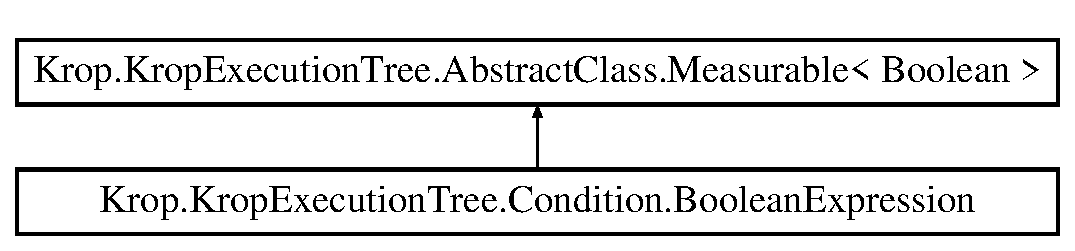
\includegraphics[height=2.000000cm]{class_krop_1_1_krop_execution_tree_1_1_condition_1_1_boolean_expression}
\end{center}
\end{figure}
\subsection*{Public Member Functions}
\begin{DoxyCompactItemize}
\item 
\mbox{\hyperlink{class_krop_1_1_krop_execution_tree_1_1_condition_1_1_boolean_expression_ab7d652f5fcf1d92ce165e553e1f0db2c}{Boolean\+Expression}} (Node \+\_\+node\+Boolean\+Expression, \mbox{\hyperlink{class_krop_1_1_krop_execution_tree_1_1_subprogram}{Subprogram}} \+\_\+parent\+Subprogram, bool \+\_\+is\+Not)
\item 
override bool \mbox{\hyperlink{class_krop_1_1_krop_execution_tree_1_1_condition_1_1_boolean_expression_a0d5dccaa10e9fa7933cf96edd1e670dd}{Evaluate}} ()
\begin{DoxyCompactList}\small\item\em Trigger the computation of the expression \end{DoxyCompactList}\end{DoxyCompactItemize}


\subsection{Detailed Description}
Holds a Boolean expression 



\subsection{Constructor \& Destructor Documentation}
\mbox{\Hypertarget{class_krop_1_1_krop_execution_tree_1_1_condition_1_1_boolean_expression_ab7d652f5fcf1d92ce165e553e1f0db2c}\label{class_krop_1_1_krop_execution_tree_1_1_condition_1_1_boolean_expression_ab7d652f5fcf1d92ce165e553e1f0db2c}} 
\index{Krop\+::\+Krop\+Execution\+Tree\+::\+Condition\+::\+Boolean\+Expression@{Krop\+::\+Krop\+Execution\+Tree\+::\+Condition\+::\+Boolean\+Expression}!Boolean\+Expression@{Boolean\+Expression}}
\index{Boolean\+Expression@{Boolean\+Expression}!Krop\+::\+Krop\+Execution\+Tree\+::\+Condition\+::\+Boolean\+Expression@{Krop\+::\+Krop\+Execution\+Tree\+::\+Condition\+::\+Boolean\+Expression}}
\subsubsection{\texorpdfstring{Boolean\+Expression()}{BooleanExpression()}}
{\footnotesize\ttfamily Krop.\+Krop\+Execution\+Tree.\+Condition.\+Boolean\+Expression.\+Boolean\+Expression (\begin{DoxyParamCaption}\item[{Node}]{\+\_\+node\+Boolean\+Expression,  }\item[{\mbox{\hyperlink{class_krop_1_1_krop_execution_tree_1_1_subprogram}{Subprogram}}}]{\+\_\+parent\+Subprogram,  }\item[{bool}]{\+\_\+is\+Not }\end{DoxyParamCaption})}



\subsection{Member Function Documentation}
\mbox{\Hypertarget{class_krop_1_1_krop_execution_tree_1_1_condition_1_1_boolean_expression_a0d5dccaa10e9fa7933cf96edd1e670dd}\label{class_krop_1_1_krop_execution_tree_1_1_condition_1_1_boolean_expression_a0d5dccaa10e9fa7933cf96edd1e670dd}} 
\index{Krop\+::\+Krop\+Execution\+Tree\+::\+Condition\+::\+Boolean\+Expression@{Krop\+::\+Krop\+Execution\+Tree\+::\+Condition\+::\+Boolean\+Expression}!Evaluate@{Evaluate}}
\index{Evaluate@{Evaluate}!Krop\+::\+Krop\+Execution\+Tree\+::\+Condition\+::\+Boolean\+Expression@{Krop\+::\+Krop\+Execution\+Tree\+::\+Condition\+::\+Boolean\+Expression}}
\subsubsection{\texorpdfstring{Evaluate()}{Evaluate()}}
{\footnotesize\ttfamily override bool Krop.\+Krop\+Execution\+Tree.\+Condition.\+Boolean\+Expression.\+Evaluate (\begin{DoxyParamCaption}{ }\end{DoxyParamCaption})\hspace{0.3cm}{\ttfamily [virtual]}}



Trigger the computation of the expression 

\begin{DoxyReturn}{Returns}
The result of the computation 
\end{DoxyReturn}


Implements \mbox{\hyperlink{class_krop_1_1_krop_execution_tree_1_1_abstract_class_1_1_measurable_afe91c739e2db11c8f316b07e8f55f7bb}{Krop.\+Krop\+Execution\+Tree.\+Abstract\+Class.\+Measurable$<$ Boolean $>$}}.



The documentation for this class was generated from the following file\+:\begin{DoxyCompactItemize}
\item 
C\+:/\+Users/\+Stuart.\+G\+U\+E\+I\+S\+S\+A\+Z/\+Documents/\+Git\+Hub/\+Krop/\+Code/\+Krop/\+Krop\+Execution\+Tree/\+Condition/\mbox{\hyperlink{_boolean_expression_8cs}{Boolean\+Expression.\+cs}}\end{DoxyCompactItemize}

\hypertarget{class_krop_1_1_krop_execution_tree_1_1_condition_1_1_boolean_function}{}\section{Krop.\+Krop\+Execution\+Tree.\+Condition.\+Boolean\+Function Class Reference}
\label{class_krop_1_1_krop_execution_tree_1_1_condition_1_1_boolean_function}\index{Krop.\+Krop\+Execution\+Tree.\+Condition.\+Boolean\+Function@{Krop.\+Krop\+Execution\+Tree.\+Condition.\+Boolean\+Function}}


Holds a Boolean variable  


Inheritance diagram for Krop.\+Krop\+Execution\+Tree.\+Condition.\+Boolean\+Function\+:\begin{figure}[H]
\begin{center}
\leavevmode
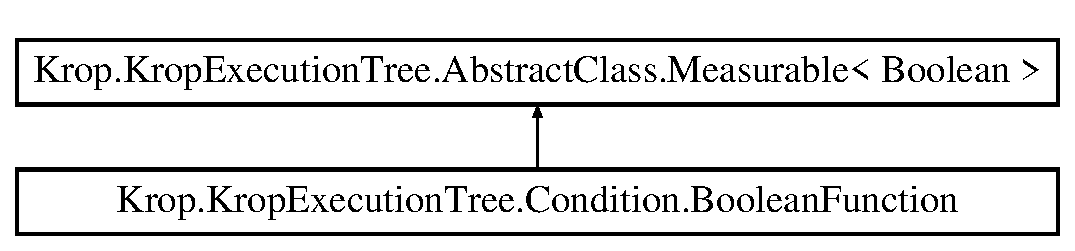
\includegraphics[height=2.000000cm]{class_krop_1_1_krop_execution_tree_1_1_condition_1_1_boolean_function}
\end{center}
\end{figure}
\subsection*{Public Member Functions}
\begin{DoxyCompactItemize}
\item 
\mbox{\hyperlink{class_krop_1_1_krop_execution_tree_1_1_condition_1_1_boolean_function_aaa2dc5cd14ba857edb9afaf22503d612}{Boolean\+Function}} (string \+\_\+name\+Function, Boolean \+\_\+is\+Not)
\item 
override bool \mbox{\hyperlink{class_krop_1_1_krop_execution_tree_1_1_condition_1_1_boolean_function_a1e274ef1079b4ab8136c45b5f48c747e}{Evaluate}} ()
\begin{DoxyCompactList}\small\item\em Trigger the computation of the expression \end{DoxyCompactList}\end{DoxyCompactItemize}


\subsection{Detailed Description}
Holds a Boolean variable 



\subsection{Constructor \& Destructor Documentation}
\mbox{\Hypertarget{class_krop_1_1_krop_execution_tree_1_1_condition_1_1_boolean_function_aaa2dc5cd14ba857edb9afaf22503d612}\label{class_krop_1_1_krop_execution_tree_1_1_condition_1_1_boolean_function_aaa2dc5cd14ba857edb9afaf22503d612}} 
\index{Krop\+::\+Krop\+Execution\+Tree\+::\+Condition\+::\+Boolean\+Function@{Krop\+::\+Krop\+Execution\+Tree\+::\+Condition\+::\+Boolean\+Function}!Boolean\+Function@{Boolean\+Function}}
\index{Boolean\+Function@{Boolean\+Function}!Krop\+::\+Krop\+Execution\+Tree\+::\+Condition\+::\+Boolean\+Function@{Krop\+::\+Krop\+Execution\+Tree\+::\+Condition\+::\+Boolean\+Function}}
\subsubsection{\texorpdfstring{Boolean\+Function()}{BooleanFunction()}}
{\footnotesize\ttfamily Krop.\+Krop\+Execution\+Tree.\+Condition.\+Boolean\+Function.\+Boolean\+Function (\begin{DoxyParamCaption}\item[{string}]{\+\_\+name\+Function,  }\item[{Boolean}]{\+\_\+is\+Not }\end{DoxyParamCaption})}



\subsection{Member Function Documentation}
\mbox{\Hypertarget{class_krop_1_1_krop_execution_tree_1_1_condition_1_1_boolean_function_a1e274ef1079b4ab8136c45b5f48c747e}\label{class_krop_1_1_krop_execution_tree_1_1_condition_1_1_boolean_function_a1e274ef1079b4ab8136c45b5f48c747e}} 
\index{Krop\+::\+Krop\+Execution\+Tree\+::\+Condition\+::\+Boolean\+Function@{Krop\+::\+Krop\+Execution\+Tree\+::\+Condition\+::\+Boolean\+Function}!Evaluate@{Evaluate}}
\index{Evaluate@{Evaluate}!Krop\+::\+Krop\+Execution\+Tree\+::\+Condition\+::\+Boolean\+Function@{Krop\+::\+Krop\+Execution\+Tree\+::\+Condition\+::\+Boolean\+Function}}
\subsubsection{\texorpdfstring{Evaluate()}{Evaluate()}}
{\footnotesize\ttfamily override bool Krop.\+Krop\+Execution\+Tree.\+Condition.\+Boolean\+Function.\+Evaluate (\begin{DoxyParamCaption}{ }\end{DoxyParamCaption})\hspace{0.3cm}{\ttfamily [virtual]}}



Trigger the computation of the expression 

\begin{DoxyReturn}{Returns}
The result of the computation 
\end{DoxyReturn}


Implements \mbox{\hyperlink{class_krop_1_1_krop_execution_tree_1_1_abstract_class_1_1_measurable_afe91c739e2db11c8f316b07e8f55f7bb}{Krop.\+Krop\+Execution\+Tree.\+Abstract\+Class.\+Measurable$<$ Boolean $>$}}.



The documentation for this class was generated from the following file\+:\begin{DoxyCompactItemize}
\item 
C\+:/\+Users/\+Stuart.\+G\+U\+E\+I\+S\+S\+A\+Z/\+Documents/\+Git\+Hub/\+Krop/\+Code/\+Krop/\+Krop\+Execution\+Tree/\+Condition/\mbox{\hyperlink{_boolean_function_8cs}{Boolean\+Function.\+cs}}\end{DoxyCompactItemize}

\hypertarget{class_krop_1_1_krop_execution_tree_1_1_condition_1_1_boolean_var}{}\section{Krop.\+Krop\+Execution\+Tree.\+Condition.\+Boolean\+Var Class Reference}
\label{class_krop_1_1_krop_execution_tree_1_1_condition_1_1_boolean_var}\index{Krop.\+Krop\+Execution\+Tree.\+Condition.\+Boolean\+Var@{Krop.\+Krop\+Execution\+Tree.\+Condition.\+Boolean\+Var}}


Holds a Boolean variable  


Inheritance diagram for Krop.\+Krop\+Execution\+Tree.\+Condition.\+Boolean\+Var\+:\begin{figure}[H]
\begin{center}
\leavevmode
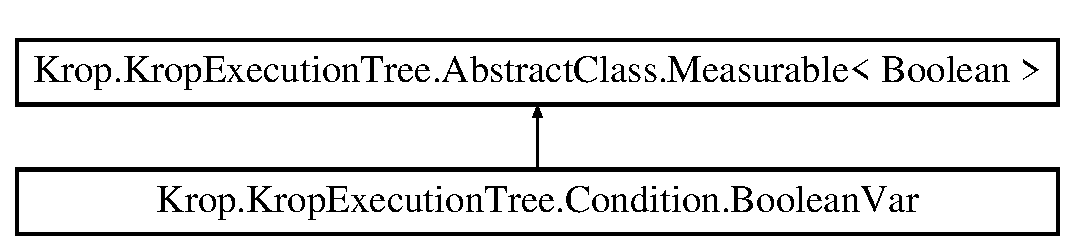
\includegraphics[height=2.000000cm]{class_krop_1_1_krop_execution_tree_1_1_condition_1_1_boolean_var}
\end{center}
\end{figure}
\subsection*{Public Member Functions}
\begin{DoxyCompactItemize}
\item 
\mbox{\hyperlink{class_krop_1_1_krop_execution_tree_1_1_condition_1_1_boolean_var_a33fb9a2ae3f57a06519bc3a300b602d6}{Boolean\+Var}} (Boolean \+\_\+value, Boolean \+\_\+is\+Not)
\item 
override bool \mbox{\hyperlink{class_krop_1_1_krop_execution_tree_1_1_condition_1_1_boolean_var_a293790e0485139dcf84fe9c35a5bac4a}{Evaluate}} ()
\begin{DoxyCompactList}\small\item\em Trigger the computation of the expression \end{DoxyCompactList}\end{DoxyCompactItemize}


\subsection{Detailed Description}
Holds a Boolean variable 



\subsection{Constructor \& Destructor Documentation}
\mbox{\Hypertarget{class_krop_1_1_krop_execution_tree_1_1_condition_1_1_boolean_var_a33fb9a2ae3f57a06519bc3a300b602d6}\label{class_krop_1_1_krop_execution_tree_1_1_condition_1_1_boolean_var_a33fb9a2ae3f57a06519bc3a300b602d6}} 
\index{Krop\+::\+Krop\+Execution\+Tree\+::\+Condition\+::\+Boolean\+Var@{Krop\+::\+Krop\+Execution\+Tree\+::\+Condition\+::\+Boolean\+Var}!Boolean\+Var@{Boolean\+Var}}
\index{Boolean\+Var@{Boolean\+Var}!Krop\+::\+Krop\+Execution\+Tree\+::\+Condition\+::\+Boolean\+Var@{Krop\+::\+Krop\+Execution\+Tree\+::\+Condition\+::\+Boolean\+Var}}
\subsubsection{\texorpdfstring{Boolean\+Var()}{BooleanVar()}}
{\footnotesize\ttfamily Krop.\+Krop\+Execution\+Tree.\+Condition.\+Boolean\+Var.\+Boolean\+Var (\begin{DoxyParamCaption}\item[{Boolean}]{\+\_\+value,  }\item[{Boolean}]{\+\_\+is\+Not }\end{DoxyParamCaption})}



\subsection{Member Function Documentation}
\mbox{\Hypertarget{class_krop_1_1_krop_execution_tree_1_1_condition_1_1_boolean_var_a293790e0485139dcf84fe9c35a5bac4a}\label{class_krop_1_1_krop_execution_tree_1_1_condition_1_1_boolean_var_a293790e0485139dcf84fe9c35a5bac4a}} 
\index{Krop\+::\+Krop\+Execution\+Tree\+::\+Condition\+::\+Boolean\+Var@{Krop\+::\+Krop\+Execution\+Tree\+::\+Condition\+::\+Boolean\+Var}!Evaluate@{Evaluate}}
\index{Evaluate@{Evaluate}!Krop\+::\+Krop\+Execution\+Tree\+::\+Condition\+::\+Boolean\+Var@{Krop\+::\+Krop\+Execution\+Tree\+::\+Condition\+::\+Boolean\+Var}}
\subsubsection{\texorpdfstring{Evaluate()}{Evaluate()}}
{\footnotesize\ttfamily override bool Krop.\+Krop\+Execution\+Tree.\+Condition.\+Boolean\+Var.\+Evaluate (\begin{DoxyParamCaption}{ }\end{DoxyParamCaption})\hspace{0.3cm}{\ttfamily [virtual]}}



Trigger the computation of the expression 

\begin{DoxyReturn}{Returns}
The result of the computation 
\end{DoxyReturn}


Implements \mbox{\hyperlink{class_krop_1_1_krop_execution_tree_1_1_abstract_class_1_1_measurable_afe91c739e2db11c8f316b07e8f55f7bb}{Krop.\+Krop\+Execution\+Tree.\+Abstract\+Class.\+Measurable$<$ Boolean $>$}}.



The documentation for this class was generated from the following file\+:\begin{DoxyCompactItemize}
\item 
C\+:/\+Users/\+Stuart.\+G\+U\+E\+I\+S\+S\+A\+Z/\+Documents/\+Git\+Hub/\+Krop/\+Code/\+Krop/\+Krop\+Execution\+Tree/\+Condition/\mbox{\hyperlink{_boolean_var_8cs}{Boolean\+Var.\+cs}}\end{DoxyCompactItemize}

\hypertarget{class_krop_1_1_krop_execution_tree_1_1_instruction_1_1_command}{}\section{Krop.\+Krop\+Execution\+Tree.\+Instruction.\+Command Class Reference}
\label{class_krop_1_1_krop_execution_tree_1_1_instruction_1_1_command}\index{Krop.\+Krop\+Execution\+Tree.\+Instruction.\+Command@{Krop.\+Krop\+Execution\+Tree.\+Instruction.\+Command}}


Holds a single known command  


Inheritance diagram for Krop.\+Krop\+Execution\+Tree.\+Instruction.\+Command\+:\begin{figure}[H]
\begin{center}
\leavevmode
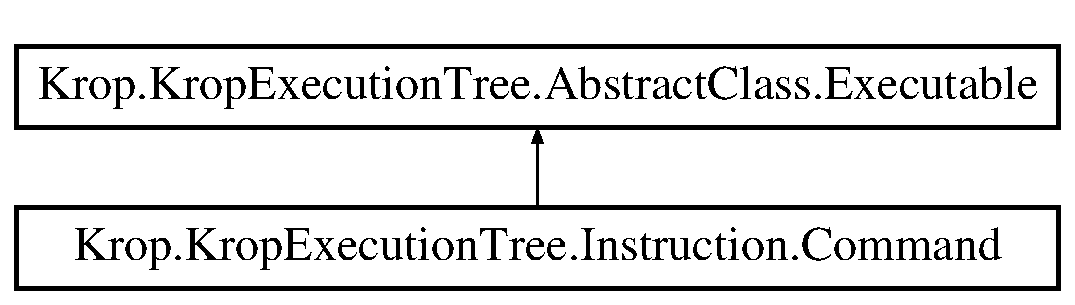
\includegraphics[height=2.000000cm]{class_krop_1_1_krop_execution_tree_1_1_instruction_1_1_command}
\end{center}
\end{figure}
\subsection*{Public Member Functions}
\begin{DoxyCompactItemize}
\item 
\mbox{\hyperlink{class_krop_1_1_krop_execution_tree_1_1_instruction_1_1_command_a2b946e88b50cff120ddd2a3946c77b70}{Command}} (Token \+\_\+token\+Instruction)
\item 
override bool \mbox{\hyperlink{class_krop_1_1_krop_execution_tree_1_1_instruction_1_1_command_ab0fc1d51e07e167cea0262e55e0de8af}{Execute}} ()
\end{DoxyCompactItemize}


\subsection{Detailed Description}
Holds a single known command 



\subsection{Constructor \& Destructor Documentation}
\mbox{\Hypertarget{class_krop_1_1_krop_execution_tree_1_1_instruction_1_1_command_a2b946e88b50cff120ddd2a3946c77b70}\label{class_krop_1_1_krop_execution_tree_1_1_instruction_1_1_command_a2b946e88b50cff120ddd2a3946c77b70}} 
\index{Krop\+::\+Krop\+Execution\+Tree\+::\+Instruction\+::\+Command@{Krop\+::\+Krop\+Execution\+Tree\+::\+Instruction\+::\+Command}!Command@{Command}}
\index{Command@{Command}!Krop\+::\+Krop\+Execution\+Tree\+::\+Instruction\+::\+Command@{Krop\+::\+Krop\+Execution\+Tree\+::\+Instruction\+::\+Command}}
\subsubsection{\texorpdfstring{Command()}{Command()}}
{\footnotesize\ttfamily Krop.\+Krop\+Execution\+Tree.\+Instruction.\+Command.\+Command (\begin{DoxyParamCaption}\item[{Token}]{\+\_\+token\+Instruction }\end{DoxyParamCaption})}



\subsection{Member Function Documentation}
\mbox{\Hypertarget{class_krop_1_1_krop_execution_tree_1_1_instruction_1_1_command_ab0fc1d51e07e167cea0262e55e0de8af}\label{class_krop_1_1_krop_execution_tree_1_1_instruction_1_1_command_ab0fc1d51e07e167cea0262e55e0de8af}} 
\index{Krop\+::\+Krop\+Execution\+Tree\+::\+Instruction\+::\+Command@{Krop\+::\+Krop\+Execution\+Tree\+::\+Instruction\+::\+Command}!Execute@{Execute}}
\index{Execute@{Execute}!Krop\+::\+Krop\+Execution\+Tree\+::\+Instruction\+::\+Command@{Krop\+::\+Krop\+Execution\+Tree\+::\+Instruction\+::\+Command}}
\subsubsection{\texorpdfstring{Execute()}{Execute()}}
{\footnotesize\ttfamily override bool Krop.\+Krop\+Execution\+Tree.\+Instruction.\+Command.\+Execute (\begin{DoxyParamCaption}{ }\end{DoxyParamCaption})\hspace{0.3cm}{\ttfamily [virtual]}}



Implements \mbox{\hyperlink{class_krop_1_1_krop_execution_tree_1_1_abstract_class_1_1_executable_ac32692ce44b5f938a90111ee27e7b684}{Krop.\+Krop\+Execution\+Tree.\+Abstract\+Class.\+Executable}}.



The documentation for this class was generated from the following file\+:\begin{DoxyCompactItemize}
\item 
C\+:/\+Users/\+Stuart.\+G\+U\+E\+I\+S\+S\+A\+Z/\+Documents/\+Git\+Hub/\+Krop/\+Code/\+Krop/\+Krop\+Execution\+Tree/\+Instruction/\mbox{\hyperlink{_command_8cs}{Command.\+cs}}\end{DoxyCompactItemize}

\hypertarget{class_krop_1_1_krohonde_1_1_content_pipe}{}\section{Krop.\+Krohonde.\+Content\+Pipe Class Reference}
\label{class_krop_1_1_krohonde_1_1_content_pipe}\index{Krop.\+Krohonde.\+Content\+Pipe@{Krop.\+Krohonde.\+Content\+Pipe}}
\subsection*{Static Public Member Functions}
\begin{DoxyCompactItemize}
\item 
static \mbox{\hyperlink{class_krop_1_1_krohonde_1_1_texture2_d}{Texture2D}} \mbox{\hyperlink{class_krop_1_1_krohonde_1_1_content_pipe_a4ff8f6d125632a87926b35e3bb8c8ada}{Load\+Texture}} (string path)
\end{DoxyCompactItemize}


\subsection{Member Function Documentation}
\mbox{\Hypertarget{class_krop_1_1_krohonde_1_1_content_pipe_a4ff8f6d125632a87926b35e3bb8c8ada}\label{class_krop_1_1_krohonde_1_1_content_pipe_a4ff8f6d125632a87926b35e3bb8c8ada}} 
\index{Krop\+::\+Krohonde\+::\+Content\+Pipe@{Krop\+::\+Krohonde\+::\+Content\+Pipe}!Load\+Texture@{Load\+Texture}}
\index{Load\+Texture@{Load\+Texture}!Krop\+::\+Krohonde\+::\+Content\+Pipe@{Krop\+::\+Krohonde\+::\+Content\+Pipe}}
\subsubsection{\texorpdfstring{Load\+Texture()}{LoadTexture()}}
{\footnotesize\ttfamily static \mbox{\hyperlink{class_krop_1_1_krohonde_1_1_texture2_d}{Texture2D}} Krop.\+Krohonde.\+Content\+Pipe.\+Load\+Texture (\begin{DoxyParamCaption}\item[{string}]{path }\end{DoxyParamCaption})\hspace{0.3cm}{\ttfamily [static]}}



The documentation for this class was generated from the following file\+:\begin{DoxyCompactItemize}
\item 
C\+:/\+Users/\+Stuart.\+G\+U\+E\+I\+S\+S\+A\+Z/\+Documents/\+Git\+Hub/\+Krop/\+Code/\+Krop/\+Krohonde/\mbox{\hyperlink{_content_pipe_8cs}{Content\+Pipe.\+cs}}\end{DoxyCompactItemize}

\hypertarget{class_krop_1_1_krop_execution_tree_1_1_abstract_class_1_1_executable}{}\section{Krop.\+Krop\+Execution\+Tree.\+Abstract\+Class.\+Executable Class Reference}
\label{class_krop_1_1_krop_execution_tree_1_1_abstract_class_1_1_executable}\index{Krop.\+Krop\+Execution\+Tree.\+Abstract\+Class.\+Executable@{Krop.\+Krop\+Execution\+Tree.\+Abstract\+Class.\+Executable}}


\mbox{\hyperlink{class_krop_1_1_krop_execution_tree_1_1_abstract_class_1_1_executable}{Executable}} objects are either a single command or a list thereof that can be executed Return true if successful  


Inheritance diagram for Krop.\+Krop\+Execution\+Tree.\+Abstract\+Class.\+Executable\+:\begin{figure}[H]
\begin{center}
\leavevmode
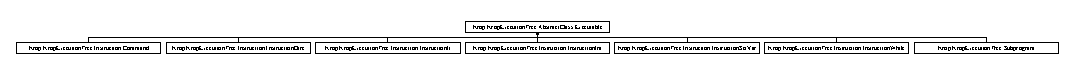
\includegraphics[height=0.496894cm]{class_krop_1_1_krop_execution_tree_1_1_abstract_class_1_1_executable}
\end{center}
\end{figure}
\subsection*{Public Member Functions}
\begin{DoxyCompactItemize}
\item 
abstract Boolean \mbox{\hyperlink{class_krop_1_1_krop_execution_tree_1_1_abstract_class_1_1_executable_ac32692ce44b5f938a90111ee27e7b684}{Execute}} ()
\item 
bool \mbox{\hyperlink{class_krop_1_1_krop_execution_tree_1_1_abstract_class_1_1_executable_a6a68e24e46c40a04ac71c7d71bbc2abd}{Can\+Execute}} ()
\begin{DoxyCompactList}\small\item\em Wait ending previous order, during pause or stop execution if clicking on Stop button \end{DoxyCompactList}\end{DoxyCompactItemize}


\subsection{Detailed Description}
\mbox{\hyperlink{class_krop_1_1_krop_execution_tree_1_1_abstract_class_1_1_executable}{Executable}} objects are either a single command or a list thereof that can be executed Return true if successful 



\subsection{Member Function Documentation}
\mbox{\Hypertarget{class_krop_1_1_krop_execution_tree_1_1_abstract_class_1_1_executable_a6a68e24e46c40a04ac71c7d71bbc2abd}\label{class_krop_1_1_krop_execution_tree_1_1_abstract_class_1_1_executable_a6a68e24e46c40a04ac71c7d71bbc2abd}} 
\index{Krop\+::\+Krop\+Execution\+Tree\+::\+Abstract\+Class\+::\+Executable@{Krop\+::\+Krop\+Execution\+Tree\+::\+Abstract\+Class\+::\+Executable}!Can\+Execute@{Can\+Execute}}
\index{Can\+Execute@{Can\+Execute}!Krop\+::\+Krop\+Execution\+Tree\+::\+Abstract\+Class\+::\+Executable@{Krop\+::\+Krop\+Execution\+Tree\+::\+Abstract\+Class\+::\+Executable}}
\subsubsection{\texorpdfstring{Can\+Execute()}{CanExecute()}}
{\footnotesize\ttfamily bool Krop.\+Krop\+Execution\+Tree.\+Abstract\+Class.\+Executable.\+Can\+Execute (\begin{DoxyParamCaption}{ }\end{DoxyParamCaption})}



Wait ending previous order, during pause or stop execution if clicking on Stop button 

\begin{DoxyReturn}{Returns}

\end{DoxyReturn}
\mbox{\Hypertarget{class_krop_1_1_krop_execution_tree_1_1_abstract_class_1_1_executable_ac32692ce44b5f938a90111ee27e7b684}\label{class_krop_1_1_krop_execution_tree_1_1_abstract_class_1_1_executable_ac32692ce44b5f938a90111ee27e7b684}} 
\index{Krop\+::\+Krop\+Execution\+Tree\+::\+Abstract\+Class\+::\+Executable@{Krop\+::\+Krop\+Execution\+Tree\+::\+Abstract\+Class\+::\+Executable}!Execute@{Execute}}
\index{Execute@{Execute}!Krop\+::\+Krop\+Execution\+Tree\+::\+Abstract\+Class\+::\+Executable@{Krop\+::\+Krop\+Execution\+Tree\+::\+Abstract\+Class\+::\+Executable}}
\subsubsection{\texorpdfstring{Execute()}{Execute()}}
{\footnotesize\ttfamily abstract Boolean Krop.\+Krop\+Execution\+Tree.\+Abstract\+Class.\+Executable.\+Execute (\begin{DoxyParamCaption}{ }\end{DoxyParamCaption})\hspace{0.3cm}{\ttfamily [pure virtual]}}



Implemented in \mbox{\hyperlink{class_krop_1_1_krop_execution_tree_1_1_subprogram_ae33466ddf0761f860c5817a4263efd29}{Krop.\+Krop\+Execution\+Tree.\+Subprogram}}, \mbox{\hyperlink{class_krop_1_1_krop_execution_tree_1_1_instruction_1_1_instruction_if_a69ee340a90824643f703e28e2ab665a1}{Krop.\+Krop\+Execution\+Tree.\+Instruction.\+Instruction\+If}}, \mbox{\hyperlink{class_krop_1_1_krop_execution_tree_1_1_instruction_1_1_instruction_dire_aef86c4e6b9ac3a4d17ed0c88db50a894}{Krop.\+Krop\+Execution\+Tree.\+Instruction.\+Instruction\+Dire}}, \mbox{\hyperlink{class_krop_1_1_krop_execution_tree_1_1_instruction_1_1_instruction_int_ac2e3bee4e5a115c09e03815df9f6ae0e}{Krop.\+Krop\+Execution\+Tree.\+Instruction.\+Instruction\+Int}}, \mbox{\hyperlink{class_krop_1_1_krop_execution_tree_1_1_instruction_1_1_instruction_set_var_a1c6739bcdc66cc9f50a8c9810958ed9f}{Krop.\+Krop\+Execution\+Tree.\+Instruction.\+Instruction\+Set\+Var}}, \mbox{\hyperlink{class_krop_1_1_krop_execution_tree_1_1_instruction_1_1_instruction_while_a98200d1758042e65604af4ad3cf95c9c}{Krop.\+Krop\+Execution\+Tree.\+Instruction.\+Instruction\+While}}, and \mbox{\hyperlink{class_krop_1_1_krop_execution_tree_1_1_instruction_1_1_command_ab0fc1d51e07e167cea0262e55e0de8af}{Krop.\+Krop\+Execution\+Tree.\+Instruction.\+Command}}.



The documentation for this class was generated from the following file\+:\begin{DoxyCompactItemize}
\item 
C\+:/\+Users/\+Stuart.\+G\+U\+E\+I\+S\+S\+A\+Z/\+Documents/\+Git\+Hub/\+Krop/\+Code/\+Krop/\+Krop\+Execution\+Tree/\+Abstract\+Class/\mbox{\hyperlink{_executable_8cs}{Executable.\+cs}}\end{DoxyCompactItemize}

\hypertarget{class_krop_1_1_control_window_1_1_form_control_window}{}\section{Krop.\+Control\+Window.\+Form\+Control\+Window Class Reference}
\label{class_krop_1_1_control_window_1_1_form_control_window}\index{Krop.\+Control\+Window.\+Form\+Control\+Window@{Krop.\+Control\+Window.\+Form\+Control\+Window}}
Inheritance diagram for Krop.\+Control\+Window.\+Form\+Control\+Window\+:\begin{figure}[H]
\begin{center}
\leavevmode
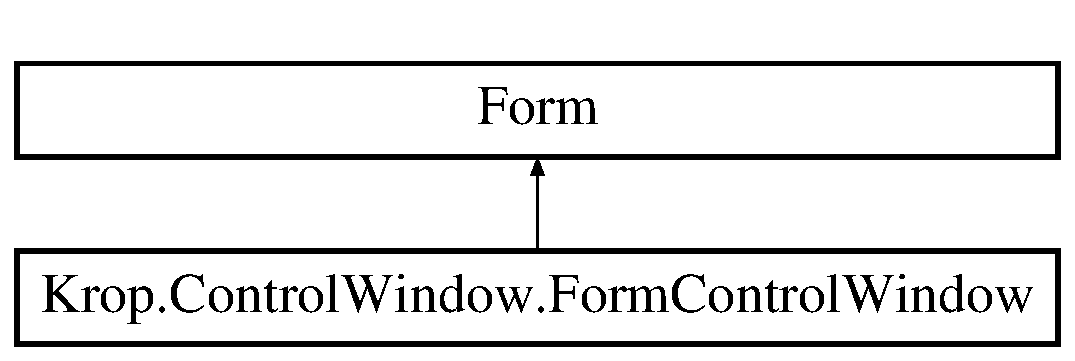
\includegraphics[height=2.000000cm]{class_krop_1_1_control_window_1_1_form_control_window}
\end{center}
\end{figure}
\subsection*{Public Member Functions}
\begin{DoxyCompactItemize}
\item 
\mbox{\hyperlink{class_krop_1_1_control_window_1_1_form_control_window_a094e44c9dbbe99ed8b83f63a1fc923b3}{Form\+Control\+Window}} ()
\begin{DoxyCompactList}\small\item\em Initialize Control Window \end{DoxyCompactList}\item 
void \mbox{\hyperlink{class_krop_1_1_control_window_1_1_form_control_window_a2b631b3483ebce4ba41da11c5a4b6cbd}{Initialize\+Krohonde\+Window}} ()
\begin{DoxyCompactList}\small\item\em Inialize \mbox{\hyperlink{namespace_krop_1_1_krohonde}{Krohonde}} Window \end{DoxyCompactList}\item 
void \mbox{\hyperlink{class_krop_1_1_control_window_1_1_form_control_window_ac4bdb9aee85bfb9c8f637e6919a49351}{Ending\+Program}} ()
\begin{DoxyCompactList}\small\item\em End executed program \end{DoxyCompactList}\item 
void \mbox{\hyperlink{class_krop_1_1_control_window_1_1_form_control_window_a27bd413aa79e780a7f8d9284cdd8f72d}{Get\+Tree}} (Node \+\_\+node)
\begin{DoxyCompactList}\small\item\em Display Grammatica tree in the terminal \end{DoxyCompactList}\end{DoxyCompactItemize}
\subsection*{Static Public Member Functions}
\begin{DoxyCompactItemize}
\item 
static void \mbox{\hyperlink{class_krop_1_1_control_window_1_1_form_control_window_ad4a2df546b92af668c27a51dd34ff742}{Terminal\+Write\+Line}} (string \+\_\+value)
\begin{DoxyCompactList}\small\item\em Write in txt\+Terminal \end{DoxyCompactList}\end{DoxyCompactItemize}
\subsection*{Static Public Attributes}
\begin{DoxyCompactItemize}
\item 
static Boolean \mbox{\hyperlink{class_krop_1_1_control_window_1_1_form_control_window_a7f70ff208833a41e5ee46e885106c760}{I\+S\+\_\+\+P\+A\+U\+S\+I\+NG}} = false
\item 
static Boolean \mbox{\hyperlink{class_krop_1_1_control_window_1_1_form_control_window_a869d7fc6bad7daa7c17b54451ea095a3}{I\+S\+\_\+\+S\+T\+O\+P\+P\+I\+NG}} = false
\item 
static Boolean \mbox{\hyperlink{class_krop_1_1_control_window_1_1_form_control_window_a304e98ecb96cc411a13eb2e8c24927e9}{I\+S\+\_\+\+R\+U\+N\+N\+I\+NG}} = false
\item 
static Boolean \mbox{\hyperlink{class_krop_1_1_control_window_1_1_form_control_window_a129f6c5eea061453561be894ece0342c}{P\+E\+N\+D\+I\+N\+G\+\_\+\+I\+N\+S\+T\+R\+U\+C\+T\+I\+ON}} = false
\item 
static Text\+Box \mbox{\hyperlink{class_krop_1_1_control_window_1_1_form_control_window_a107b67a284d28a7540f4f2adc40d6ec8}{T\+X\+T\+\_\+\+T\+E\+R\+M\+I\+N\+AL}}
\end{DoxyCompactItemize}
\subsection*{Protected Member Functions}
\begin{DoxyCompactItemize}
\item 
override void \mbox{\hyperlink{class_krop_1_1_control_window_1_1_form_control_window_ae6a4c484c02d89dc7707644f20123fe4}{Dispose}} (bool disposing)
\begin{DoxyCompactList}\small\item\em Clean up any resources being used. \end{DoxyCompactList}\end{DoxyCompactItemize}


\subsection{Constructor \& Destructor Documentation}
\mbox{\Hypertarget{class_krop_1_1_control_window_1_1_form_control_window_a094e44c9dbbe99ed8b83f63a1fc923b3}\label{class_krop_1_1_control_window_1_1_form_control_window_a094e44c9dbbe99ed8b83f63a1fc923b3}} 
\index{Krop\+::\+Control\+Window\+::\+Form\+Control\+Window@{Krop\+::\+Control\+Window\+::\+Form\+Control\+Window}!Form\+Control\+Window@{Form\+Control\+Window}}
\index{Form\+Control\+Window@{Form\+Control\+Window}!Krop\+::\+Control\+Window\+::\+Form\+Control\+Window@{Krop\+::\+Control\+Window\+::\+Form\+Control\+Window}}
\subsubsection{\texorpdfstring{Form\+Control\+Window()}{FormControlWindow()}}
{\footnotesize\ttfamily Krop.\+Control\+Window.\+Form\+Control\+Window.\+Form\+Control\+Window (\begin{DoxyParamCaption}{ }\end{DoxyParamCaption})}



Initialize Control Window 



\subsection{Member Function Documentation}
\mbox{\Hypertarget{class_krop_1_1_control_window_1_1_form_control_window_ae6a4c484c02d89dc7707644f20123fe4}\label{class_krop_1_1_control_window_1_1_form_control_window_ae6a4c484c02d89dc7707644f20123fe4}} 
\index{Krop\+::\+Control\+Window\+::\+Form\+Control\+Window@{Krop\+::\+Control\+Window\+::\+Form\+Control\+Window}!Dispose@{Dispose}}
\index{Dispose@{Dispose}!Krop\+::\+Control\+Window\+::\+Form\+Control\+Window@{Krop\+::\+Control\+Window\+::\+Form\+Control\+Window}}
\subsubsection{\texorpdfstring{Dispose()}{Dispose()}}
{\footnotesize\ttfamily override void Krop.\+Control\+Window.\+Form\+Control\+Window.\+Dispose (\begin{DoxyParamCaption}\item[{bool}]{disposing }\end{DoxyParamCaption})\hspace{0.3cm}{\ttfamily [protected]}}



Clean up any resources being used. 


\begin{DoxyParams}{Parameters}
{\em disposing} & true if managed resources should be disposed; otherwise, false.\\
\hline
\end{DoxyParams}
\mbox{\Hypertarget{class_krop_1_1_control_window_1_1_form_control_window_ac4bdb9aee85bfb9c8f637e6919a49351}\label{class_krop_1_1_control_window_1_1_form_control_window_ac4bdb9aee85bfb9c8f637e6919a49351}} 
\index{Krop\+::\+Control\+Window\+::\+Form\+Control\+Window@{Krop\+::\+Control\+Window\+::\+Form\+Control\+Window}!Ending\+Program@{Ending\+Program}}
\index{Ending\+Program@{Ending\+Program}!Krop\+::\+Control\+Window\+::\+Form\+Control\+Window@{Krop\+::\+Control\+Window\+::\+Form\+Control\+Window}}
\subsubsection{\texorpdfstring{Ending\+Program()}{EndingProgram()}}
{\footnotesize\ttfamily void Krop.\+Control\+Window.\+Form\+Control\+Window.\+Ending\+Program (\begin{DoxyParamCaption}{ }\end{DoxyParamCaption})}



End executed program 

\mbox{\Hypertarget{class_krop_1_1_control_window_1_1_form_control_window_a27bd413aa79e780a7f8d9284cdd8f72d}\label{class_krop_1_1_control_window_1_1_form_control_window_a27bd413aa79e780a7f8d9284cdd8f72d}} 
\index{Krop\+::\+Control\+Window\+::\+Form\+Control\+Window@{Krop\+::\+Control\+Window\+::\+Form\+Control\+Window}!Get\+Tree@{Get\+Tree}}
\index{Get\+Tree@{Get\+Tree}!Krop\+::\+Control\+Window\+::\+Form\+Control\+Window@{Krop\+::\+Control\+Window\+::\+Form\+Control\+Window}}
\subsubsection{\texorpdfstring{Get\+Tree()}{GetTree()}}
{\footnotesize\ttfamily void Krop.\+Control\+Window.\+Form\+Control\+Window.\+Get\+Tree (\begin{DoxyParamCaption}\item[{Node}]{\+\_\+node }\end{DoxyParamCaption})}



Display Grammatica tree in the terminal 


\begin{DoxyParams}{Parameters}
{\em node} & \\
\hline
\end{DoxyParams}
\mbox{\Hypertarget{class_krop_1_1_control_window_1_1_form_control_window_a2b631b3483ebce4ba41da11c5a4b6cbd}\label{class_krop_1_1_control_window_1_1_form_control_window_a2b631b3483ebce4ba41da11c5a4b6cbd}} 
\index{Krop\+::\+Control\+Window\+::\+Form\+Control\+Window@{Krop\+::\+Control\+Window\+::\+Form\+Control\+Window}!Initialize\+Krohonde\+Window@{Initialize\+Krohonde\+Window}}
\index{Initialize\+Krohonde\+Window@{Initialize\+Krohonde\+Window}!Krop\+::\+Control\+Window\+::\+Form\+Control\+Window@{Krop\+::\+Control\+Window\+::\+Form\+Control\+Window}}
\subsubsection{\texorpdfstring{Initialize\+Krohonde\+Window()}{InitializeKrohondeWindow()}}
{\footnotesize\ttfamily void Krop.\+Control\+Window.\+Form\+Control\+Window.\+Initialize\+Krohonde\+Window (\begin{DoxyParamCaption}{ }\end{DoxyParamCaption})}



Inialize \mbox{\hyperlink{namespace_krop_1_1_krohonde}{Krohonde}} Window 

\mbox{\Hypertarget{class_krop_1_1_control_window_1_1_form_control_window_ad4a2df546b92af668c27a51dd34ff742}\label{class_krop_1_1_control_window_1_1_form_control_window_ad4a2df546b92af668c27a51dd34ff742}} 
\index{Krop\+::\+Control\+Window\+::\+Form\+Control\+Window@{Krop\+::\+Control\+Window\+::\+Form\+Control\+Window}!Terminal\+Write\+Line@{Terminal\+Write\+Line}}
\index{Terminal\+Write\+Line@{Terminal\+Write\+Line}!Krop\+::\+Control\+Window\+::\+Form\+Control\+Window@{Krop\+::\+Control\+Window\+::\+Form\+Control\+Window}}
\subsubsection{\texorpdfstring{Terminal\+Write\+Line()}{TerminalWriteLine()}}
{\footnotesize\ttfamily static void Krop.\+Control\+Window.\+Form\+Control\+Window.\+Terminal\+Write\+Line (\begin{DoxyParamCaption}\item[{string}]{\+\_\+value }\end{DoxyParamCaption})\hspace{0.3cm}{\ttfamily [static]}}



Write in txt\+Terminal 


\begin{DoxyParams}{Parameters}
{\em \+\_\+value} & \\
\hline
\end{DoxyParams}


\subsection{Member Data Documentation}
\mbox{\Hypertarget{class_krop_1_1_control_window_1_1_form_control_window_a7f70ff208833a41e5ee46e885106c760}\label{class_krop_1_1_control_window_1_1_form_control_window_a7f70ff208833a41e5ee46e885106c760}} 
\index{Krop\+::\+Control\+Window\+::\+Form\+Control\+Window@{Krop\+::\+Control\+Window\+::\+Form\+Control\+Window}!I\+S\+\_\+\+P\+A\+U\+S\+I\+NG@{I\+S\+\_\+\+P\+A\+U\+S\+I\+NG}}
\index{I\+S\+\_\+\+P\+A\+U\+S\+I\+NG@{I\+S\+\_\+\+P\+A\+U\+S\+I\+NG}!Krop\+::\+Control\+Window\+::\+Form\+Control\+Window@{Krop\+::\+Control\+Window\+::\+Form\+Control\+Window}}
\subsubsection{\texorpdfstring{I\+S\+\_\+\+P\+A\+U\+S\+I\+NG}{IS\_PAUSING}}
{\footnotesize\ttfamily Boolean Krop.\+Control\+Window.\+Form\+Control\+Window.\+I\+S\+\_\+\+P\+A\+U\+S\+I\+NG = false\hspace{0.3cm}{\ttfamily [static]}}

\mbox{\Hypertarget{class_krop_1_1_control_window_1_1_form_control_window_a304e98ecb96cc411a13eb2e8c24927e9}\label{class_krop_1_1_control_window_1_1_form_control_window_a304e98ecb96cc411a13eb2e8c24927e9}} 
\index{Krop\+::\+Control\+Window\+::\+Form\+Control\+Window@{Krop\+::\+Control\+Window\+::\+Form\+Control\+Window}!I\+S\+\_\+\+R\+U\+N\+N\+I\+NG@{I\+S\+\_\+\+R\+U\+N\+N\+I\+NG}}
\index{I\+S\+\_\+\+R\+U\+N\+N\+I\+NG@{I\+S\+\_\+\+R\+U\+N\+N\+I\+NG}!Krop\+::\+Control\+Window\+::\+Form\+Control\+Window@{Krop\+::\+Control\+Window\+::\+Form\+Control\+Window}}
\subsubsection{\texorpdfstring{I\+S\+\_\+\+R\+U\+N\+N\+I\+NG}{IS\_RUNNING}}
{\footnotesize\ttfamily Boolean Krop.\+Control\+Window.\+Form\+Control\+Window.\+I\+S\+\_\+\+R\+U\+N\+N\+I\+NG = false\hspace{0.3cm}{\ttfamily [static]}}

\mbox{\Hypertarget{class_krop_1_1_control_window_1_1_form_control_window_a869d7fc6bad7daa7c17b54451ea095a3}\label{class_krop_1_1_control_window_1_1_form_control_window_a869d7fc6bad7daa7c17b54451ea095a3}} 
\index{Krop\+::\+Control\+Window\+::\+Form\+Control\+Window@{Krop\+::\+Control\+Window\+::\+Form\+Control\+Window}!I\+S\+\_\+\+S\+T\+O\+P\+P\+I\+NG@{I\+S\+\_\+\+S\+T\+O\+P\+P\+I\+NG}}
\index{I\+S\+\_\+\+S\+T\+O\+P\+P\+I\+NG@{I\+S\+\_\+\+S\+T\+O\+P\+P\+I\+NG}!Krop\+::\+Control\+Window\+::\+Form\+Control\+Window@{Krop\+::\+Control\+Window\+::\+Form\+Control\+Window}}
\subsubsection{\texorpdfstring{I\+S\+\_\+\+S\+T\+O\+P\+P\+I\+NG}{IS\_STOPPING}}
{\footnotesize\ttfamily Boolean Krop.\+Control\+Window.\+Form\+Control\+Window.\+I\+S\+\_\+\+S\+T\+O\+P\+P\+I\+NG = false\hspace{0.3cm}{\ttfamily [static]}}

\mbox{\Hypertarget{class_krop_1_1_control_window_1_1_form_control_window_a129f6c5eea061453561be894ece0342c}\label{class_krop_1_1_control_window_1_1_form_control_window_a129f6c5eea061453561be894ece0342c}} 
\index{Krop\+::\+Control\+Window\+::\+Form\+Control\+Window@{Krop\+::\+Control\+Window\+::\+Form\+Control\+Window}!P\+E\+N\+D\+I\+N\+G\+\_\+\+I\+N\+S\+T\+R\+U\+C\+T\+I\+ON@{P\+E\+N\+D\+I\+N\+G\+\_\+\+I\+N\+S\+T\+R\+U\+C\+T\+I\+ON}}
\index{P\+E\+N\+D\+I\+N\+G\+\_\+\+I\+N\+S\+T\+R\+U\+C\+T\+I\+ON@{P\+E\+N\+D\+I\+N\+G\+\_\+\+I\+N\+S\+T\+R\+U\+C\+T\+I\+ON}!Krop\+::\+Control\+Window\+::\+Form\+Control\+Window@{Krop\+::\+Control\+Window\+::\+Form\+Control\+Window}}
\subsubsection{\texorpdfstring{P\+E\+N\+D\+I\+N\+G\+\_\+\+I\+N\+S\+T\+R\+U\+C\+T\+I\+ON}{PENDING\_INSTRUCTION}}
{\footnotesize\ttfamily Boolean Krop.\+Control\+Window.\+Form\+Control\+Window.\+P\+E\+N\+D\+I\+N\+G\+\_\+\+I\+N\+S\+T\+R\+U\+C\+T\+I\+ON = false\hspace{0.3cm}{\ttfamily [static]}}

\mbox{\Hypertarget{class_krop_1_1_control_window_1_1_form_control_window_a107b67a284d28a7540f4f2adc40d6ec8}\label{class_krop_1_1_control_window_1_1_form_control_window_a107b67a284d28a7540f4f2adc40d6ec8}} 
\index{Krop\+::\+Control\+Window\+::\+Form\+Control\+Window@{Krop\+::\+Control\+Window\+::\+Form\+Control\+Window}!T\+X\+T\+\_\+\+T\+E\+R\+M\+I\+N\+AL@{T\+X\+T\+\_\+\+T\+E\+R\+M\+I\+N\+AL}}
\index{T\+X\+T\+\_\+\+T\+E\+R\+M\+I\+N\+AL@{T\+X\+T\+\_\+\+T\+E\+R\+M\+I\+N\+AL}!Krop\+::\+Control\+Window\+::\+Form\+Control\+Window@{Krop\+::\+Control\+Window\+::\+Form\+Control\+Window}}
\subsubsection{\texorpdfstring{T\+X\+T\+\_\+\+T\+E\+R\+M\+I\+N\+AL}{TXT\_TERMINAL}}
{\footnotesize\ttfamily Text\+Box Krop.\+Control\+Window.\+Form\+Control\+Window.\+T\+X\+T\+\_\+\+T\+E\+R\+M\+I\+N\+AL\hspace{0.3cm}{\ttfamily [static]}}



The documentation for this class was generated from the following files\+:\begin{DoxyCompactItemize}
\item 
C\+:/\+Users/\+Stuart.\+G\+U\+E\+I\+S\+S\+A\+Z/\+Documents/\+Git\+Hub/\+Krop/\+Code/\+Krop/\+Control\+Window/\mbox{\hyperlink{_form_control_window_8cs}{Form\+Control\+Window.\+cs}}\item 
C\+:/\+Users/\+Stuart.\+G\+U\+E\+I\+S\+S\+A\+Z/\+Documents/\+Git\+Hub/\+Krop/\+Code/\+Krop/\+Control\+Window/\mbox{\hyperlink{_form_control_window_8_designer_8cs}{Form\+Control\+Window.\+Designer.\+cs}}\end{DoxyCompactItemize}

\hypertarget{class_krop_1_1_krohonde_1_1_game}{}\section{Krop.\+Krohonde.\+Game Class Reference}
\label{class_krop_1_1_krohonde_1_1_game}\index{Krop.\+Krohonde.\+Game@{Krop.\+Krohonde.\+Game}}


Primary class of the project  


Inheritance diagram for Krop.\+Krohonde.\+Game\+:\begin{figure}[H]
\begin{center}
\leavevmode
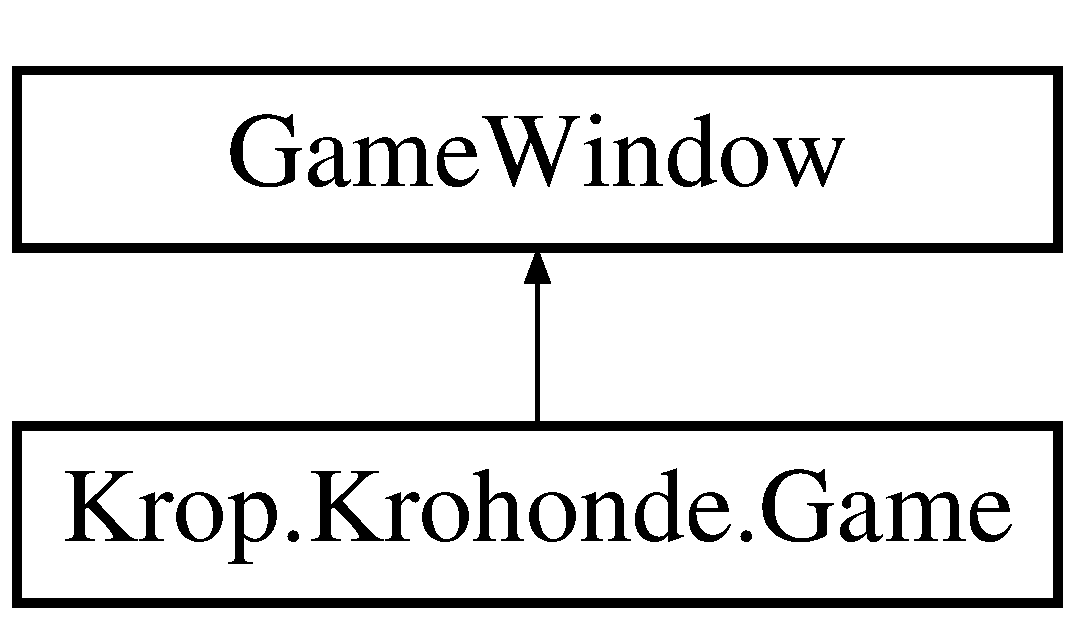
\includegraphics[height=2.000000cm]{class_krop_1_1_krohonde_1_1_game}
\end{center}
\end{figure}
\subsection*{Public Member Functions}
\begin{DoxyCompactItemize}
\item 
\mbox{\hyperlink{class_krop_1_1_krohonde_1_1_game_a99b4f31e791c00af369068b6a17482de}{Game}} (int width, int height)
\begin{DoxyCompactList}\small\item\em Create the game window \end{DoxyCompactList}\end{DoxyCompactItemize}
\subsection*{Static Public Member Functions}
\begin{DoxyCompactItemize}
\item 
static bool \mbox{\hyperlink{class_krop_1_1_krohonde_1_1_game_a1478a79991c3ede806daa5a2e6bb1f69}{Place\+Is\+Free}} (int \+\_\+posX, int \+\_\+posY)
\begin{DoxyCompactList}\small\item\em Check if the grid square is of type grass \end{DoxyCompactList}\item 
static bool \mbox{\hyperlink{class_krop_1_1_krohonde_1_1_game_a4cc704bda7106616a4d467743bf703d6}{On\+Pheromone}} ()
\begin{DoxyCompactList}\small\item\em Check if the ant is on a pheromone \end{DoxyCompactList}\item 
static void \mbox{\hyperlink{class_krop_1_1_krohonde_1_1_game_a4d1fe0a45ef3e7ef8600a3ccef1289b0}{Drop\+Pheromone}} ()
\begin{DoxyCompactList}\small\item\em Drop a pheromone below the ant \end{DoxyCompactList}\item 
static void \mbox{\hyperlink{class_krop_1_1_krohonde_1_1_game_a17afa697841f604772d61aaf2b8719f8}{Take\+Pheromone}} ()
\begin{DoxyCompactList}\small\item\em Take a pheromone below the ant \end{DoxyCompactList}\item 
static bool \mbox{\hyperlink{class_krop_1_1_krohonde_1_1_game_a4eef675c83400a1028687124abc72406}{Obstacle\+In\+Front}} ()
\begin{DoxyCompactList}\small\item\em Check if there is an obstacle in front of the ant \end{DoxyCompactList}\item 
static bool \mbox{\hyperlink{class_krop_1_1_krohonde_1_1_game_a7a4f81955b1da1871586ee8f311cc20e}{Obstacle\+On\+Right}} ()
\begin{DoxyCompactList}\small\item\em Check if there is an obstacle on the right of the ant \end{DoxyCompactList}\item 
static bool \mbox{\hyperlink{class_krop_1_1_krohonde_1_1_game_a6bca313b39a9effdc456b6a31f5af50f}{Obstacle\+On\+Left}} ()
\begin{DoxyCompactList}\small\item\em Check if there is an obstacle on the left of the ant \end{DoxyCompactList}\item 
static void \mbox{\hyperlink{class_krop_1_1_krohonde_1_1_game_ac51d3346621871ac6d5d7faff715a067}{Change\+Garden}} (string \+\_\+path)
\begin{DoxyCompactList}\small\item\em Load a garden \end{DoxyCompactList}\item 
static void \mbox{\hyperlink{class_krop_1_1_krohonde_1_1_game_ad89cd94c1649b695992d56fc9da54f35}{Change\+Garden}} (int \+\_\+x, int \+\_\+y)
\begin{DoxyCompactList}\small\item\em Load default garden \end{DoxyCompactList}\end{DoxyCompactItemize}
\subsection*{Static Public Attributes}
\begin{DoxyCompactItemize}
\item 
static bool \mbox{\hyperlink{class_krop_1_1_krohonde_1_1_game_a6a3e7db26ac0b9f80507bf6ea36d4fd2}{E\+X\+I\+T\+\_\+\+K\+R\+O\+H\+O\+N\+DE}} = false
\item 
static int \mbox{\hyperlink{class_krop_1_1_krohonde_1_1_game_a3cff1b81bcc3759e697aa76cee2d758e}{W\+I\+D\+T\+H\+W\+I\+N\+D\+OW}} = 960
\item 
static int \mbox{\hyperlink{class_krop_1_1_krohonde_1_1_game_ad75f5df73247858cd812bdeebb40d39e}{H\+E\+I\+G\+H\+T\+W\+I\+N\+D\+OW}} = 720
\item 
static int \mbox{\hyperlink{class_krop_1_1_krohonde_1_1_game_ae73d97c0f81728f4ff142d36ab9dde4d}{G\+R\+I\+D\+S\+I\+ZE}} = 24
\item 
static int \mbox{\hyperlink{class_krop_1_1_krohonde_1_1_game_a248438b8c8aa03b448ccf9203b0754e7}{H\+E\+I\+G\+H\+T\+G\+A\+R\+D\+EN}} = 30
\item 
static int \mbox{\hyperlink{class_krop_1_1_krohonde_1_1_game_a2e5966eba694146acb742074bd5d9ae3}{W\+I\+D\+T\+H\+G\+A\+R\+D\+EN}} = 40
\item 
static int \mbox{\hyperlink{class_krop_1_1_krohonde_1_1_game_a1351c196ec69b91703900e09a713f49a}{T\+I\+L\+E\+S\+I\+ZE}} = 32
\item 
static \mbox{\hyperlink{class_krop_1_1_krohonde_1_1_texture2_d}{Texture2D}} \mbox{\hyperlink{class_krop_1_1_krohonde_1_1_game_a58093d75ef6e73acbff1eb82c77cd9b9}{T\+I\+L\+E\+S\+ET}}
\item 
static \mbox{\hyperlink{class_krop_1_1_krohonde_1_1_ant}{Ant}} \mbox{\hyperlink{class_krop_1_1_krohonde_1_1_game_a985a69e1fe6b1e94b969ed3cffcc0ca4}{A\+NT}} = new \mbox{\hyperlink{class_krop_1_1_krohonde_1_1_ant}{Ant}}()
\end{DoxyCompactItemize}
\subsection*{Protected Member Functions}
\begin{DoxyCompactItemize}
\item 
override void \mbox{\hyperlink{class_krop_1_1_krohonde_1_1_game_a1d0295e8614a48b8a81552b209c5ed4a}{On\+Load}} (Event\+Args e)
\begin{DoxyCompactList}\small\item\em Start when the program loads \end{DoxyCompactList}\item 
override void \mbox{\hyperlink{class_krop_1_1_krohonde_1_1_game_ae417ed79f31ff0280ca92ec3202990e3}{On\+Closing}} (Cancel\+Event\+Args e)
\begin{DoxyCompactList}\small\item\em Close \mbox{\hyperlink{namespace_krop}{Krop}} \end{DoxyCompactList}\item 
override void \mbox{\hyperlink{class_krop_1_1_krohonde_1_1_game_ad88326ce1906f9e45caa3005781a70a2}{On\+Update\+Frame}} (Frame\+Event\+Args e)
\begin{DoxyCompactList}\small\item\em Start on each update frame This function starts all the calculation functions of the differents garden elements like the new position, the sprite \end{DoxyCompactList}\item 
override void \mbox{\hyperlink{class_krop_1_1_krohonde_1_1_game_ab12bfce981cec214fe7f8e35abd342eb}{On\+Render\+Frame}} (Frame\+Event\+Args e)
\begin{DoxyCompactList}\small\item\em Manage the elements display on the window \end{DoxyCompactList}\end{DoxyCompactItemize}


\subsection{Detailed Description}
Primary class of the project 



\subsection{Constructor \& Destructor Documentation}
\mbox{\Hypertarget{class_krop_1_1_krohonde_1_1_game_a99b4f31e791c00af369068b6a17482de}\label{class_krop_1_1_krohonde_1_1_game_a99b4f31e791c00af369068b6a17482de}} 
\index{Krop\+::\+Krohonde\+::\+Game@{Krop\+::\+Krohonde\+::\+Game}!Game@{Game}}
\index{Game@{Game}!Krop\+::\+Krohonde\+::\+Game@{Krop\+::\+Krohonde\+::\+Game}}
\subsubsection{\texorpdfstring{Game()}{Game()}}
{\footnotesize\ttfamily Krop.\+Krohonde.\+Game.\+Game (\begin{DoxyParamCaption}\item[{int}]{width,  }\item[{int}]{height }\end{DoxyParamCaption})}



Create the game window 


\begin{DoxyParams}{Parameters}
{\em width} & Number of grid columns\\
\hline
{\em height} & Number of grid rows\\
\hline
\end{DoxyParams}


\subsection{Member Function Documentation}
\mbox{\Hypertarget{class_krop_1_1_krohonde_1_1_game_ac51d3346621871ac6d5d7faff715a067}\label{class_krop_1_1_krohonde_1_1_game_ac51d3346621871ac6d5d7faff715a067}} 
\index{Krop\+::\+Krohonde\+::\+Game@{Krop\+::\+Krohonde\+::\+Game}!Change\+Garden@{Change\+Garden}}
\index{Change\+Garden@{Change\+Garden}!Krop\+::\+Krohonde\+::\+Game@{Krop\+::\+Krohonde\+::\+Game}}
\subsubsection{\texorpdfstring{Change\+Garden()}{ChangeGarden()}\hspace{0.1cm}{\footnotesize\ttfamily [1/2]}}
{\footnotesize\ttfamily static void Krop.\+Krohonde.\+Game.\+Change\+Garden (\begin{DoxyParamCaption}\item[{string}]{\+\_\+path }\end{DoxyParamCaption})\hspace{0.3cm}{\ttfamily [static]}}



Load a garden 


\begin{DoxyParams}{Parameters}
{\em \+\_\+path} & Name of the file containing garden \\
\hline
\end{DoxyParams}
\mbox{\Hypertarget{class_krop_1_1_krohonde_1_1_game_ad89cd94c1649b695992d56fc9da54f35}\label{class_krop_1_1_krohonde_1_1_game_ad89cd94c1649b695992d56fc9da54f35}} 
\index{Krop\+::\+Krohonde\+::\+Game@{Krop\+::\+Krohonde\+::\+Game}!Change\+Garden@{Change\+Garden}}
\index{Change\+Garden@{Change\+Garden}!Krop\+::\+Krohonde\+::\+Game@{Krop\+::\+Krohonde\+::\+Game}}
\subsubsection{\texorpdfstring{Change\+Garden()}{ChangeGarden()}\hspace{0.1cm}{\footnotesize\ttfamily [2/2]}}
{\footnotesize\ttfamily static void Krop.\+Krohonde.\+Game.\+Change\+Garden (\begin{DoxyParamCaption}\item[{int}]{\+\_\+x,  }\item[{int}]{\+\_\+y }\end{DoxyParamCaption})\hspace{0.3cm}{\ttfamily [static]}}



Load default garden 


\begin{DoxyParams}{Parameters}
{\em \+\_\+x} & Width of the garden\\
\hline
{\em \+\_\+y} & Height of the garden\\
\hline
\end{DoxyParams}
\mbox{\Hypertarget{class_krop_1_1_krohonde_1_1_game_a4d1fe0a45ef3e7ef8600a3ccef1289b0}\label{class_krop_1_1_krohonde_1_1_game_a4d1fe0a45ef3e7ef8600a3ccef1289b0}} 
\index{Krop\+::\+Krohonde\+::\+Game@{Krop\+::\+Krohonde\+::\+Game}!Drop\+Pheromone@{Drop\+Pheromone}}
\index{Drop\+Pheromone@{Drop\+Pheromone}!Krop\+::\+Krohonde\+::\+Game@{Krop\+::\+Krohonde\+::\+Game}}
\subsubsection{\texorpdfstring{Drop\+Pheromone()}{DropPheromone()}}
{\footnotesize\ttfamily static void Krop.\+Krohonde.\+Game.\+Drop\+Pheromone (\begin{DoxyParamCaption}{ }\end{DoxyParamCaption})\hspace{0.3cm}{\ttfamily [static]}}



Drop a pheromone below the ant 

\mbox{\Hypertarget{class_krop_1_1_krohonde_1_1_game_a4eef675c83400a1028687124abc72406}\label{class_krop_1_1_krohonde_1_1_game_a4eef675c83400a1028687124abc72406}} 
\index{Krop\+::\+Krohonde\+::\+Game@{Krop\+::\+Krohonde\+::\+Game}!Obstacle\+In\+Front@{Obstacle\+In\+Front}}
\index{Obstacle\+In\+Front@{Obstacle\+In\+Front}!Krop\+::\+Krohonde\+::\+Game@{Krop\+::\+Krohonde\+::\+Game}}
\subsubsection{\texorpdfstring{Obstacle\+In\+Front()}{ObstacleInFront()}}
{\footnotesize\ttfamily static bool Krop.\+Krohonde.\+Game.\+Obstacle\+In\+Front (\begin{DoxyParamCaption}{ }\end{DoxyParamCaption})\hspace{0.3cm}{\ttfamily [static]}}



Check if there is an obstacle in front of the ant 

\begin{DoxyReturn}{Returns}
Is\+Solid of the block
\end{DoxyReturn}
\mbox{\Hypertarget{class_krop_1_1_krohonde_1_1_game_a6bca313b39a9effdc456b6a31f5af50f}\label{class_krop_1_1_krohonde_1_1_game_a6bca313b39a9effdc456b6a31f5af50f}} 
\index{Krop\+::\+Krohonde\+::\+Game@{Krop\+::\+Krohonde\+::\+Game}!Obstacle\+On\+Left@{Obstacle\+On\+Left}}
\index{Obstacle\+On\+Left@{Obstacle\+On\+Left}!Krop\+::\+Krohonde\+::\+Game@{Krop\+::\+Krohonde\+::\+Game}}
\subsubsection{\texorpdfstring{Obstacle\+On\+Left()}{ObstacleOnLeft()}}
{\footnotesize\ttfamily static bool Krop.\+Krohonde.\+Game.\+Obstacle\+On\+Left (\begin{DoxyParamCaption}{ }\end{DoxyParamCaption})\hspace{0.3cm}{\ttfamily [static]}}



Check if there is an obstacle on the left of the ant 

\begin{DoxyReturn}{Returns}
Is\+Solid of the block
\end{DoxyReturn}
\mbox{\Hypertarget{class_krop_1_1_krohonde_1_1_game_a7a4f81955b1da1871586ee8f311cc20e}\label{class_krop_1_1_krohonde_1_1_game_a7a4f81955b1da1871586ee8f311cc20e}} 
\index{Krop\+::\+Krohonde\+::\+Game@{Krop\+::\+Krohonde\+::\+Game}!Obstacle\+On\+Right@{Obstacle\+On\+Right}}
\index{Obstacle\+On\+Right@{Obstacle\+On\+Right}!Krop\+::\+Krohonde\+::\+Game@{Krop\+::\+Krohonde\+::\+Game}}
\subsubsection{\texorpdfstring{Obstacle\+On\+Right()}{ObstacleOnRight()}}
{\footnotesize\ttfamily static bool Krop.\+Krohonde.\+Game.\+Obstacle\+On\+Right (\begin{DoxyParamCaption}{ }\end{DoxyParamCaption})\hspace{0.3cm}{\ttfamily [static]}}



Check if there is an obstacle on the right of the ant 

\begin{DoxyReturn}{Returns}
Is\+Solid of the block
\end{DoxyReturn}
\mbox{\Hypertarget{class_krop_1_1_krohonde_1_1_game_ae417ed79f31ff0280ca92ec3202990e3}\label{class_krop_1_1_krohonde_1_1_game_ae417ed79f31ff0280ca92ec3202990e3}} 
\index{Krop\+::\+Krohonde\+::\+Game@{Krop\+::\+Krohonde\+::\+Game}!On\+Closing@{On\+Closing}}
\index{On\+Closing@{On\+Closing}!Krop\+::\+Krohonde\+::\+Game@{Krop\+::\+Krohonde\+::\+Game}}
\subsubsection{\texorpdfstring{On\+Closing()}{OnClosing()}}
{\footnotesize\ttfamily override void Krop.\+Krohonde.\+Game.\+On\+Closing (\begin{DoxyParamCaption}\item[{Cancel\+Event\+Args}]{e }\end{DoxyParamCaption})\hspace{0.3cm}{\ttfamily [protected]}}



Close \mbox{\hyperlink{namespace_krop}{Krop}} 


\begin{DoxyParams}{Parameters}
{\em e} & \\
\hline
\end{DoxyParams}
\mbox{\Hypertarget{class_krop_1_1_krohonde_1_1_game_a1d0295e8614a48b8a81552b209c5ed4a}\label{class_krop_1_1_krohonde_1_1_game_a1d0295e8614a48b8a81552b209c5ed4a}} 
\index{Krop\+::\+Krohonde\+::\+Game@{Krop\+::\+Krohonde\+::\+Game}!On\+Load@{On\+Load}}
\index{On\+Load@{On\+Load}!Krop\+::\+Krohonde\+::\+Game@{Krop\+::\+Krohonde\+::\+Game}}
\subsubsection{\texorpdfstring{On\+Load()}{OnLoad()}}
{\footnotesize\ttfamily override void Krop.\+Krohonde.\+Game.\+On\+Load (\begin{DoxyParamCaption}\item[{Event\+Args}]{e }\end{DoxyParamCaption})\hspace{0.3cm}{\ttfamily [protected]}}



Start when the program loads 


\begin{DoxyParams}{Parameters}
{\em e} & \\
\hline
\end{DoxyParams}
\mbox{\Hypertarget{class_krop_1_1_krohonde_1_1_game_a4cc704bda7106616a4d467743bf703d6}\label{class_krop_1_1_krohonde_1_1_game_a4cc704bda7106616a4d467743bf703d6}} 
\index{Krop\+::\+Krohonde\+::\+Game@{Krop\+::\+Krohonde\+::\+Game}!On\+Pheromone@{On\+Pheromone}}
\index{On\+Pheromone@{On\+Pheromone}!Krop\+::\+Krohonde\+::\+Game@{Krop\+::\+Krohonde\+::\+Game}}
\subsubsection{\texorpdfstring{On\+Pheromone()}{OnPheromone()}}
{\footnotesize\ttfamily static bool Krop.\+Krohonde.\+Game.\+On\+Pheromone (\begin{DoxyParamCaption}{ }\end{DoxyParamCaption})\hspace{0.3cm}{\ttfamily [static]}}



Check if the ant is on a pheromone 

\begin{DoxyReturn}{Returns}
Is\+Pheromone of the block
\end{DoxyReturn}
\mbox{\Hypertarget{class_krop_1_1_krohonde_1_1_game_ab12bfce981cec214fe7f8e35abd342eb}\label{class_krop_1_1_krohonde_1_1_game_ab12bfce981cec214fe7f8e35abd342eb}} 
\index{Krop\+::\+Krohonde\+::\+Game@{Krop\+::\+Krohonde\+::\+Game}!On\+Render\+Frame@{On\+Render\+Frame}}
\index{On\+Render\+Frame@{On\+Render\+Frame}!Krop\+::\+Krohonde\+::\+Game@{Krop\+::\+Krohonde\+::\+Game}}
\subsubsection{\texorpdfstring{On\+Render\+Frame()}{OnRenderFrame()}}
{\footnotesize\ttfamily override void Krop.\+Krohonde.\+Game.\+On\+Render\+Frame (\begin{DoxyParamCaption}\item[{Frame\+Event\+Args}]{e }\end{DoxyParamCaption})\hspace{0.3cm}{\ttfamily [protected]}}



Manage the elements display on the window 


\begin{DoxyParams}{Parameters}
{\em e} & \\
\hline
\end{DoxyParams}
\mbox{\Hypertarget{class_krop_1_1_krohonde_1_1_game_ad88326ce1906f9e45caa3005781a70a2}\label{class_krop_1_1_krohonde_1_1_game_ad88326ce1906f9e45caa3005781a70a2}} 
\index{Krop\+::\+Krohonde\+::\+Game@{Krop\+::\+Krohonde\+::\+Game}!On\+Update\+Frame@{On\+Update\+Frame}}
\index{On\+Update\+Frame@{On\+Update\+Frame}!Krop\+::\+Krohonde\+::\+Game@{Krop\+::\+Krohonde\+::\+Game}}
\subsubsection{\texorpdfstring{On\+Update\+Frame()}{OnUpdateFrame()}}
{\footnotesize\ttfamily override void Krop.\+Krohonde.\+Game.\+On\+Update\+Frame (\begin{DoxyParamCaption}\item[{Frame\+Event\+Args}]{e }\end{DoxyParamCaption})\hspace{0.3cm}{\ttfamily [protected]}}



Start on each update frame This function starts all the calculation functions of the differents garden elements like the new position, the sprite 


\begin{DoxyParams}{Parameters}
{\em e} & \\
\hline
\end{DoxyParams}
\mbox{\Hypertarget{class_krop_1_1_krohonde_1_1_game_a1478a79991c3ede806daa5a2e6bb1f69}\label{class_krop_1_1_krohonde_1_1_game_a1478a79991c3ede806daa5a2e6bb1f69}} 
\index{Krop\+::\+Krohonde\+::\+Game@{Krop\+::\+Krohonde\+::\+Game}!Place\+Is\+Free@{Place\+Is\+Free}}
\index{Place\+Is\+Free@{Place\+Is\+Free}!Krop\+::\+Krohonde\+::\+Game@{Krop\+::\+Krohonde\+::\+Game}}
\subsubsection{\texorpdfstring{Place\+Is\+Free()}{PlaceIsFree()}}
{\footnotesize\ttfamily static bool Krop.\+Krohonde.\+Game.\+Place\+Is\+Free (\begin{DoxyParamCaption}\item[{int}]{\+\_\+posX,  }\item[{int}]{\+\_\+posY }\end{DoxyParamCaption})\hspace{0.3cm}{\ttfamily [static]}}



Check if the grid square is of type grass 


\begin{DoxyParams}{Parameters}
{\em \+\_\+posX} & \\
\hline
{\em \+\_\+posY} & \\
\hline
\end{DoxyParams}
\begin{DoxyReturn}{Returns}
!\+Is\+Solid of the block
\end{DoxyReturn}
\mbox{\Hypertarget{class_krop_1_1_krohonde_1_1_game_a17afa697841f604772d61aaf2b8719f8}\label{class_krop_1_1_krohonde_1_1_game_a17afa697841f604772d61aaf2b8719f8}} 
\index{Krop\+::\+Krohonde\+::\+Game@{Krop\+::\+Krohonde\+::\+Game}!Take\+Pheromone@{Take\+Pheromone}}
\index{Take\+Pheromone@{Take\+Pheromone}!Krop\+::\+Krohonde\+::\+Game@{Krop\+::\+Krohonde\+::\+Game}}
\subsubsection{\texorpdfstring{Take\+Pheromone()}{TakePheromone()}}
{\footnotesize\ttfamily static void Krop.\+Krohonde.\+Game.\+Take\+Pheromone (\begin{DoxyParamCaption}{ }\end{DoxyParamCaption})\hspace{0.3cm}{\ttfamily [static]}}



Take a pheromone below the ant 



\subsection{Member Data Documentation}
\mbox{\Hypertarget{class_krop_1_1_krohonde_1_1_game_a985a69e1fe6b1e94b969ed3cffcc0ca4}\label{class_krop_1_1_krohonde_1_1_game_a985a69e1fe6b1e94b969ed3cffcc0ca4}} 
\index{Krop\+::\+Krohonde\+::\+Game@{Krop\+::\+Krohonde\+::\+Game}!A\+NT@{A\+NT}}
\index{A\+NT@{A\+NT}!Krop\+::\+Krohonde\+::\+Game@{Krop\+::\+Krohonde\+::\+Game}}
\subsubsection{\texorpdfstring{A\+NT}{ANT}}
{\footnotesize\ttfamily \mbox{\hyperlink{class_krop_1_1_krohonde_1_1_ant}{Ant}} Krop.\+Krohonde.\+Game.\+A\+NT = new \mbox{\hyperlink{class_krop_1_1_krohonde_1_1_ant}{Ant}}()\hspace{0.3cm}{\ttfamily [static]}}

\mbox{\Hypertarget{class_krop_1_1_krohonde_1_1_game_a6a3e7db26ac0b9f80507bf6ea36d4fd2}\label{class_krop_1_1_krohonde_1_1_game_a6a3e7db26ac0b9f80507bf6ea36d4fd2}} 
\index{Krop\+::\+Krohonde\+::\+Game@{Krop\+::\+Krohonde\+::\+Game}!E\+X\+I\+T\+\_\+\+K\+R\+O\+H\+O\+N\+DE@{E\+X\+I\+T\+\_\+\+K\+R\+O\+H\+O\+N\+DE}}
\index{E\+X\+I\+T\+\_\+\+K\+R\+O\+H\+O\+N\+DE@{E\+X\+I\+T\+\_\+\+K\+R\+O\+H\+O\+N\+DE}!Krop\+::\+Krohonde\+::\+Game@{Krop\+::\+Krohonde\+::\+Game}}
\subsubsection{\texorpdfstring{E\+X\+I\+T\+\_\+\+K\+R\+O\+H\+O\+N\+DE}{EXIT\_KROHONDE}}
{\footnotesize\ttfamily bool Krop.\+Krohonde.\+Game.\+E\+X\+I\+T\+\_\+\+K\+R\+O\+H\+O\+N\+DE = false\hspace{0.3cm}{\ttfamily [static]}}

\mbox{\Hypertarget{class_krop_1_1_krohonde_1_1_game_ae73d97c0f81728f4ff142d36ab9dde4d}\label{class_krop_1_1_krohonde_1_1_game_ae73d97c0f81728f4ff142d36ab9dde4d}} 
\index{Krop\+::\+Krohonde\+::\+Game@{Krop\+::\+Krohonde\+::\+Game}!G\+R\+I\+D\+S\+I\+ZE@{G\+R\+I\+D\+S\+I\+ZE}}
\index{G\+R\+I\+D\+S\+I\+ZE@{G\+R\+I\+D\+S\+I\+ZE}!Krop\+::\+Krohonde\+::\+Game@{Krop\+::\+Krohonde\+::\+Game}}
\subsubsection{\texorpdfstring{G\+R\+I\+D\+S\+I\+ZE}{GRIDSIZE}}
{\footnotesize\ttfamily int Krop.\+Krohonde.\+Game.\+G\+R\+I\+D\+S\+I\+ZE = 24\hspace{0.3cm}{\ttfamily [static]}}

\mbox{\Hypertarget{class_krop_1_1_krohonde_1_1_game_a248438b8c8aa03b448ccf9203b0754e7}\label{class_krop_1_1_krohonde_1_1_game_a248438b8c8aa03b448ccf9203b0754e7}} 
\index{Krop\+::\+Krohonde\+::\+Game@{Krop\+::\+Krohonde\+::\+Game}!H\+E\+I\+G\+H\+T\+G\+A\+R\+D\+EN@{H\+E\+I\+G\+H\+T\+G\+A\+R\+D\+EN}}
\index{H\+E\+I\+G\+H\+T\+G\+A\+R\+D\+EN@{H\+E\+I\+G\+H\+T\+G\+A\+R\+D\+EN}!Krop\+::\+Krohonde\+::\+Game@{Krop\+::\+Krohonde\+::\+Game}}
\subsubsection{\texorpdfstring{H\+E\+I\+G\+H\+T\+G\+A\+R\+D\+EN}{HEIGHTGARDEN}}
{\footnotesize\ttfamily int Krop.\+Krohonde.\+Game.\+H\+E\+I\+G\+H\+T\+G\+A\+R\+D\+EN = 30\hspace{0.3cm}{\ttfamily [static]}}

\mbox{\Hypertarget{class_krop_1_1_krohonde_1_1_game_ad75f5df73247858cd812bdeebb40d39e}\label{class_krop_1_1_krohonde_1_1_game_ad75f5df73247858cd812bdeebb40d39e}} 
\index{Krop\+::\+Krohonde\+::\+Game@{Krop\+::\+Krohonde\+::\+Game}!H\+E\+I\+G\+H\+T\+W\+I\+N\+D\+OW@{H\+E\+I\+G\+H\+T\+W\+I\+N\+D\+OW}}
\index{H\+E\+I\+G\+H\+T\+W\+I\+N\+D\+OW@{H\+E\+I\+G\+H\+T\+W\+I\+N\+D\+OW}!Krop\+::\+Krohonde\+::\+Game@{Krop\+::\+Krohonde\+::\+Game}}
\subsubsection{\texorpdfstring{H\+E\+I\+G\+H\+T\+W\+I\+N\+D\+OW}{HEIGHTWINDOW}}
{\footnotesize\ttfamily int Krop.\+Krohonde.\+Game.\+H\+E\+I\+G\+H\+T\+W\+I\+N\+D\+OW = 720\hspace{0.3cm}{\ttfamily [static]}}

\mbox{\Hypertarget{class_krop_1_1_krohonde_1_1_game_a58093d75ef6e73acbff1eb82c77cd9b9}\label{class_krop_1_1_krohonde_1_1_game_a58093d75ef6e73acbff1eb82c77cd9b9}} 
\index{Krop\+::\+Krohonde\+::\+Game@{Krop\+::\+Krohonde\+::\+Game}!T\+I\+L\+E\+S\+ET@{T\+I\+L\+E\+S\+ET}}
\index{T\+I\+L\+E\+S\+ET@{T\+I\+L\+E\+S\+ET}!Krop\+::\+Krohonde\+::\+Game@{Krop\+::\+Krohonde\+::\+Game}}
\subsubsection{\texorpdfstring{T\+I\+L\+E\+S\+ET}{TILESET}}
{\footnotesize\ttfamily \mbox{\hyperlink{class_krop_1_1_krohonde_1_1_texture2_d}{Texture2D}} Krop.\+Krohonde.\+Game.\+T\+I\+L\+E\+S\+ET\hspace{0.3cm}{\ttfamily [static]}}

\mbox{\Hypertarget{class_krop_1_1_krohonde_1_1_game_a1351c196ec69b91703900e09a713f49a}\label{class_krop_1_1_krohonde_1_1_game_a1351c196ec69b91703900e09a713f49a}} 
\index{Krop\+::\+Krohonde\+::\+Game@{Krop\+::\+Krohonde\+::\+Game}!T\+I\+L\+E\+S\+I\+ZE@{T\+I\+L\+E\+S\+I\+ZE}}
\index{T\+I\+L\+E\+S\+I\+ZE@{T\+I\+L\+E\+S\+I\+ZE}!Krop\+::\+Krohonde\+::\+Game@{Krop\+::\+Krohonde\+::\+Game}}
\subsubsection{\texorpdfstring{T\+I\+L\+E\+S\+I\+ZE}{TILESIZE}}
{\footnotesize\ttfamily int Krop.\+Krohonde.\+Game.\+T\+I\+L\+E\+S\+I\+ZE = 32\hspace{0.3cm}{\ttfamily [static]}}

\mbox{\Hypertarget{class_krop_1_1_krohonde_1_1_game_a2e5966eba694146acb742074bd5d9ae3}\label{class_krop_1_1_krohonde_1_1_game_a2e5966eba694146acb742074bd5d9ae3}} 
\index{Krop\+::\+Krohonde\+::\+Game@{Krop\+::\+Krohonde\+::\+Game}!W\+I\+D\+T\+H\+G\+A\+R\+D\+EN@{W\+I\+D\+T\+H\+G\+A\+R\+D\+EN}}
\index{W\+I\+D\+T\+H\+G\+A\+R\+D\+EN@{W\+I\+D\+T\+H\+G\+A\+R\+D\+EN}!Krop\+::\+Krohonde\+::\+Game@{Krop\+::\+Krohonde\+::\+Game}}
\subsubsection{\texorpdfstring{W\+I\+D\+T\+H\+G\+A\+R\+D\+EN}{WIDTHGARDEN}}
{\footnotesize\ttfamily int Krop.\+Krohonde.\+Game.\+W\+I\+D\+T\+H\+G\+A\+R\+D\+EN = 40\hspace{0.3cm}{\ttfamily [static]}}

\mbox{\Hypertarget{class_krop_1_1_krohonde_1_1_game_a3cff1b81bcc3759e697aa76cee2d758e}\label{class_krop_1_1_krohonde_1_1_game_a3cff1b81bcc3759e697aa76cee2d758e}} 
\index{Krop\+::\+Krohonde\+::\+Game@{Krop\+::\+Krohonde\+::\+Game}!W\+I\+D\+T\+H\+W\+I\+N\+D\+OW@{W\+I\+D\+T\+H\+W\+I\+N\+D\+OW}}
\index{W\+I\+D\+T\+H\+W\+I\+N\+D\+OW@{W\+I\+D\+T\+H\+W\+I\+N\+D\+OW}!Krop\+::\+Krohonde\+::\+Game@{Krop\+::\+Krohonde\+::\+Game}}
\subsubsection{\texorpdfstring{W\+I\+D\+T\+H\+W\+I\+N\+D\+OW}{WIDTHWINDOW}}
{\footnotesize\ttfamily int Krop.\+Krohonde.\+Game.\+W\+I\+D\+T\+H\+W\+I\+N\+D\+OW = 960\hspace{0.3cm}{\ttfamily [static]}}



The documentation for this class was generated from the following file\+:\begin{DoxyCompactItemize}
\item 
C\+:/\+Users/\+Stuart.\+G\+U\+E\+I\+S\+S\+A\+Z/\+Documents/\+Git\+Hub/\+Krop/\+Code/\+Krop/\+Krohonde/\mbox{\hyperlink{_game_8cs}{Game.\+cs}}\end{DoxyCompactItemize}

\hypertarget{class_krop_1_1_krop_execution_tree_1_1_instruction_1_1_instruction_dire}{}\section{Krop.\+Krop\+Execution\+Tree.\+Instruction.\+Instruction\+Dire Class Reference}
\label{class_krop_1_1_krop_execution_tree_1_1_instruction_1_1_instruction_dire}\index{Krop.\+Krop\+Execution\+Tree.\+Instruction.\+Instruction\+Dire@{Krop.\+Krop\+Execution\+Tree.\+Instruction.\+Instruction\+Dire}}


Dire instruction  


Inheritance diagram for Krop.\+Krop\+Execution\+Tree.\+Instruction.\+Instruction\+Dire\+:\begin{figure}[H]
\begin{center}
\leavevmode
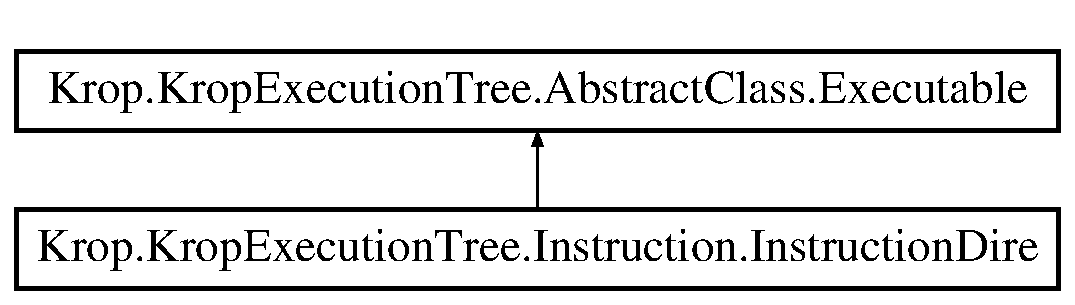
\includegraphics[height=2.000000cm]{class_krop_1_1_krop_execution_tree_1_1_instruction_1_1_instruction_dire}
\end{center}
\end{figure}
\subsection*{Public Member Functions}
\begin{DoxyCompactItemize}
\item 
\mbox{\hyperlink{class_krop_1_1_krop_execution_tree_1_1_instruction_1_1_instruction_dire_a5271ea25f2ef2b2a8b46db0b71efb3c7}{Instruction\+Dire}} (Node \+\_\+node\+Dire\+Statement, \mbox{\hyperlink{class_krop_1_1_krop_execution_tree_1_1_subprogram}{Subprogram}} \+\_\+parent\+Subprogram)
\item 
override bool \mbox{\hyperlink{class_krop_1_1_krop_execution_tree_1_1_instruction_1_1_instruction_dire_aef86c4e6b9ac3a4d17ed0c88db50a894}{Execute}} ()
\item 
void \mbox{\hyperlink{class_krop_1_1_krop_execution_tree_1_1_instruction_1_1_instruction_dire_adc2a2a8af353fbafe62bafc3e7116534}{Create\+Sentence}} (Node \+\_\+node\+Sentence)
\begin{DoxyCompactList}\small\item\em Set value = sentence \end{DoxyCompactList}\end{DoxyCompactItemize}


\subsection{Detailed Description}
Dire instruction 



\subsection{Constructor \& Destructor Documentation}
\mbox{\Hypertarget{class_krop_1_1_krop_execution_tree_1_1_instruction_1_1_instruction_dire_a5271ea25f2ef2b2a8b46db0b71efb3c7}\label{class_krop_1_1_krop_execution_tree_1_1_instruction_1_1_instruction_dire_a5271ea25f2ef2b2a8b46db0b71efb3c7}} 
\index{Krop\+::\+Krop\+Execution\+Tree\+::\+Instruction\+::\+Instruction\+Dire@{Krop\+::\+Krop\+Execution\+Tree\+::\+Instruction\+::\+Instruction\+Dire}!Instruction\+Dire@{Instruction\+Dire}}
\index{Instruction\+Dire@{Instruction\+Dire}!Krop\+::\+Krop\+Execution\+Tree\+::\+Instruction\+::\+Instruction\+Dire@{Krop\+::\+Krop\+Execution\+Tree\+::\+Instruction\+::\+Instruction\+Dire}}
\subsubsection{\texorpdfstring{Instruction\+Dire()}{InstructionDire()}}
{\footnotesize\ttfamily Krop.\+Krop\+Execution\+Tree.\+Instruction.\+Instruction\+Dire.\+Instruction\+Dire (\begin{DoxyParamCaption}\item[{Node}]{\+\_\+node\+Dire\+Statement,  }\item[{\mbox{\hyperlink{class_krop_1_1_krop_execution_tree_1_1_subprogram}{Subprogram}}}]{\+\_\+parent\+Subprogram }\end{DoxyParamCaption})}



\subsection{Member Function Documentation}
\mbox{\Hypertarget{class_krop_1_1_krop_execution_tree_1_1_instruction_1_1_instruction_dire_adc2a2a8af353fbafe62bafc3e7116534}\label{class_krop_1_1_krop_execution_tree_1_1_instruction_1_1_instruction_dire_adc2a2a8af353fbafe62bafc3e7116534}} 
\index{Krop\+::\+Krop\+Execution\+Tree\+::\+Instruction\+::\+Instruction\+Dire@{Krop\+::\+Krop\+Execution\+Tree\+::\+Instruction\+::\+Instruction\+Dire}!Create\+Sentence@{Create\+Sentence}}
\index{Create\+Sentence@{Create\+Sentence}!Krop\+::\+Krop\+Execution\+Tree\+::\+Instruction\+::\+Instruction\+Dire@{Krop\+::\+Krop\+Execution\+Tree\+::\+Instruction\+::\+Instruction\+Dire}}
\subsubsection{\texorpdfstring{Create\+Sentence()}{CreateSentence()}}
{\footnotesize\ttfamily void Krop.\+Krop\+Execution\+Tree.\+Instruction.\+Instruction\+Dire.\+Create\+Sentence (\begin{DoxyParamCaption}\item[{Node}]{\+\_\+node\+Sentence }\end{DoxyParamCaption})}



Set value = sentence 


\begin{DoxyParams}{Parameters}
{\em \+\_\+node\+Sentence} & Node containing the sentence\\
\hline
\end{DoxyParams}
\mbox{\Hypertarget{class_krop_1_1_krop_execution_tree_1_1_instruction_1_1_instruction_dire_aef86c4e6b9ac3a4d17ed0c88db50a894}\label{class_krop_1_1_krop_execution_tree_1_1_instruction_1_1_instruction_dire_aef86c4e6b9ac3a4d17ed0c88db50a894}} 
\index{Krop\+::\+Krop\+Execution\+Tree\+::\+Instruction\+::\+Instruction\+Dire@{Krop\+::\+Krop\+Execution\+Tree\+::\+Instruction\+::\+Instruction\+Dire}!Execute@{Execute}}
\index{Execute@{Execute}!Krop\+::\+Krop\+Execution\+Tree\+::\+Instruction\+::\+Instruction\+Dire@{Krop\+::\+Krop\+Execution\+Tree\+::\+Instruction\+::\+Instruction\+Dire}}
\subsubsection{\texorpdfstring{Execute()}{Execute()}}
{\footnotesize\ttfamily override bool Krop.\+Krop\+Execution\+Tree.\+Instruction.\+Instruction\+Dire.\+Execute (\begin{DoxyParamCaption}{ }\end{DoxyParamCaption})\hspace{0.3cm}{\ttfamily [virtual]}}



Implements \mbox{\hyperlink{class_krop_1_1_krop_execution_tree_1_1_abstract_class_1_1_executable_ac32692ce44b5f938a90111ee27e7b684}{Krop.\+Krop\+Execution\+Tree.\+Abstract\+Class.\+Executable}}.



The documentation for this class was generated from the following file\+:\begin{DoxyCompactItemize}
\item 
C\+:/\+Users/\+Stuart.\+G\+U\+E\+I\+S\+S\+A\+Z/\+Documents/\+Git\+Hub/\+Krop/\+Code/\+Krop/\+Krop\+Execution\+Tree/\+Instruction/\mbox{\hyperlink{_instruction_dire_8cs}{Instruction\+Dire.\+cs}}\end{DoxyCompactItemize}

\hypertarget{class_krop_1_1_krop_execution_tree_1_1_instruction_1_1_instruction_if}{}\section{Krop.\+Krop\+Execution\+Tree.\+Instruction.\+Instruction\+If Class Reference}
\label{class_krop_1_1_krop_execution_tree_1_1_instruction_1_1_instruction_if}\index{Krop.\+Krop\+Execution\+Tree.\+Instruction.\+Instruction\+If@{Krop.\+Krop\+Execution\+Tree.\+Instruction.\+Instruction\+If}}


If branching instruction  


Inheritance diagram for Krop.\+Krop\+Execution\+Tree.\+Instruction.\+Instruction\+If\+:\begin{figure}[H]
\begin{center}
\leavevmode
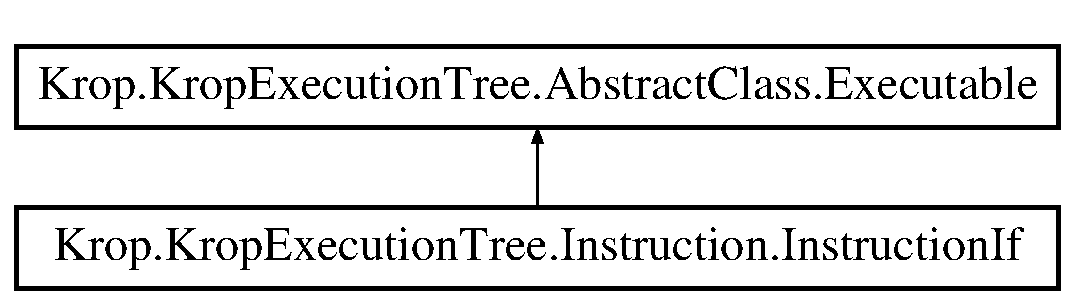
\includegraphics[height=2.000000cm]{class_krop_1_1_krop_execution_tree_1_1_instruction_1_1_instruction_if}
\end{center}
\end{figure}
\subsection*{Public Member Functions}
\begin{DoxyCompactItemize}
\item 
\mbox{\hyperlink{class_krop_1_1_krop_execution_tree_1_1_instruction_1_1_instruction_if_aa1e6065bcdd27ee97b616878b08ad745}{Instruction\+If}} (Node \+\_\+node\+If\+Else\+Statement, \mbox{\hyperlink{class_krop_1_1_krop_execution_tree_1_1_subprogram}{Subprogram}} \+\_\+parent\+Subprogram)
\item 
override bool \mbox{\hyperlink{class_krop_1_1_krop_execution_tree_1_1_instruction_1_1_instruction_if_a69ee340a90824643f703e28e2ab665a1}{Execute}} ()
\end{DoxyCompactItemize}
\subsection*{Public Attributes}
\begin{DoxyCompactItemize}
\item 
\mbox{\hyperlink{class_krop_1_1_krop_execution_tree_1_1_subprogram}{Subprogram}} \mbox{\hyperlink{class_krop_1_1_krop_execution_tree_1_1_instruction_1_1_instruction_if_ac302196115aed8fe5c9f79cb6a6d7747}{Parent\+Subprogram}}
\end{DoxyCompactItemize}


\subsection{Detailed Description}
If branching instruction 



\subsection{Constructor \& Destructor Documentation}
\mbox{\Hypertarget{class_krop_1_1_krop_execution_tree_1_1_instruction_1_1_instruction_if_aa1e6065bcdd27ee97b616878b08ad745}\label{class_krop_1_1_krop_execution_tree_1_1_instruction_1_1_instruction_if_aa1e6065bcdd27ee97b616878b08ad745}} 
\index{Krop\+::\+Krop\+Execution\+Tree\+::\+Instruction\+::\+Instruction\+If@{Krop\+::\+Krop\+Execution\+Tree\+::\+Instruction\+::\+Instruction\+If}!Instruction\+If@{Instruction\+If}}
\index{Instruction\+If@{Instruction\+If}!Krop\+::\+Krop\+Execution\+Tree\+::\+Instruction\+::\+Instruction\+If@{Krop\+::\+Krop\+Execution\+Tree\+::\+Instruction\+::\+Instruction\+If}}
\subsubsection{\texorpdfstring{Instruction\+If()}{InstructionIf()}}
{\footnotesize\ttfamily Krop.\+Krop\+Execution\+Tree.\+Instruction.\+Instruction\+If.\+Instruction\+If (\begin{DoxyParamCaption}\item[{Node}]{\+\_\+node\+If\+Else\+Statement,  }\item[{\mbox{\hyperlink{class_krop_1_1_krop_execution_tree_1_1_subprogram}{Subprogram}}}]{\+\_\+parent\+Subprogram }\end{DoxyParamCaption})}



\subsection{Member Function Documentation}
\mbox{\Hypertarget{class_krop_1_1_krop_execution_tree_1_1_instruction_1_1_instruction_if_a69ee340a90824643f703e28e2ab665a1}\label{class_krop_1_1_krop_execution_tree_1_1_instruction_1_1_instruction_if_a69ee340a90824643f703e28e2ab665a1}} 
\index{Krop\+::\+Krop\+Execution\+Tree\+::\+Instruction\+::\+Instruction\+If@{Krop\+::\+Krop\+Execution\+Tree\+::\+Instruction\+::\+Instruction\+If}!Execute@{Execute}}
\index{Execute@{Execute}!Krop\+::\+Krop\+Execution\+Tree\+::\+Instruction\+::\+Instruction\+If@{Krop\+::\+Krop\+Execution\+Tree\+::\+Instruction\+::\+Instruction\+If}}
\subsubsection{\texorpdfstring{Execute()}{Execute()}}
{\footnotesize\ttfamily override bool Krop.\+Krop\+Execution\+Tree.\+Instruction.\+Instruction\+If.\+Execute (\begin{DoxyParamCaption}{ }\end{DoxyParamCaption})\hspace{0.3cm}{\ttfamily [virtual]}}



Implements \mbox{\hyperlink{class_krop_1_1_krop_execution_tree_1_1_abstract_class_1_1_executable_ac32692ce44b5f938a90111ee27e7b684}{Krop.\+Krop\+Execution\+Tree.\+Abstract\+Class.\+Executable}}.



\subsection{Member Data Documentation}
\mbox{\Hypertarget{class_krop_1_1_krop_execution_tree_1_1_instruction_1_1_instruction_if_ac302196115aed8fe5c9f79cb6a6d7747}\label{class_krop_1_1_krop_execution_tree_1_1_instruction_1_1_instruction_if_ac302196115aed8fe5c9f79cb6a6d7747}} 
\index{Krop\+::\+Krop\+Execution\+Tree\+::\+Instruction\+::\+Instruction\+If@{Krop\+::\+Krop\+Execution\+Tree\+::\+Instruction\+::\+Instruction\+If}!Parent\+Subprogram@{Parent\+Subprogram}}
\index{Parent\+Subprogram@{Parent\+Subprogram}!Krop\+::\+Krop\+Execution\+Tree\+::\+Instruction\+::\+Instruction\+If@{Krop\+::\+Krop\+Execution\+Tree\+::\+Instruction\+::\+Instruction\+If}}
\subsubsection{\texorpdfstring{Parent\+Subprogram}{ParentSubprogram}}
{\footnotesize\ttfamily \mbox{\hyperlink{class_krop_1_1_krop_execution_tree_1_1_subprogram}{Subprogram}} Krop.\+Krop\+Execution\+Tree.\+Instruction.\+Instruction\+If.\+Parent\+Subprogram}



The documentation for this class was generated from the following file\+:\begin{DoxyCompactItemize}
\item 
C\+:/\+Users/\+Stuart.\+G\+U\+E\+I\+S\+S\+A\+Z/\+Documents/\+Git\+Hub/\+Krop/\+Code/\+Krop/\+Krop\+Execution\+Tree/\+Instruction/\mbox{\hyperlink{_instruction_if_8cs}{Instruction\+If.\+cs}}\end{DoxyCompactItemize}

\hypertarget{class_krop_1_1_krop_execution_tree_1_1_instruction_1_1_instruction_int}{}\section{Krop.\+Krop\+Execution\+Tree.\+Instruction.\+Instruction\+Int Class Reference}
\label{class_krop_1_1_krop_execution_tree_1_1_instruction_1_1_instruction_int}\index{Krop.\+Krop\+Execution\+Tree.\+Instruction.\+Instruction\+Int@{Krop.\+Krop\+Execution\+Tree.\+Instruction.\+Instruction\+Int}}


Declaration of an Int variable instruction  


Inheritance diagram for Krop.\+Krop\+Execution\+Tree.\+Instruction.\+Instruction\+Int\+:\begin{figure}[H]
\begin{center}
\leavevmode
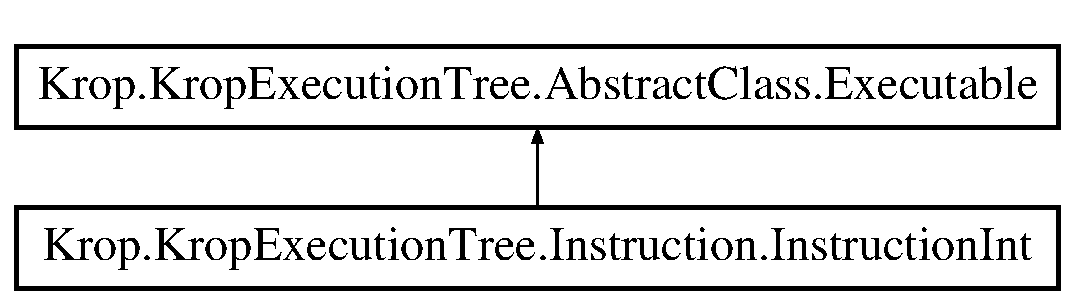
\includegraphics[height=2.000000cm]{class_krop_1_1_krop_execution_tree_1_1_instruction_1_1_instruction_int}
\end{center}
\end{figure}
\subsection*{Public Member Functions}
\begin{DoxyCompactItemize}
\item 
\mbox{\hyperlink{class_krop_1_1_krop_execution_tree_1_1_instruction_1_1_instruction_int_adb7584e305c335b0ba223dfa6316266e}{Instruction\+Int}} (Node \+\_\+node\+Int\+Statement, \mbox{\hyperlink{class_krop_1_1_krop_execution_tree_1_1_subprogram}{Subprogram}} \+\_\+parent\+Subprogram)
\item 
override bool \mbox{\hyperlink{class_krop_1_1_krop_execution_tree_1_1_instruction_1_1_instruction_int_ac2e3bee4e5a115c09e03815df9f6ae0e}{Execute}} ()
\end{DoxyCompactItemize}


\subsection{Detailed Description}
Declaration of an Int variable instruction 



\subsection{Constructor \& Destructor Documentation}
\mbox{\Hypertarget{class_krop_1_1_krop_execution_tree_1_1_instruction_1_1_instruction_int_adb7584e305c335b0ba223dfa6316266e}\label{class_krop_1_1_krop_execution_tree_1_1_instruction_1_1_instruction_int_adb7584e305c335b0ba223dfa6316266e}} 
\index{Krop\+::\+Krop\+Execution\+Tree\+::\+Instruction\+::\+Instruction\+Int@{Krop\+::\+Krop\+Execution\+Tree\+::\+Instruction\+::\+Instruction\+Int}!Instruction\+Int@{Instruction\+Int}}
\index{Instruction\+Int@{Instruction\+Int}!Krop\+::\+Krop\+Execution\+Tree\+::\+Instruction\+::\+Instruction\+Int@{Krop\+::\+Krop\+Execution\+Tree\+::\+Instruction\+::\+Instruction\+Int}}
\subsubsection{\texorpdfstring{Instruction\+Int()}{InstructionInt()}}
{\footnotesize\ttfamily Krop.\+Krop\+Execution\+Tree.\+Instruction.\+Instruction\+Int.\+Instruction\+Int (\begin{DoxyParamCaption}\item[{Node}]{\+\_\+node\+Int\+Statement,  }\item[{\mbox{\hyperlink{class_krop_1_1_krop_execution_tree_1_1_subprogram}{Subprogram}}}]{\+\_\+parent\+Subprogram }\end{DoxyParamCaption})}



\subsection{Member Function Documentation}
\mbox{\Hypertarget{class_krop_1_1_krop_execution_tree_1_1_instruction_1_1_instruction_int_ac2e3bee4e5a115c09e03815df9f6ae0e}\label{class_krop_1_1_krop_execution_tree_1_1_instruction_1_1_instruction_int_ac2e3bee4e5a115c09e03815df9f6ae0e}} 
\index{Krop\+::\+Krop\+Execution\+Tree\+::\+Instruction\+::\+Instruction\+Int@{Krop\+::\+Krop\+Execution\+Tree\+::\+Instruction\+::\+Instruction\+Int}!Execute@{Execute}}
\index{Execute@{Execute}!Krop\+::\+Krop\+Execution\+Tree\+::\+Instruction\+::\+Instruction\+Int@{Krop\+::\+Krop\+Execution\+Tree\+::\+Instruction\+::\+Instruction\+Int}}
\subsubsection{\texorpdfstring{Execute()}{Execute()}}
{\footnotesize\ttfamily override bool Krop.\+Krop\+Execution\+Tree.\+Instruction.\+Instruction\+Int.\+Execute (\begin{DoxyParamCaption}{ }\end{DoxyParamCaption})\hspace{0.3cm}{\ttfamily [virtual]}}



Implements \mbox{\hyperlink{class_krop_1_1_krop_execution_tree_1_1_abstract_class_1_1_executable_ac32692ce44b5f938a90111ee27e7b684}{Krop.\+Krop\+Execution\+Tree.\+Abstract\+Class.\+Executable}}.



The documentation for this class was generated from the following file\+:\begin{DoxyCompactItemize}
\item 
C\+:/\+Users/\+Stuart.\+G\+U\+E\+I\+S\+S\+A\+Z/\+Documents/\+Git\+Hub/\+Krop/\+Code/\+Krop/\+Krop\+Execution\+Tree/\+Instruction/\mbox{\hyperlink{_instruction_int_8cs}{Instruction\+Int.\+cs}}\end{DoxyCompactItemize}

\hypertarget{class_krop_1_1_krop_execution_tree_1_1_instruction_1_1_instruction_set_var}{}\section{Krop.\+Krop\+Execution\+Tree.\+Instruction.\+Instruction\+Set\+Var Class Reference}
\label{class_krop_1_1_krop_execution_tree_1_1_instruction_1_1_instruction_set_var}\index{Krop.\+Krop\+Execution\+Tree.\+Instruction.\+Instruction\+Set\+Var@{Krop.\+Krop\+Execution\+Tree.\+Instruction.\+Instruction\+Set\+Var}}


Set variable instruction  


Inheritance diagram for Krop.\+Krop\+Execution\+Tree.\+Instruction.\+Instruction\+Set\+Var\+:\begin{figure}[H]
\begin{center}
\leavevmode
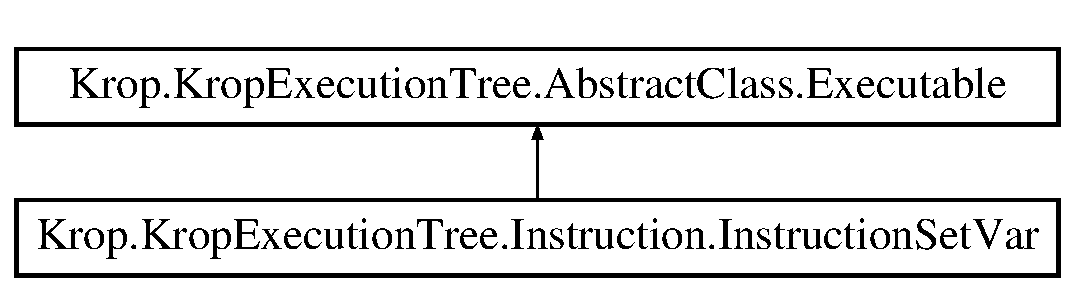
\includegraphics[height=2.000000cm]{class_krop_1_1_krop_execution_tree_1_1_instruction_1_1_instruction_set_var}
\end{center}
\end{figure}
\subsection*{Public Member Functions}
\begin{DoxyCompactItemize}
\item 
\mbox{\hyperlink{class_krop_1_1_krop_execution_tree_1_1_instruction_1_1_instruction_set_var_ae6382baf6329f3c178978ffc01c64ac5}{Instruction\+Set\+Var}} (Node \+\_\+node\+Int\+Statement, \mbox{\hyperlink{class_krop_1_1_krop_execution_tree_1_1_subprogram}{Subprogram}} \+\_\+parent\+Subprogram)
\item 
override bool \mbox{\hyperlink{class_krop_1_1_krop_execution_tree_1_1_instruction_1_1_instruction_set_var_a1c6739bcdc66cc9f50a8c9810958ed9f}{Execute}} ()
\end{DoxyCompactItemize}


\subsection{Detailed Description}
Set variable instruction 



\subsection{Constructor \& Destructor Documentation}
\mbox{\Hypertarget{class_krop_1_1_krop_execution_tree_1_1_instruction_1_1_instruction_set_var_ae6382baf6329f3c178978ffc01c64ac5}\label{class_krop_1_1_krop_execution_tree_1_1_instruction_1_1_instruction_set_var_ae6382baf6329f3c178978ffc01c64ac5}} 
\index{Krop\+::\+Krop\+Execution\+Tree\+::\+Instruction\+::\+Instruction\+Set\+Var@{Krop\+::\+Krop\+Execution\+Tree\+::\+Instruction\+::\+Instruction\+Set\+Var}!Instruction\+Set\+Var@{Instruction\+Set\+Var}}
\index{Instruction\+Set\+Var@{Instruction\+Set\+Var}!Krop\+::\+Krop\+Execution\+Tree\+::\+Instruction\+::\+Instruction\+Set\+Var@{Krop\+::\+Krop\+Execution\+Tree\+::\+Instruction\+::\+Instruction\+Set\+Var}}
\subsubsection{\texorpdfstring{Instruction\+Set\+Var()}{InstructionSetVar()}}
{\footnotesize\ttfamily Krop.\+Krop\+Execution\+Tree.\+Instruction.\+Instruction\+Set\+Var.\+Instruction\+Set\+Var (\begin{DoxyParamCaption}\item[{Node}]{\+\_\+node\+Int\+Statement,  }\item[{\mbox{\hyperlink{class_krop_1_1_krop_execution_tree_1_1_subprogram}{Subprogram}}}]{\+\_\+parent\+Subprogram }\end{DoxyParamCaption})}



\subsection{Member Function Documentation}
\mbox{\Hypertarget{class_krop_1_1_krop_execution_tree_1_1_instruction_1_1_instruction_set_var_a1c6739bcdc66cc9f50a8c9810958ed9f}\label{class_krop_1_1_krop_execution_tree_1_1_instruction_1_1_instruction_set_var_a1c6739bcdc66cc9f50a8c9810958ed9f}} 
\index{Krop\+::\+Krop\+Execution\+Tree\+::\+Instruction\+::\+Instruction\+Set\+Var@{Krop\+::\+Krop\+Execution\+Tree\+::\+Instruction\+::\+Instruction\+Set\+Var}!Execute@{Execute}}
\index{Execute@{Execute}!Krop\+::\+Krop\+Execution\+Tree\+::\+Instruction\+::\+Instruction\+Set\+Var@{Krop\+::\+Krop\+Execution\+Tree\+::\+Instruction\+::\+Instruction\+Set\+Var}}
\subsubsection{\texorpdfstring{Execute()}{Execute()}}
{\footnotesize\ttfamily override bool Krop.\+Krop\+Execution\+Tree.\+Instruction.\+Instruction\+Set\+Var.\+Execute (\begin{DoxyParamCaption}{ }\end{DoxyParamCaption})\hspace{0.3cm}{\ttfamily [virtual]}}



Implements \mbox{\hyperlink{class_krop_1_1_krop_execution_tree_1_1_abstract_class_1_1_executable_ac32692ce44b5f938a90111ee27e7b684}{Krop.\+Krop\+Execution\+Tree.\+Abstract\+Class.\+Executable}}.



The documentation for this class was generated from the following file\+:\begin{DoxyCompactItemize}
\item 
C\+:/\+Users/\+Stuart.\+G\+U\+E\+I\+S\+S\+A\+Z/\+Documents/\+Git\+Hub/\+Krop/\+Code/\+Krop/\+Krop\+Execution\+Tree/\+Instruction/\mbox{\hyperlink{_instruction_set_var_8cs}{Instruction\+Set\+Var.\+cs}}\end{DoxyCompactItemize}

\hypertarget{class_krop_1_1_krop_execution_tree_1_1_instruction_1_1_instruction_while}{}\section{Krop.\+Krop\+Execution\+Tree.\+Instruction.\+Instruction\+While Class Reference}
\label{class_krop_1_1_krop_execution_tree_1_1_instruction_1_1_instruction_while}\index{Krop.\+Krop\+Execution\+Tree.\+Instruction.\+Instruction\+While@{Krop.\+Krop\+Execution\+Tree.\+Instruction.\+Instruction\+While}}


While branching instruction  


Inheritance diagram for Krop.\+Krop\+Execution\+Tree.\+Instruction.\+Instruction\+While\+:\begin{figure}[H]
\begin{center}
\leavevmode
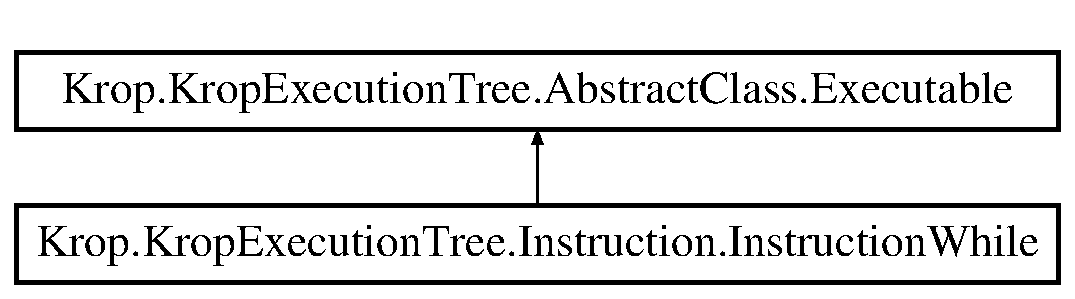
\includegraphics[height=2.000000cm]{class_krop_1_1_krop_execution_tree_1_1_instruction_1_1_instruction_while}
\end{center}
\end{figure}
\subsection*{Public Member Functions}
\begin{DoxyCompactItemize}
\item 
\mbox{\hyperlink{class_krop_1_1_krop_execution_tree_1_1_instruction_1_1_instruction_while_a5329f172e06824a1d611f92281c7b366}{Instruction\+While}} (Node \+\_\+node\+While\+Statement, \mbox{\hyperlink{class_krop_1_1_krop_execution_tree_1_1_subprogram}{Subprogram}} \+\_\+parent\+Subprogram)
\item 
override bool \mbox{\hyperlink{class_krop_1_1_krop_execution_tree_1_1_instruction_1_1_instruction_while_a98200d1758042e65604af4ad3cf95c9c}{Execute}} ()
\end{DoxyCompactItemize}
\subsection*{Public Attributes}
\begin{DoxyCompactItemize}
\item 
\mbox{\hyperlink{class_krop_1_1_krop_execution_tree_1_1_subprogram}{Subprogram}} \mbox{\hyperlink{class_krop_1_1_krop_execution_tree_1_1_instruction_1_1_instruction_while_ade7724a61c86599bdc632bfccc2363f4}{Parent\+Subprogram}}
\end{DoxyCompactItemize}


\subsection{Detailed Description}
While branching instruction 



\subsection{Constructor \& Destructor Documentation}
\mbox{\Hypertarget{class_krop_1_1_krop_execution_tree_1_1_instruction_1_1_instruction_while_a5329f172e06824a1d611f92281c7b366}\label{class_krop_1_1_krop_execution_tree_1_1_instruction_1_1_instruction_while_a5329f172e06824a1d611f92281c7b366}} 
\index{Krop\+::\+Krop\+Execution\+Tree\+::\+Instruction\+::\+Instruction\+While@{Krop\+::\+Krop\+Execution\+Tree\+::\+Instruction\+::\+Instruction\+While}!Instruction\+While@{Instruction\+While}}
\index{Instruction\+While@{Instruction\+While}!Krop\+::\+Krop\+Execution\+Tree\+::\+Instruction\+::\+Instruction\+While@{Krop\+::\+Krop\+Execution\+Tree\+::\+Instruction\+::\+Instruction\+While}}
\subsubsection{\texorpdfstring{Instruction\+While()}{InstructionWhile()}}
{\footnotesize\ttfamily Krop.\+Krop\+Execution\+Tree.\+Instruction.\+Instruction\+While.\+Instruction\+While (\begin{DoxyParamCaption}\item[{Node}]{\+\_\+node\+While\+Statement,  }\item[{\mbox{\hyperlink{class_krop_1_1_krop_execution_tree_1_1_subprogram}{Subprogram}}}]{\+\_\+parent\+Subprogram }\end{DoxyParamCaption})}



\subsection{Member Function Documentation}
\mbox{\Hypertarget{class_krop_1_1_krop_execution_tree_1_1_instruction_1_1_instruction_while_a98200d1758042e65604af4ad3cf95c9c}\label{class_krop_1_1_krop_execution_tree_1_1_instruction_1_1_instruction_while_a98200d1758042e65604af4ad3cf95c9c}} 
\index{Krop\+::\+Krop\+Execution\+Tree\+::\+Instruction\+::\+Instruction\+While@{Krop\+::\+Krop\+Execution\+Tree\+::\+Instruction\+::\+Instruction\+While}!Execute@{Execute}}
\index{Execute@{Execute}!Krop\+::\+Krop\+Execution\+Tree\+::\+Instruction\+::\+Instruction\+While@{Krop\+::\+Krop\+Execution\+Tree\+::\+Instruction\+::\+Instruction\+While}}
\subsubsection{\texorpdfstring{Execute()}{Execute()}}
{\footnotesize\ttfamily override bool Krop.\+Krop\+Execution\+Tree.\+Instruction.\+Instruction\+While.\+Execute (\begin{DoxyParamCaption}{ }\end{DoxyParamCaption})\hspace{0.3cm}{\ttfamily [virtual]}}



Implements \mbox{\hyperlink{class_krop_1_1_krop_execution_tree_1_1_abstract_class_1_1_executable_ac32692ce44b5f938a90111ee27e7b684}{Krop.\+Krop\+Execution\+Tree.\+Abstract\+Class.\+Executable}}.



\subsection{Member Data Documentation}
\mbox{\Hypertarget{class_krop_1_1_krop_execution_tree_1_1_instruction_1_1_instruction_while_ade7724a61c86599bdc632bfccc2363f4}\label{class_krop_1_1_krop_execution_tree_1_1_instruction_1_1_instruction_while_ade7724a61c86599bdc632bfccc2363f4}} 
\index{Krop\+::\+Krop\+Execution\+Tree\+::\+Instruction\+::\+Instruction\+While@{Krop\+::\+Krop\+Execution\+Tree\+::\+Instruction\+::\+Instruction\+While}!Parent\+Subprogram@{Parent\+Subprogram}}
\index{Parent\+Subprogram@{Parent\+Subprogram}!Krop\+::\+Krop\+Execution\+Tree\+::\+Instruction\+::\+Instruction\+While@{Krop\+::\+Krop\+Execution\+Tree\+::\+Instruction\+::\+Instruction\+While}}
\subsubsection{\texorpdfstring{Parent\+Subprogram}{ParentSubprogram}}
{\footnotesize\ttfamily \mbox{\hyperlink{class_krop_1_1_krop_execution_tree_1_1_subprogram}{Subprogram}} Krop.\+Krop\+Execution\+Tree.\+Instruction.\+Instruction\+While.\+Parent\+Subprogram}



The documentation for this class was generated from the following file\+:\begin{DoxyCompactItemize}
\item 
C\+:/\+Users/\+Stuart.\+G\+U\+E\+I\+S\+S\+A\+Z/\+Documents/\+Git\+Hub/\+Krop/\+Code/\+Krop/\+Krop\+Execution\+Tree/\+Instruction/\mbox{\hyperlink{_instruction_while_8cs}{Instruction\+While.\+cs}}\end{DoxyCompactItemize}

\hypertarget{class_krop_1_1_krop_execution_tree_1_1_variable_1_1_int_var}{}\section{Krop.\+Krop\+Execution\+Tree.\+Variable.\+Int\+Var Class Reference}
\label{class_krop_1_1_krop_execution_tree_1_1_variable_1_1_int_var}\index{Krop.\+Krop\+Execution\+Tree.\+Variable.\+Int\+Var@{Krop.\+Krop\+Execution\+Tree.\+Variable.\+Int\+Var}}


Hold an Int variable  


Inheritance diagram for Krop.\+Krop\+Execution\+Tree.\+Variable.\+Int\+Var\+:\begin{figure}[H]
\begin{center}
\leavevmode
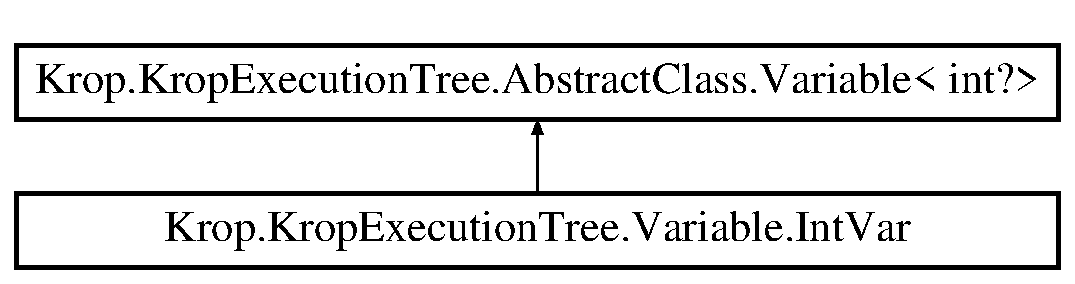
\includegraphics[height=2.000000cm]{class_krop_1_1_krop_execution_tree_1_1_variable_1_1_int_var}
\end{center}
\end{figure}
\subsection*{Public Member Functions}
\begin{DoxyCompactItemize}
\item 
\mbox{\hyperlink{class_krop_1_1_krop_execution_tree_1_1_variable_1_1_int_var_a9634bcdaa2d3d803ef3eb585e1533366}{Int\+Var}} (string \+\_\+name, int? \+\_\+value)
\item 
override string \mbox{\hyperlink{class_krop_1_1_krop_execution_tree_1_1_variable_1_1_int_var_ae48d754976bd6ed849a048ae209a689a}{Get\+Name}} ()
\begin{DoxyCompactList}\small\item\em Return variable name \end{DoxyCompactList}\item 
override int \mbox{\hyperlink{class_krop_1_1_krop_execution_tree_1_1_variable_1_1_int_var_a286e20f12bf8a03b9586596253a97144}{Get\+Value}} ()
\begin{DoxyCompactList}\small\item\em Return variable value \end{DoxyCompactList}\item 
override void \mbox{\hyperlink{class_krop_1_1_krop_execution_tree_1_1_variable_1_1_int_var_a437c24097ebfe4173e39880e76eb7d8b}{Set\+Value}} (int? \+\_\+value)
\begin{DoxyCompactList}\small\item\em Set variable value \end{DoxyCompactList}\item 
override string \mbox{\hyperlink{class_krop_1_1_krop_execution_tree_1_1_variable_1_1_int_var_acfe213da1e8d6fb0590872d3e7f9195b}{To\+String}} ()
\begin{DoxyCompactList}\small\item\em Return a string of the variable \end{DoxyCompactList}\end{DoxyCompactItemize}


\subsection{Detailed Description}
Hold an Int variable 



\subsection{Constructor \& Destructor Documentation}
\mbox{\Hypertarget{class_krop_1_1_krop_execution_tree_1_1_variable_1_1_int_var_a9634bcdaa2d3d803ef3eb585e1533366}\label{class_krop_1_1_krop_execution_tree_1_1_variable_1_1_int_var_a9634bcdaa2d3d803ef3eb585e1533366}} 
\index{Krop\+::\+Krop\+Execution\+Tree\+::\+Variable\+::\+Int\+Var@{Krop\+::\+Krop\+Execution\+Tree\+::\+Variable\+::\+Int\+Var}!Int\+Var@{Int\+Var}}
\index{Int\+Var@{Int\+Var}!Krop\+::\+Krop\+Execution\+Tree\+::\+Variable\+::\+Int\+Var@{Krop\+::\+Krop\+Execution\+Tree\+::\+Variable\+::\+Int\+Var}}
\subsubsection{\texorpdfstring{Int\+Var()}{IntVar()}}
{\footnotesize\ttfamily Krop.\+Krop\+Execution\+Tree.\+Variable.\+Int\+Var.\+Int\+Var (\begin{DoxyParamCaption}\item[{string}]{\+\_\+name,  }\item[{int?}]{\+\_\+value }\end{DoxyParamCaption})}



\subsection{Member Function Documentation}
\mbox{\Hypertarget{class_krop_1_1_krop_execution_tree_1_1_variable_1_1_int_var_ae48d754976bd6ed849a048ae209a689a}\label{class_krop_1_1_krop_execution_tree_1_1_variable_1_1_int_var_ae48d754976bd6ed849a048ae209a689a}} 
\index{Krop\+::\+Krop\+Execution\+Tree\+::\+Variable\+::\+Int\+Var@{Krop\+::\+Krop\+Execution\+Tree\+::\+Variable\+::\+Int\+Var}!Get\+Name@{Get\+Name}}
\index{Get\+Name@{Get\+Name}!Krop\+::\+Krop\+Execution\+Tree\+::\+Variable\+::\+Int\+Var@{Krop\+::\+Krop\+Execution\+Tree\+::\+Variable\+::\+Int\+Var}}
\subsubsection{\texorpdfstring{Get\+Name()}{GetName()}}
{\footnotesize\ttfamily override string Krop.\+Krop\+Execution\+Tree.\+Variable.\+Int\+Var.\+Get\+Name (\begin{DoxyParamCaption}{ }\end{DoxyParamCaption})\hspace{0.3cm}{\ttfamily [virtual]}}



Return variable name 

\begin{DoxyReturn}{Returns}
\mbox{\hyperlink{namespace_krop_1_1_krop_execution_tree_1_1_variable}{Variable}} name
\end{DoxyReturn}


Implements \mbox{\hyperlink{class_krop_1_1_krop_execution_tree_1_1_abstract_class_1_1_variable_a987550c24ebd0ceb01aec0b6edf51dfb}{Krop.\+Krop\+Execution\+Tree.\+Abstract\+Class.\+Variable$<$ int?$>$}}.

\mbox{\Hypertarget{class_krop_1_1_krop_execution_tree_1_1_variable_1_1_int_var_a286e20f12bf8a03b9586596253a97144}\label{class_krop_1_1_krop_execution_tree_1_1_variable_1_1_int_var_a286e20f12bf8a03b9586596253a97144}} 
\index{Krop\+::\+Krop\+Execution\+Tree\+::\+Variable\+::\+Int\+Var@{Krop\+::\+Krop\+Execution\+Tree\+::\+Variable\+::\+Int\+Var}!Get\+Value@{Get\+Value}}
\index{Get\+Value@{Get\+Value}!Krop\+::\+Krop\+Execution\+Tree\+::\+Variable\+::\+Int\+Var@{Krop\+::\+Krop\+Execution\+Tree\+::\+Variable\+::\+Int\+Var}}
\subsubsection{\texorpdfstring{Get\+Value()}{GetValue()}}
{\footnotesize\ttfamily override int Krop.\+Krop\+Execution\+Tree.\+Variable.\+Int\+Var.\+Get\+Value (\begin{DoxyParamCaption}{ }\end{DoxyParamCaption})\hspace{0.3cm}{\ttfamily [virtual]}}



Return variable value 

\begin{DoxyReturn}{Returns}
\mbox{\hyperlink{namespace_krop_1_1_krop_execution_tree_1_1_variable}{Variable}} value
\end{DoxyReturn}


Implements \mbox{\hyperlink{class_krop_1_1_krop_execution_tree_1_1_abstract_class_1_1_variable_a9d77d99b187893c15c5847ffa6fe0daf}{Krop.\+Krop\+Execution\+Tree.\+Abstract\+Class.\+Variable$<$ int?$>$}}.

\mbox{\Hypertarget{class_krop_1_1_krop_execution_tree_1_1_variable_1_1_int_var_a437c24097ebfe4173e39880e76eb7d8b}\label{class_krop_1_1_krop_execution_tree_1_1_variable_1_1_int_var_a437c24097ebfe4173e39880e76eb7d8b}} 
\index{Krop\+::\+Krop\+Execution\+Tree\+::\+Variable\+::\+Int\+Var@{Krop\+::\+Krop\+Execution\+Tree\+::\+Variable\+::\+Int\+Var}!Set\+Value@{Set\+Value}}
\index{Set\+Value@{Set\+Value}!Krop\+::\+Krop\+Execution\+Tree\+::\+Variable\+::\+Int\+Var@{Krop\+::\+Krop\+Execution\+Tree\+::\+Variable\+::\+Int\+Var}}
\subsubsection{\texorpdfstring{Set\+Value()}{SetValue()}}
{\footnotesize\ttfamily override void Krop.\+Krop\+Execution\+Tree.\+Variable.\+Int\+Var.\+Set\+Value (\begin{DoxyParamCaption}\item[{int?}]{\+\_\+value }\end{DoxyParamCaption})}



Set variable value 


\begin{DoxyParams}{Parameters}
{\em \+\_\+value} & Value\\
\hline
\end{DoxyParams}
\mbox{\Hypertarget{class_krop_1_1_krop_execution_tree_1_1_variable_1_1_int_var_acfe213da1e8d6fb0590872d3e7f9195b}\label{class_krop_1_1_krop_execution_tree_1_1_variable_1_1_int_var_acfe213da1e8d6fb0590872d3e7f9195b}} 
\index{Krop\+::\+Krop\+Execution\+Tree\+::\+Variable\+::\+Int\+Var@{Krop\+::\+Krop\+Execution\+Tree\+::\+Variable\+::\+Int\+Var}!To\+String@{To\+String}}
\index{To\+String@{To\+String}!Krop\+::\+Krop\+Execution\+Tree\+::\+Variable\+::\+Int\+Var@{Krop\+::\+Krop\+Execution\+Tree\+::\+Variable\+::\+Int\+Var}}
\subsubsection{\texorpdfstring{To\+String()}{ToString()}}
{\footnotesize\ttfamily override string Krop.\+Krop\+Execution\+Tree.\+Variable.\+Int\+Var.\+To\+String (\begin{DoxyParamCaption}{ }\end{DoxyParamCaption})\hspace{0.3cm}{\ttfamily [virtual]}}



Return a string of the variable 

\begin{DoxyReturn}{Returns}
String variable
\end{DoxyReturn}


Implements \mbox{\hyperlink{class_krop_1_1_krop_execution_tree_1_1_abstract_class_1_1_variable_ae78ccbb029efb966e1edff0ae101f367}{Krop.\+Krop\+Execution\+Tree.\+Abstract\+Class.\+Variable$<$ int?$>$}}.



The documentation for this class was generated from the following file\+:\begin{DoxyCompactItemize}
\item 
C\+:/\+Users/\+Stuart.\+G\+U\+E\+I\+S\+S\+A\+Z/\+Documents/\+Git\+Hub/\+Krop/\+Code/\+Krop/\+Krop\+Execution\+Tree/\+Variable/\mbox{\hyperlink{_int_var_8cs}{Int\+Var.\+cs}}\end{DoxyCompactItemize}

\hypertarget{interface_krop_1_1_krop_execution_tree_1_1_interface_1_1_i_variable}{}\section{Krop.\+Krop\+Execution\+Tree.\+Interface.\+I\+Variable Interface Reference}
\label{interface_krop_1_1_krop_execution_tree_1_1_interface_1_1_i_variable}\index{Krop.\+Krop\+Execution\+Tree.\+Interface.\+I\+Variable@{Krop.\+Krop\+Execution\+Tree.\+Interface.\+I\+Variable}}


\mbox{\hyperlink{namespace_krop_1_1_krop_execution_tree_1_1_variable}{Variable}} interface  


Inheritance diagram for Krop.\+Krop\+Execution\+Tree.\+Interface.\+I\+Variable\+:\begin{figure}[H]
\begin{center}
\leavevmode
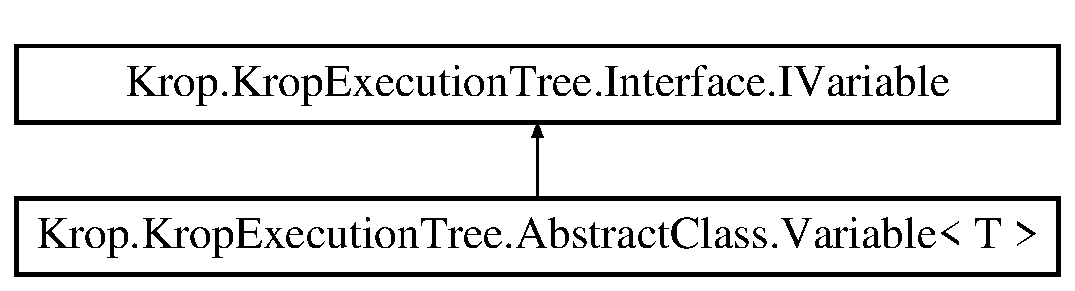
\includegraphics[height=2.000000cm]{interface_krop_1_1_krop_execution_tree_1_1_interface_1_1_i_variable}
\end{center}
\end{figure}
\subsection*{Public Member Functions}
\begin{DoxyCompactItemize}
\item 
string \mbox{\hyperlink{interface_krop_1_1_krop_execution_tree_1_1_interface_1_1_i_variable_a0a1ca374f3af72c44d0754c00e8c26d3}{Get\+Name}} ()
\item 
string \mbox{\hyperlink{interface_krop_1_1_krop_execution_tree_1_1_interface_1_1_i_variable_a4d3f36256ae24e2550ee0a16d3142822}{To\+String}} ()
\end{DoxyCompactItemize}


\subsection{Detailed Description}
\mbox{\hyperlink{namespace_krop_1_1_krop_execution_tree_1_1_variable}{Variable}} interface 



\subsection{Member Function Documentation}
\mbox{\Hypertarget{interface_krop_1_1_krop_execution_tree_1_1_interface_1_1_i_variable_a0a1ca374f3af72c44d0754c00e8c26d3}\label{interface_krop_1_1_krop_execution_tree_1_1_interface_1_1_i_variable_a0a1ca374f3af72c44d0754c00e8c26d3}} 
\index{Krop\+::\+Krop\+Execution\+Tree\+::\+Interface\+::\+I\+Variable@{Krop\+::\+Krop\+Execution\+Tree\+::\+Interface\+::\+I\+Variable}!Get\+Name@{Get\+Name}}
\index{Get\+Name@{Get\+Name}!Krop\+::\+Krop\+Execution\+Tree\+::\+Interface\+::\+I\+Variable@{Krop\+::\+Krop\+Execution\+Tree\+::\+Interface\+::\+I\+Variable}}
\subsubsection{\texorpdfstring{Get\+Name()}{GetName()}}
{\footnotesize\ttfamily string Krop.\+Krop\+Execution\+Tree.\+Interface.\+I\+Variable.\+Get\+Name (\begin{DoxyParamCaption}{ }\end{DoxyParamCaption})}



Implemented in \mbox{\hyperlink{class_krop_1_1_krop_execution_tree_1_1_abstract_class_1_1_variable_a987550c24ebd0ceb01aec0b6edf51dfb}{Krop.\+Krop\+Execution\+Tree.\+Abstract\+Class.\+Variable$<$ T $>$}}.

\mbox{\Hypertarget{interface_krop_1_1_krop_execution_tree_1_1_interface_1_1_i_variable_a4d3f36256ae24e2550ee0a16d3142822}\label{interface_krop_1_1_krop_execution_tree_1_1_interface_1_1_i_variable_a4d3f36256ae24e2550ee0a16d3142822}} 
\index{Krop\+::\+Krop\+Execution\+Tree\+::\+Interface\+::\+I\+Variable@{Krop\+::\+Krop\+Execution\+Tree\+::\+Interface\+::\+I\+Variable}!To\+String@{To\+String}}
\index{To\+String@{To\+String}!Krop\+::\+Krop\+Execution\+Tree\+::\+Interface\+::\+I\+Variable@{Krop\+::\+Krop\+Execution\+Tree\+::\+Interface\+::\+I\+Variable}}
\subsubsection{\texorpdfstring{To\+String()}{ToString()}}
{\footnotesize\ttfamily string Krop.\+Krop\+Execution\+Tree.\+Interface.\+I\+Variable.\+To\+String (\begin{DoxyParamCaption}{ }\end{DoxyParamCaption})}



Implemented in \mbox{\hyperlink{class_krop_1_1_krop_execution_tree_1_1_abstract_class_1_1_variable_ae78ccbb029efb966e1edff0ae101f367}{Krop.\+Krop\+Execution\+Tree.\+Abstract\+Class.\+Variable$<$ T $>$}}.



The documentation for this interface was generated from the following file\+:\begin{DoxyCompactItemize}
\item 
C\+:/\+Users/\+Stuart.\+G\+U\+E\+I\+S\+S\+A\+Z/\+Documents/\+Git\+Hub/\+Krop/\+Code/\+Krop/\+Krop\+Execution\+Tree/\+Interface/\mbox{\hyperlink{_i_variable_8cs}{I\+Variable.\+cs}}\end{DoxyCompactItemize}

\hypertarget{struct_krop_1_1_krohonde_1_1_level}{}\section{Krop.\+Krohonde.\+Level Struct Reference}
\label{struct_krop_1_1_krohonde_1_1_level}\index{Krop.\+Krohonde.\+Level@{Krop.\+Krohonde.\+Level}}
\subsection*{Public Member Functions}
\begin{DoxyCompactItemize}
\item 
\mbox{\hyperlink{struct_krop_1_1_krohonde_1_1_level_aac39539c546fa2284e8ff762b4898c98}{Level}} (int width, int height)
\begin{DoxyCompactList}\small\item\em Load the default garden \end{DoxyCompactList}\item 
\mbox{\hyperlink{struct_krop_1_1_krohonde_1_1_level_a1e442ecde4d1692da04bb530c451d421}{Level}} (string file\+Path)
\begin{DoxyCompactList}\small\item\em Load the selected garden \end{DoxyCompactList}\end{DoxyCompactItemize}
\subsection*{Properties}
\begin{DoxyCompactItemize}
\item 
int \mbox{\hyperlink{struct_krop_1_1_krohonde_1_1_level_a44e520a8301e4f9d46b1b0feee4a7e9d}{Width}}\hspace{0.3cm}{\ttfamily  \mbox{[}get\mbox{]}}
\item 
int \mbox{\hyperlink{struct_krop_1_1_krohonde_1_1_level_a9a6ee04aee1439f061009af27688d39f}{Height}}\hspace{0.3cm}{\ttfamily  \mbox{[}get\mbox{]}}
\item 
string \mbox{\hyperlink{struct_krop_1_1_krohonde_1_1_level_a13ed09516431dcc51e4ee6dad01afdb1}{File\+Path}}\hspace{0.3cm}{\ttfamily  \mbox{[}get\mbox{]}}
\item 
\mbox{\hyperlink{struct_krop_1_1_krohonde_1_1_block}{Block}} \mbox{\hyperlink{struct_krop_1_1_krohonde_1_1_level_aa12f79d6846914cf1ed7dcd7f5d99f70}{this\mbox{[}int \+\_\+pos\+X, int \+\_\+pos\+Y\mbox{]}}}\hspace{0.3cm}{\ttfamily  \mbox{[}get, set\mbox{]}}
\end{DoxyCompactItemize}


\subsection{Constructor \& Destructor Documentation}
\mbox{\Hypertarget{struct_krop_1_1_krohonde_1_1_level_aac39539c546fa2284e8ff762b4898c98}\label{struct_krop_1_1_krohonde_1_1_level_aac39539c546fa2284e8ff762b4898c98}} 
\index{Krop\+::\+Krohonde\+::\+Level@{Krop\+::\+Krohonde\+::\+Level}!Level@{Level}}
\index{Level@{Level}!Krop\+::\+Krohonde\+::\+Level@{Krop\+::\+Krohonde\+::\+Level}}
\subsubsection{\texorpdfstring{Level()}{Level()}\hspace{0.1cm}{\footnotesize\ttfamily [1/2]}}
{\footnotesize\ttfamily Krop.\+Krohonde.\+Level.\+Level (\begin{DoxyParamCaption}\item[{int}]{width,  }\item[{int}]{height }\end{DoxyParamCaption})}



Load the default garden 


\begin{DoxyParams}{Parameters}
{\em width} & \\
\hline
{\em height} & \\
\hline
\end{DoxyParams}
\mbox{\Hypertarget{struct_krop_1_1_krohonde_1_1_level_a1e442ecde4d1692da04bb530c451d421}\label{struct_krop_1_1_krohonde_1_1_level_a1e442ecde4d1692da04bb530c451d421}} 
\index{Krop\+::\+Krohonde\+::\+Level@{Krop\+::\+Krohonde\+::\+Level}!Level@{Level}}
\index{Level@{Level}!Krop\+::\+Krohonde\+::\+Level@{Krop\+::\+Krohonde\+::\+Level}}
\subsubsection{\texorpdfstring{Level()}{Level()}\hspace{0.1cm}{\footnotesize\ttfamily [2/2]}}
{\footnotesize\ttfamily Krop.\+Krohonde.\+Level.\+Level (\begin{DoxyParamCaption}\item[{string}]{file\+Path }\end{DoxyParamCaption})}



Load the selected garden 


\begin{DoxyParams}{Parameters}
{\em file\+Path} & \\
\hline
\end{DoxyParams}


\subsection{Property Documentation}
\mbox{\Hypertarget{struct_krop_1_1_krohonde_1_1_level_a13ed09516431dcc51e4ee6dad01afdb1}\label{struct_krop_1_1_krohonde_1_1_level_a13ed09516431dcc51e4ee6dad01afdb1}} 
\index{Krop\+::\+Krohonde\+::\+Level@{Krop\+::\+Krohonde\+::\+Level}!File\+Path@{File\+Path}}
\index{File\+Path@{File\+Path}!Krop\+::\+Krohonde\+::\+Level@{Krop\+::\+Krohonde\+::\+Level}}
\subsubsection{\texorpdfstring{File\+Path}{FilePath}}
{\footnotesize\ttfamily string Krop.\+Krohonde.\+Level.\+File\+Path\hspace{0.3cm}{\ttfamily [get]}}

\mbox{\Hypertarget{struct_krop_1_1_krohonde_1_1_level_a9a6ee04aee1439f061009af27688d39f}\label{struct_krop_1_1_krohonde_1_1_level_a9a6ee04aee1439f061009af27688d39f}} 
\index{Krop\+::\+Krohonde\+::\+Level@{Krop\+::\+Krohonde\+::\+Level}!Height@{Height}}
\index{Height@{Height}!Krop\+::\+Krohonde\+::\+Level@{Krop\+::\+Krohonde\+::\+Level}}
\subsubsection{\texorpdfstring{Height}{Height}}
{\footnotesize\ttfamily int Krop.\+Krohonde.\+Level.\+Height\hspace{0.3cm}{\ttfamily [get]}}

\mbox{\Hypertarget{struct_krop_1_1_krohonde_1_1_level_aa12f79d6846914cf1ed7dcd7f5d99f70}\label{struct_krop_1_1_krohonde_1_1_level_aa12f79d6846914cf1ed7dcd7f5d99f70}} 
\index{Krop\+::\+Krohonde\+::\+Level@{Krop\+::\+Krohonde\+::\+Level}!this\mbox{[}int \+\_\+pos\+X, int \+\_\+posY\mbox{]}@{this[int \+\_\+pos\+X, int \+\_\+posY]}}
\index{this\mbox{[}int \+\_\+pos\+X, int \+\_\+posY\mbox{]}@{this[int \+\_\+pos\+X, int \+\_\+posY]}!Krop\+::\+Krohonde\+::\+Level@{Krop\+::\+Krohonde\+::\+Level}}
\subsubsection{\texorpdfstring{this[int \+\_\+pos\+X, int \+\_\+posY]}{this[int \_posX, int \_posY]}}
{\footnotesize\ttfamily \mbox{\hyperlink{struct_krop_1_1_krohonde_1_1_block}{Block}} Krop.\+Krohonde.\+Level.\+this\mbox{[}int \+\_\+posX, int \+\_\+posY\mbox{]}\hspace{0.3cm}{\ttfamily [get]}, {\ttfamily [set]}}

\mbox{\Hypertarget{struct_krop_1_1_krohonde_1_1_level_a44e520a8301e4f9d46b1b0feee4a7e9d}\label{struct_krop_1_1_krohonde_1_1_level_a44e520a8301e4f9d46b1b0feee4a7e9d}} 
\index{Krop\+::\+Krohonde\+::\+Level@{Krop\+::\+Krohonde\+::\+Level}!Width@{Width}}
\index{Width@{Width}!Krop\+::\+Krohonde\+::\+Level@{Krop\+::\+Krohonde\+::\+Level}}
\subsubsection{\texorpdfstring{Width}{Width}}
{\footnotesize\ttfamily int Krop.\+Krohonde.\+Level.\+Width\hspace{0.3cm}{\ttfamily [get]}}



The documentation for this struct was generated from the following file\+:\begin{DoxyCompactItemize}
\item 
C\+:/\+Users/\+Stuart.\+G\+U\+E\+I\+S\+S\+A\+Z/\+Documents/\+Git\+Hub/\+Krop/\+Code/\+Krop/\+Krohonde/\mbox{\hyperlink{_level_8cs}{Level.\+cs}}\end{DoxyCompactItemize}

\hypertarget{class_krop_1_1_krop_execution_tree_1_1_abstract_class_1_1_measurable}{}\section{Krop.\+Krop\+Execution\+Tree.\+Abstract\+Class.\+Measurable$<$ T $>$ Class Template Reference}
\label{class_krop_1_1_krop_execution_tree_1_1_abstract_class_1_1_measurable}\index{Krop.\+Krop\+Execution\+Tree.\+Abstract\+Class.\+Measurable$<$ T $>$@{Krop.\+Krop\+Execution\+Tree.\+Abstract\+Class.\+Measurable$<$ T $>$}}


\mbox{\hyperlink{class_krop_1_1_krop_execution_tree_1_1_abstract_class_1_1_measurable}{Measurable}} objects represent expressions that can be computed. The result of the computation is of type T  


\subsection*{Public Member Functions}
\begin{DoxyCompactItemize}
\item 
abstract T \mbox{\hyperlink{class_krop_1_1_krop_execution_tree_1_1_abstract_class_1_1_measurable_afe91c739e2db11c8f316b07e8f55f7bb}{Evaluate}} ()
\begin{DoxyCompactList}\small\item\em Trigger the computation of the expression \end{DoxyCompactList}\item 
bool \mbox{\hyperlink{class_krop_1_1_krop_execution_tree_1_1_abstract_class_1_1_measurable_af2cf52c10abba40adf7a4abd355d9c04}{Can\+Evaluate}} ()
\begin{DoxyCompactList}\small\item\em Wait ending previous order \end{DoxyCompactList}\end{DoxyCompactItemize}


\subsection{Detailed Description}
\mbox{\hyperlink{class_krop_1_1_krop_execution_tree_1_1_abstract_class_1_1_measurable}{Measurable}} objects represent expressions that can be computed. The result of the computation is of type T 



\subsection{Member Function Documentation}
\mbox{\Hypertarget{class_krop_1_1_krop_execution_tree_1_1_abstract_class_1_1_measurable_af2cf52c10abba40adf7a4abd355d9c04}\label{class_krop_1_1_krop_execution_tree_1_1_abstract_class_1_1_measurable_af2cf52c10abba40adf7a4abd355d9c04}} 
\index{Krop\+::\+Krop\+Execution\+Tree\+::\+Abstract\+Class\+::\+Measurable@{Krop\+::\+Krop\+Execution\+Tree\+::\+Abstract\+Class\+::\+Measurable}!Can\+Evaluate@{Can\+Evaluate}}
\index{Can\+Evaluate@{Can\+Evaluate}!Krop\+::\+Krop\+Execution\+Tree\+::\+Abstract\+Class\+::\+Measurable@{Krop\+::\+Krop\+Execution\+Tree\+::\+Abstract\+Class\+::\+Measurable}}
\subsubsection{\texorpdfstring{Can\+Evaluate()}{CanEvaluate()}}
{\footnotesize\ttfamily bool \mbox{\hyperlink{class_krop_1_1_krop_execution_tree_1_1_abstract_class_1_1_measurable}{Krop.\+Krop\+Execution\+Tree.\+Abstract\+Class.\+Measurable}}$<$ T $>$.Can\+Evaluate (\begin{DoxyParamCaption}{ }\end{DoxyParamCaption})}



Wait ending previous order 

\begin{DoxyReturn}{Returns}

\end{DoxyReturn}
\mbox{\Hypertarget{class_krop_1_1_krop_execution_tree_1_1_abstract_class_1_1_measurable_afe91c739e2db11c8f316b07e8f55f7bb}\label{class_krop_1_1_krop_execution_tree_1_1_abstract_class_1_1_measurable_afe91c739e2db11c8f316b07e8f55f7bb}} 
\index{Krop\+::\+Krop\+Execution\+Tree\+::\+Abstract\+Class\+::\+Measurable@{Krop\+::\+Krop\+Execution\+Tree\+::\+Abstract\+Class\+::\+Measurable}!Evaluate@{Evaluate}}
\index{Evaluate@{Evaluate}!Krop\+::\+Krop\+Execution\+Tree\+::\+Abstract\+Class\+::\+Measurable@{Krop\+::\+Krop\+Execution\+Tree\+::\+Abstract\+Class\+::\+Measurable}}
\subsubsection{\texorpdfstring{Evaluate()}{Evaluate()}}
{\footnotesize\ttfamily abstract T \mbox{\hyperlink{class_krop_1_1_krop_execution_tree_1_1_abstract_class_1_1_measurable}{Krop.\+Krop\+Execution\+Tree.\+Abstract\+Class.\+Measurable}}$<$ T $>$.Evaluate (\begin{DoxyParamCaption}{ }\end{DoxyParamCaption})\hspace{0.3cm}{\ttfamily [pure virtual]}}



Trigger the computation of the expression 

\begin{DoxyReturn}{Returns}
The result of the computation 
\end{DoxyReturn}


Implemented in \mbox{\hyperlink{class_krop_1_1_krop_execution_tree_1_1_condition_1_1_boolean_expression_a0d5dccaa10e9fa7933cf96edd1e670dd}{Krop.\+Krop\+Execution\+Tree.\+Condition.\+Boolean\+Expression}}, \mbox{\hyperlink{class_krop_1_1_krop_execution_tree_1_1_condition_1_1_boolean_function_a1e274ef1079b4ab8136c45b5f48c747e}{Krop.\+Krop\+Execution\+Tree.\+Condition.\+Boolean\+Function}}, and \mbox{\hyperlink{class_krop_1_1_krop_execution_tree_1_1_condition_1_1_boolean_var_a293790e0485139dcf84fe9c35a5bac4a}{Krop.\+Krop\+Execution\+Tree.\+Condition.\+Boolean\+Var}}.



The documentation for this class was generated from the following file\+:\begin{DoxyCompactItemize}
\item 
C\+:/\+Users/\+Stuart.\+G\+U\+E\+I\+S\+S\+A\+Z/\+Documents/\+Git\+Hub/\+Krop/\+Code/\+Krop/\+Krop\+Execution\+Tree/\+Abstract\+Class/\mbox{\hyperlink{_measurable_8cs}{Measurable.\+cs}}\end{DoxyCompactItemize}

\hypertarget{class_krop_1_1_krohonde_1_1_spritebatch}{}\section{Krop.\+Krohonde.\+Spritebatch Class Reference}
\label{class_krop_1_1_krohonde_1_1_spritebatch}\index{Krop.\+Krohonde.\+Spritebatch@{Krop.\+Krohonde.\+Spritebatch}}
\subsection*{Static Public Member Functions}
\begin{DoxyCompactItemize}
\item 
static void \mbox{\hyperlink{class_krop_1_1_krohonde_1_1_spritebatch_af312141beabae3816e190343bb63b1ee}{Draw\+Sprite}} (\mbox{\hyperlink{class_krop_1_1_krohonde_1_1_texture2_d}{Texture2D}} texture, RectangleF rectangle)
\item 
static void \mbox{\hyperlink{class_krop_1_1_krohonde_1_1_spritebatch_a0edfdfb7ac4997f89578c617b2f9da53}{Draw\+Sprite}} (\mbox{\hyperlink{class_krop_1_1_krohonde_1_1_texture2_d}{Texture2D}} texture, RectangleF rectangle, Color color, RectangleF? source\+Rec=null)
\item 
static void \mbox{\hyperlink{class_krop_1_1_krohonde_1_1_spritebatch_a6e80cba942888ba405410ce5361b550c}{Draw\+Sprite}} (\mbox{\hyperlink{class_krop_1_1_krohonde_1_1_texture2_d}{Texture2D}} texture, Vector2 position)
\item 
static void \mbox{\hyperlink{class_krop_1_1_krohonde_1_1_spritebatch_ab4a2ef07acfe42c03b8de094bd499197}{Draw\+Sprite}} (\mbox{\hyperlink{class_krop_1_1_krohonde_1_1_texture2_d}{Texture2D}} texture, Vector2 position, Vector2 scale)
\item 
static void \mbox{\hyperlink{class_krop_1_1_krohonde_1_1_spritebatch_a1c7dd22c521c29636044af5194c846a0}{Draw\+Sprite}} (\mbox{\hyperlink{class_krop_1_1_krohonde_1_1_texture2_d}{Texture2D}} texture, Vector2 position, Vector2 scale, Color color)
\item 
static void \mbox{\hyperlink{class_krop_1_1_krohonde_1_1_spritebatch_a68b5800b1626fa035e66b7b40badc245}{Draw\+Sprite}} (\mbox{\hyperlink{class_krop_1_1_krohonde_1_1_texture2_d}{Texture2D}} texture, Vector2 position, Vector2 scale, Color color, Vector2 origin, RectangleF? source\+Rec=null)
\item 
static void \mbox{\hyperlink{class_krop_1_1_krohonde_1_1_spritebatch_acee872767762886ac0b07fd3f645205e}{Begin}} (int screen\+Width, int screen\+Height)
\end{DoxyCompactItemize}


\subsection{Member Function Documentation}
\mbox{\Hypertarget{class_krop_1_1_krohonde_1_1_spritebatch_acee872767762886ac0b07fd3f645205e}\label{class_krop_1_1_krohonde_1_1_spritebatch_acee872767762886ac0b07fd3f645205e}} 
\index{Krop\+::\+Krohonde\+::\+Spritebatch@{Krop\+::\+Krohonde\+::\+Spritebatch}!Begin@{Begin}}
\index{Begin@{Begin}!Krop\+::\+Krohonde\+::\+Spritebatch@{Krop\+::\+Krohonde\+::\+Spritebatch}}
\subsubsection{\texorpdfstring{Begin()}{Begin()}}
{\footnotesize\ttfamily static void Krop.\+Krohonde.\+Spritebatch.\+Begin (\begin{DoxyParamCaption}\item[{int}]{screen\+Width,  }\item[{int}]{screen\+Height }\end{DoxyParamCaption})\hspace{0.3cm}{\ttfamily [static]}}

\mbox{\Hypertarget{class_krop_1_1_krohonde_1_1_spritebatch_af312141beabae3816e190343bb63b1ee}\label{class_krop_1_1_krohonde_1_1_spritebatch_af312141beabae3816e190343bb63b1ee}} 
\index{Krop\+::\+Krohonde\+::\+Spritebatch@{Krop\+::\+Krohonde\+::\+Spritebatch}!Draw\+Sprite@{Draw\+Sprite}}
\index{Draw\+Sprite@{Draw\+Sprite}!Krop\+::\+Krohonde\+::\+Spritebatch@{Krop\+::\+Krohonde\+::\+Spritebatch}}
\subsubsection{\texorpdfstring{Draw\+Sprite()}{DrawSprite()}\hspace{0.1cm}{\footnotesize\ttfamily [1/6]}}
{\footnotesize\ttfamily static void Krop.\+Krohonde.\+Spritebatch.\+Draw\+Sprite (\begin{DoxyParamCaption}\item[{\mbox{\hyperlink{class_krop_1_1_krohonde_1_1_texture2_d}{Texture2D}}}]{texture,  }\item[{RectangleF}]{rectangle }\end{DoxyParamCaption})\hspace{0.3cm}{\ttfamily [static]}}

\mbox{\Hypertarget{class_krop_1_1_krohonde_1_1_spritebatch_a0edfdfb7ac4997f89578c617b2f9da53}\label{class_krop_1_1_krohonde_1_1_spritebatch_a0edfdfb7ac4997f89578c617b2f9da53}} 
\index{Krop\+::\+Krohonde\+::\+Spritebatch@{Krop\+::\+Krohonde\+::\+Spritebatch}!Draw\+Sprite@{Draw\+Sprite}}
\index{Draw\+Sprite@{Draw\+Sprite}!Krop\+::\+Krohonde\+::\+Spritebatch@{Krop\+::\+Krohonde\+::\+Spritebatch}}
\subsubsection{\texorpdfstring{Draw\+Sprite()}{DrawSprite()}\hspace{0.1cm}{\footnotesize\ttfamily [2/6]}}
{\footnotesize\ttfamily static void Krop.\+Krohonde.\+Spritebatch.\+Draw\+Sprite (\begin{DoxyParamCaption}\item[{\mbox{\hyperlink{class_krop_1_1_krohonde_1_1_texture2_d}{Texture2D}}}]{texture,  }\item[{RectangleF}]{rectangle,  }\item[{Color}]{color,  }\item[{RectangleF?}]{source\+Rec = {\ttfamily null} }\end{DoxyParamCaption})\hspace{0.3cm}{\ttfamily [static]}}

\mbox{\Hypertarget{class_krop_1_1_krohonde_1_1_spritebatch_a6e80cba942888ba405410ce5361b550c}\label{class_krop_1_1_krohonde_1_1_spritebatch_a6e80cba942888ba405410ce5361b550c}} 
\index{Krop\+::\+Krohonde\+::\+Spritebatch@{Krop\+::\+Krohonde\+::\+Spritebatch}!Draw\+Sprite@{Draw\+Sprite}}
\index{Draw\+Sprite@{Draw\+Sprite}!Krop\+::\+Krohonde\+::\+Spritebatch@{Krop\+::\+Krohonde\+::\+Spritebatch}}
\subsubsection{\texorpdfstring{Draw\+Sprite()}{DrawSprite()}\hspace{0.1cm}{\footnotesize\ttfamily [3/6]}}
{\footnotesize\ttfamily static void Krop.\+Krohonde.\+Spritebatch.\+Draw\+Sprite (\begin{DoxyParamCaption}\item[{\mbox{\hyperlink{class_krop_1_1_krohonde_1_1_texture2_d}{Texture2D}}}]{texture,  }\item[{Vector2}]{position }\end{DoxyParamCaption})\hspace{0.3cm}{\ttfamily [static]}}

\mbox{\Hypertarget{class_krop_1_1_krohonde_1_1_spritebatch_ab4a2ef07acfe42c03b8de094bd499197}\label{class_krop_1_1_krohonde_1_1_spritebatch_ab4a2ef07acfe42c03b8de094bd499197}} 
\index{Krop\+::\+Krohonde\+::\+Spritebatch@{Krop\+::\+Krohonde\+::\+Spritebatch}!Draw\+Sprite@{Draw\+Sprite}}
\index{Draw\+Sprite@{Draw\+Sprite}!Krop\+::\+Krohonde\+::\+Spritebatch@{Krop\+::\+Krohonde\+::\+Spritebatch}}
\subsubsection{\texorpdfstring{Draw\+Sprite()}{DrawSprite()}\hspace{0.1cm}{\footnotesize\ttfamily [4/6]}}
{\footnotesize\ttfamily static void Krop.\+Krohonde.\+Spritebatch.\+Draw\+Sprite (\begin{DoxyParamCaption}\item[{\mbox{\hyperlink{class_krop_1_1_krohonde_1_1_texture2_d}{Texture2D}}}]{texture,  }\item[{Vector2}]{position,  }\item[{Vector2}]{scale }\end{DoxyParamCaption})\hspace{0.3cm}{\ttfamily [static]}}

\mbox{\Hypertarget{class_krop_1_1_krohonde_1_1_spritebatch_a1c7dd22c521c29636044af5194c846a0}\label{class_krop_1_1_krohonde_1_1_spritebatch_a1c7dd22c521c29636044af5194c846a0}} 
\index{Krop\+::\+Krohonde\+::\+Spritebatch@{Krop\+::\+Krohonde\+::\+Spritebatch}!Draw\+Sprite@{Draw\+Sprite}}
\index{Draw\+Sprite@{Draw\+Sprite}!Krop\+::\+Krohonde\+::\+Spritebatch@{Krop\+::\+Krohonde\+::\+Spritebatch}}
\subsubsection{\texorpdfstring{Draw\+Sprite()}{DrawSprite()}\hspace{0.1cm}{\footnotesize\ttfamily [5/6]}}
{\footnotesize\ttfamily static void Krop.\+Krohonde.\+Spritebatch.\+Draw\+Sprite (\begin{DoxyParamCaption}\item[{\mbox{\hyperlink{class_krop_1_1_krohonde_1_1_texture2_d}{Texture2D}}}]{texture,  }\item[{Vector2}]{position,  }\item[{Vector2}]{scale,  }\item[{Color}]{color }\end{DoxyParamCaption})\hspace{0.3cm}{\ttfamily [static]}}

\mbox{\Hypertarget{class_krop_1_1_krohonde_1_1_spritebatch_a68b5800b1626fa035e66b7b40badc245}\label{class_krop_1_1_krohonde_1_1_spritebatch_a68b5800b1626fa035e66b7b40badc245}} 
\index{Krop\+::\+Krohonde\+::\+Spritebatch@{Krop\+::\+Krohonde\+::\+Spritebatch}!Draw\+Sprite@{Draw\+Sprite}}
\index{Draw\+Sprite@{Draw\+Sprite}!Krop\+::\+Krohonde\+::\+Spritebatch@{Krop\+::\+Krohonde\+::\+Spritebatch}}
\subsubsection{\texorpdfstring{Draw\+Sprite()}{DrawSprite()}\hspace{0.1cm}{\footnotesize\ttfamily [6/6]}}
{\footnotesize\ttfamily static void Krop.\+Krohonde.\+Spritebatch.\+Draw\+Sprite (\begin{DoxyParamCaption}\item[{\mbox{\hyperlink{class_krop_1_1_krohonde_1_1_texture2_d}{Texture2D}}}]{texture,  }\item[{Vector2}]{position,  }\item[{Vector2}]{scale,  }\item[{Color}]{color,  }\item[{Vector2}]{origin,  }\item[{RectangleF?}]{source\+Rec = {\ttfamily null} }\end{DoxyParamCaption})\hspace{0.3cm}{\ttfamily [static]}}



The documentation for this class was generated from the following file\+:\begin{DoxyCompactItemize}
\item 
C\+:/\+Users/\+Stuart.\+G\+U\+E\+I\+S\+S\+A\+Z/\+Documents/\+Git\+Hub/\+Krop/\+Code/\+Krop/\+Krohonde/\mbox{\hyperlink{_spritebatch_8cs}{Spritebatch.\+cs}}\end{DoxyCompactItemize}

\hypertarget{class_krop_1_1_krop_execution_tree_1_1_subprogram}{}\section{Krop.\+Krop\+Execution\+Tree.\+Subprogram Class Reference}
\label{class_krop_1_1_krop_execution_tree_1_1_subprogram}\index{Krop.\+Krop\+Execution\+Tree.\+Subprogram@{Krop.\+Krop\+Execution\+Tree.\+Subprogram}}


A \mbox{\hyperlink{class_krop_1_1_krop_execution_tree_1_1_subprogram}{Subprogram}} is a sequence of executable object (which can be subprograms!)  


Inheritance diagram for Krop.\+Krop\+Execution\+Tree.\+Subprogram\+:\begin{figure}[H]
\begin{center}
\leavevmode
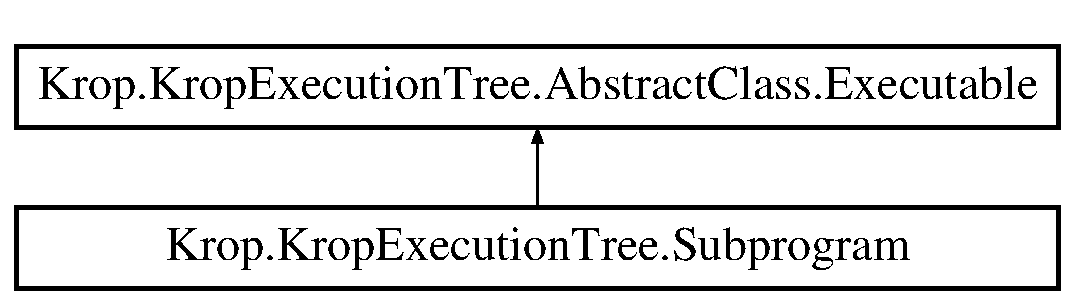
\includegraphics[height=2.000000cm]{class_krop_1_1_krop_execution_tree_1_1_subprogram}
\end{center}
\end{figure}
\subsection*{Public Member Functions}
\begin{DoxyCompactItemize}
\item 
\mbox{\hyperlink{class_krop_1_1_krop_execution_tree_1_1_subprogram_a200f90697de001a2fc317cd185db6b6b}{Subprogram}} (Node \+\_\+node\+Program)
\item 
\mbox{\hyperlink{class_krop_1_1_krop_execution_tree_1_1_subprogram_acfbfb331839d3687a7c417303ce3ea3d}{Subprogram}} (Node \+\_\+node\+Program, \mbox{\hyperlink{class_krop_1_1_krop_execution_tree_1_1_subprogram}{Subprogram}} \+\_\+subprogram\+Subprogram)
\item 
void \mbox{\hyperlink{class_krop_1_1_krop_execution_tree_1_1_subprogram_ae31602f28300c7cf092ac127b537a9df}{Add\+Instruction}} (\mbox{\hyperlink{class_krop_1_1_krop_execution_tree_1_1_abstract_class_1_1_executable}{Executable}} \+\_\+instruction)
\begin{DoxyCompactList}\small\item\em Add an executable object at the end of the subprogram \end{DoxyCompactList}\item 
override bool \mbox{\hyperlink{class_krop_1_1_krop_execution_tree_1_1_subprogram_ae33466ddf0761f860c5817a4263efd29}{Execute}} ()
\end{DoxyCompactItemize}
\subsection*{Static Public Member Functions}
\begin{DoxyCompactItemize}
\item 
static \mbox{\hyperlink{class_krop_1_1_krop_execution_tree_1_1_abstract_class_1_1_measurable}{Measurable}}$<$ Boolean $>$ \mbox{\hyperlink{class_krop_1_1_krop_execution_tree_1_1_subprogram_a3626c09fb9bf11430e8541e2c9740d81}{Set\+Cond}} (Node \+\_\+node\+Condition\+Statement, \mbox{\hyperlink{class_krop_1_1_krop_execution_tree_1_1_subprogram}{Subprogram}} \+\_\+parent\+Subprogram)
\begin{DoxyCompactList}\small\item\em Determine the condition type and create it \end{DoxyCompactList}\item 
static bool \mbox{\hyperlink{class_krop_1_1_krop_execution_tree_1_1_subprogram_af4e885168e0d7bbde2cf26f9f98c7af4}{Var\+Exists}} (string \+\_\+var\+Name, \mbox{\hyperlink{class_krop_1_1_krop_execution_tree_1_1_subprogram}{Subprogram}} \+\_\+parent\+Subprogram)
\begin{DoxyCompactList}\small\item\em Check if the variable already exists \end{DoxyCompactList}\item 
static string \mbox{\hyperlink{class_krop_1_1_krop_execution_tree_1_1_subprogram_abd8a129fb5f66a36c676c766561ffdea}{Var\+To\+String}} (string \+\_\+var\+Name, \mbox{\hyperlink{class_krop_1_1_krop_execution_tree_1_1_subprogram}{Subprogram}} \+\_\+parent\+Subprogram)
\begin{DoxyCompactList}\small\item\em Return the variable string \end{DoxyCompactList}\item 
static int \mbox{\hyperlink{class_krop_1_1_krop_execution_tree_1_1_subprogram_a3f33742aea9a7150f0dda2a17e84cf08}{Get\+Int\+Var\+Value}} (string \+\_\+var\+Name, \mbox{\hyperlink{class_krop_1_1_krop_execution_tree_1_1_subprogram}{Subprogram}} \+\_\+parent\+Subprogram)
\begin{DoxyCompactList}\small\item\em Return the value of an Int variable \end{DoxyCompactList}\item 
static \mbox{\hyperlink{interface_krop_1_1_krop_execution_tree_1_1_interface_1_1_i_variable}{I\+Variable}} \mbox{\hyperlink{class_krop_1_1_krop_execution_tree_1_1_subprogram_a51c0e1153e77771a566d7b6a96d0f26e}{Get\+Var}} (string \+\_\+var\+Name, \mbox{\hyperlink{class_krop_1_1_krop_execution_tree_1_1_subprogram}{Subprogram}} \+\_\+parent\+Subprogram)
\begin{DoxyCompactList}\small\item\em Return the variable \end{DoxyCompactList}\end{DoxyCompactItemize}
\subsection*{Public Attributes}
\begin{DoxyCompactItemize}
\item 
\mbox{\hyperlink{class_krop_1_1_krop_execution_tree_1_1_subprogram}{Subprogram}} \mbox{\hyperlink{class_krop_1_1_krop_execution_tree_1_1_subprogram_a8c7a1466aa0fa810acf3608419dae5d7}{Parent\+Subprogram}}
\item 
List$<$ \mbox{\hyperlink{interface_krop_1_1_krop_execution_tree_1_1_interface_1_1_i_variable}{I\+Variable}} $>$ \mbox{\hyperlink{class_krop_1_1_krop_execution_tree_1_1_subprogram_a22b8af148b8bf0bef634a3efb1290a94}{List\+Var}}
\end{DoxyCompactItemize}


\subsection{Detailed Description}
A \mbox{\hyperlink{class_krop_1_1_krop_execution_tree_1_1_subprogram}{Subprogram}} is a sequence of executable object (which can be subprograms!) 



\subsection{Constructor \& Destructor Documentation}
\mbox{\Hypertarget{class_krop_1_1_krop_execution_tree_1_1_subprogram_a200f90697de001a2fc317cd185db6b6b}\label{class_krop_1_1_krop_execution_tree_1_1_subprogram_a200f90697de001a2fc317cd185db6b6b}} 
\index{Krop\+::\+Krop\+Execution\+Tree\+::\+Subprogram@{Krop\+::\+Krop\+Execution\+Tree\+::\+Subprogram}!Subprogram@{Subprogram}}
\index{Subprogram@{Subprogram}!Krop\+::\+Krop\+Execution\+Tree\+::\+Subprogram@{Krop\+::\+Krop\+Execution\+Tree\+::\+Subprogram}}
\subsubsection{\texorpdfstring{Subprogram()}{Subprogram()}\hspace{0.1cm}{\footnotesize\ttfamily [1/2]}}
{\footnotesize\ttfamily Krop.\+Krop\+Execution\+Tree.\+Subprogram.\+Subprogram (\begin{DoxyParamCaption}\item[{Node}]{\+\_\+node\+Program }\end{DoxyParamCaption})}

\mbox{\Hypertarget{class_krop_1_1_krop_execution_tree_1_1_subprogram_acfbfb331839d3687a7c417303ce3ea3d}\label{class_krop_1_1_krop_execution_tree_1_1_subprogram_acfbfb331839d3687a7c417303ce3ea3d}} 
\index{Krop\+::\+Krop\+Execution\+Tree\+::\+Subprogram@{Krop\+::\+Krop\+Execution\+Tree\+::\+Subprogram}!Subprogram@{Subprogram}}
\index{Subprogram@{Subprogram}!Krop\+::\+Krop\+Execution\+Tree\+::\+Subprogram@{Krop\+::\+Krop\+Execution\+Tree\+::\+Subprogram}}
\subsubsection{\texorpdfstring{Subprogram()}{Subprogram()}\hspace{0.1cm}{\footnotesize\ttfamily [2/2]}}
{\footnotesize\ttfamily Krop.\+Krop\+Execution\+Tree.\+Subprogram.\+Subprogram (\begin{DoxyParamCaption}\item[{Node}]{\+\_\+node\+Program,  }\item[{\mbox{\hyperlink{class_krop_1_1_krop_execution_tree_1_1_subprogram}{Subprogram}}}]{\+\_\+subprogram\+Subprogram }\end{DoxyParamCaption})}



\subsection{Member Function Documentation}
\mbox{\Hypertarget{class_krop_1_1_krop_execution_tree_1_1_subprogram_ae31602f28300c7cf092ac127b537a9df}\label{class_krop_1_1_krop_execution_tree_1_1_subprogram_ae31602f28300c7cf092ac127b537a9df}} 
\index{Krop\+::\+Krop\+Execution\+Tree\+::\+Subprogram@{Krop\+::\+Krop\+Execution\+Tree\+::\+Subprogram}!Add\+Instruction@{Add\+Instruction}}
\index{Add\+Instruction@{Add\+Instruction}!Krop\+::\+Krop\+Execution\+Tree\+::\+Subprogram@{Krop\+::\+Krop\+Execution\+Tree\+::\+Subprogram}}
\subsubsection{\texorpdfstring{Add\+Instruction()}{AddInstruction()}}
{\footnotesize\ttfamily void Krop.\+Krop\+Execution\+Tree.\+Subprogram.\+Add\+Instruction (\begin{DoxyParamCaption}\item[{\mbox{\hyperlink{class_krop_1_1_krop_execution_tree_1_1_abstract_class_1_1_executable}{Executable}}}]{\+\_\+instruction }\end{DoxyParamCaption})}



Add an executable object at the end of the subprogram 

\mbox{\Hypertarget{class_krop_1_1_krop_execution_tree_1_1_subprogram_ae33466ddf0761f860c5817a4263efd29}\label{class_krop_1_1_krop_execution_tree_1_1_subprogram_ae33466ddf0761f860c5817a4263efd29}} 
\index{Krop\+::\+Krop\+Execution\+Tree\+::\+Subprogram@{Krop\+::\+Krop\+Execution\+Tree\+::\+Subprogram}!Execute@{Execute}}
\index{Execute@{Execute}!Krop\+::\+Krop\+Execution\+Tree\+::\+Subprogram@{Krop\+::\+Krop\+Execution\+Tree\+::\+Subprogram}}
\subsubsection{\texorpdfstring{Execute()}{Execute()}}
{\footnotesize\ttfamily override bool Krop.\+Krop\+Execution\+Tree.\+Subprogram.\+Execute (\begin{DoxyParamCaption}{ }\end{DoxyParamCaption})\hspace{0.3cm}{\ttfamily [virtual]}}



Implements \mbox{\hyperlink{class_krop_1_1_krop_execution_tree_1_1_abstract_class_1_1_executable_ac32692ce44b5f938a90111ee27e7b684}{Krop.\+Krop\+Execution\+Tree.\+Abstract\+Class.\+Executable}}.

\mbox{\Hypertarget{class_krop_1_1_krop_execution_tree_1_1_subprogram_a3f33742aea9a7150f0dda2a17e84cf08}\label{class_krop_1_1_krop_execution_tree_1_1_subprogram_a3f33742aea9a7150f0dda2a17e84cf08}} 
\index{Krop\+::\+Krop\+Execution\+Tree\+::\+Subprogram@{Krop\+::\+Krop\+Execution\+Tree\+::\+Subprogram}!Get\+Int\+Var\+Value@{Get\+Int\+Var\+Value}}
\index{Get\+Int\+Var\+Value@{Get\+Int\+Var\+Value}!Krop\+::\+Krop\+Execution\+Tree\+::\+Subprogram@{Krop\+::\+Krop\+Execution\+Tree\+::\+Subprogram}}
\subsubsection{\texorpdfstring{Get\+Int\+Var\+Value()}{GetIntVarValue()}}
{\footnotesize\ttfamily static int Krop.\+Krop\+Execution\+Tree.\+Subprogram.\+Get\+Int\+Var\+Value (\begin{DoxyParamCaption}\item[{string}]{\+\_\+var\+Name,  }\item[{\mbox{\hyperlink{class_krop_1_1_krop_execution_tree_1_1_subprogram}{Subprogram}}}]{\+\_\+parent\+Subprogram }\end{DoxyParamCaption})\hspace{0.3cm}{\ttfamily [static]}}



Return the value of an Int variable 


\begin{DoxyParams}{Parameters}
{\em \+\_\+var\+Name} & \mbox{\hyperlink{namespace_krop_1_1_krop_execution_tree_1_1_variable}{Variable}} Name\\
\hline
{\em \+\_\+parent\+Subprogram} & Parent \mbox{\hyperlink{class_krop_1_1_krop_execution_tree_1_1_subprogram}{Subprogram}}\\
\hline
\end{DoxyParams}
\begin{DoxyReturn}{Returns}
Int variable value
\end{DoxyReturn}
\mbox{\Hypertarget{class_krop_1_1_krop_execution_tree_1_1_subprogram_a51c0e1153e77771a566d7b6a96d0f26e}\label{class_krop_1_1_krop_execution_tree_1_1_subprogram_a51c0e1153e77771a566d7b6a96d0f26e}} 
\index{Krop\+::\+Krop\+Execution\+Tree\+::\+Subprogram@{Krop\+::\+Krop\+Execution\+Tree\+::\+Subprogram}!Get\+Var@{Get\+Var}}
\index{Get\+Var@{Get\+Var}!Krop\+::\+Krop\+Execution\+Tree\+::\+Subprogram@{Krop\+::\+Krop\+Execution\+Tree\+::\+Subprogram}}
\subsubsection{\texorpdfstring{Get\+Var()}{GetVar()}}
{\footnotesize\ttfamily static \mbox{\hyperlink{interface_krop_1_1_krop_execution_tree_1_1_interface_1_1_i_variable}{I\+Variable}} Krop.\+Krop\+Execution\+Tree.\+Subprogram.\+Get\+Var (\begin{DoxyParamCaption}\item[{string}]{\+\_\+var\+Name,  }\item[{\mbox{\hyperlink{class_krop_1_1_krop_execution_tree_1_1_subprogram}{Subprogram}}}]{\+\_\+parent\+Subprogram }\end{DoxyParamCaption})\hspace{0.3cm}{\ttfamily [static]}}



Return the variable 


\begin{DoxyParams}{Parameters}
{\em \+\_\+var\+Name} & \mbox{\hyperlink{namespace_krop_1_1_krop_execution_tree_1_1_variable}{Variable}} Name\\
\hline
{\em \+\_\+parent\+Subprogram} & Parent \mbox{\hyperlink{class_krop_1_1_krop_execution_tree_1_1_subprogram}{Subprogram}}\\
\hline
\end{DoxyParams}
\begin{DoxyReturn}{Returns}
\mbox{\hyperlink{namespace_krop_1_1_krop_execution_tree_1_1_variable}{Variable}}
\end{DoxyReturn}
\mbox{\Hypertarget{class_krop_1_1_krop_execution_tree_1_1_subprogram_a3626c09fb9bf11430e8541e2c9740d81}\label{class_krop_1_1_krop_execution_tree_1_1_subprogram_a3626c09fb9bf11430e8541e2c9740d81}} 
\index{Krop\+::\+Krop\+Execution\+Tree\+::\+Subprogram@{Krop\+::\+Krop\+Execution\+Tree\+::\+Subprogram}!Set\+Cond@{Set\+Cond}}
\index{Set\+Cond@{Set\+Cond}!Krop\+::\+Krop\+Execution\+Tree\+::\+Subprogram@{Krop\+::\+Krop\+Execution\+Tree\+::\+Subprogram}}
\subsubsection{\texorpdfstring{Set\+Cond()}{SetCond()}}
{\footnotesize\ttfamily static \mbox{\hyperlink{class_krop_1_1_krop_execution_tree_1_1_abstract_class_1_1_measurable}{Measurable}}$<$Boolean$>$ Krop.\+Krop\+Execution\+Tree.\+Subprogram.\+Set\+Cond (\begin{DoxyParamCaption}\item[{Node}]{\+\_\+node\+Condition\+Statement,  }\item[{\mbox{\hyperlink{class_krop_1_1_krop_execution_tree_1_1_subprogram}{Subprogram}}}]{\+\_\+parent\+Subprogram }\end{DoxyParamCaption})\hspace{0.3cm}{\ttfamily [static]}}



Determine the condition type and create it 


\begin{DoxyParams}{Parameters}
{\em \+\_\+node\+Condition\+Statement} & Node containing the \mbox{\hyperlink{namespace_krop_1_1_krop_execution_tree_1_1_condition}{Condition}}\\
\hline
\end{DoxyParams}
\begin{DoxyReturn}{Returns}

\end{DoxyReturn}
\mbox{\Hypertarget{class_krop_1_1_krop_execution_tree_1_1_subprogram_af4e885168e0d7bbde2cf26f9f98c7af4}\label{class_krop_1_1_krop_execution_tree_1_1_subprogram_af4e885168e0d7bbde2cf26f9f98c7af4}} 
\index{Krop\+::\+Krop\+Execution\+Tree\+::\+Subprogram@{Krop\+::\+Krop\+Execution\+Tree\+::\+Subprogram}!Var\+Exists@{Var\+Exists}}
\index{Var\+Exists@{Var\+Exists}!Krop\+::\+Krop\+Execution\+Tree\+::\+Subprogram@{Krop\+::\+Krop\+Execution\+Tree\+::\+Subprogram}}
\subsubsection{\texorpdfstring{Var\+Exists()}{VarExists()}}
{\footnotesize\ttfamily static bool Krop.\+Krop\+Execution\+Tree.\+Subprogram.\+Var\+Exists (\begin{DoxyParamCaption}\item[{string}]{\+\_\+var\+Name,  }\item[{\mbox{\hyperlink{class_krop_1_1_krop_execution_tree_1_1_subprogram}{Subprogram}}}]{\+\_\+parent\+Subprogram }\end{DoxyParamCaption})\hspace{0.3cm}{\ttfamily [static]}}



Check if the variable already exists 


\begin{DoxyParams}{Parameters}
{\em \+\_\+var\+Name} & \mbox{\hyperlink{namespace_krop_1_1_krop_execution_tree_1_1_variable}{Variable}} Name\\
\hline
{\em \+\_\+parent\+Subprogram} & Parent \mbox{\hyperlink{class_krop_1_1_krop_execution_tree_1_1_subprogram}{Subprogram}}\\
\hline
\end{DoxyParams}
\begin{DoxyReturn}{Returns}
Result
\end{DoxyReturn}
\mbox{\Hypertarget{class_krop_1_1_krop_execution_tree_1_1_subprogram_abd8a129fb5f66a36c676c766561ffdea}\label{class_krop_1_1_krop_execution_tree_1_1_subprogram_abd8a129fb5f66a36c676c766561ffdea}} 
\index{Krop\+::\+Krop\+Execution\+Tree\+::\+Subprogram@{Krop\+::\+Krop\+Execution\+Tree\+::\+Subprogram}!Var\+To\+String@{Var\+To\+String}}
\index{Var\+To\+String@{Var\+To\+String}!Krop\+::\+Krop\+Execution\+Tree\+::\+Subprogram@{Krop\+::\+Krop\+Execution\+Tree\+::\+Subprogram}}
\subsubsection{\texorpdfstring{Var\+To\+String()}{VarToString()}}
{\footnotesize\ttfamily static string Krop.\+Krop\+Execution\+Tree.\+Subprogram.\+Var\+To\+String (\begin{DoxyParamCaption}\item[{string}]{\+\_\+var\+Name,  }\item[{\mbox{\hyperlink{class_krop_1_1_krop_execution_tree_1_1_subprogram}{Subprogram}}}]{\+\_\+parent\+Subprogram }\end{DoxyParamCaption})\hspace{0.3cm}{\ttfamily [static]}}



Return the variable string 


\begin{DoxyParams}{Parameters}
{\em \+\_\+var\+Name} & \mbox{\hyperlink{namespace_krop_1_1_krop_execution_tree_1_1_variable}{Variable}} Name\\
\hline
{\em \+\_\+parent\+Subprogram} & Parent \mbox{\hyperlink{class_krop_1_1_krop_execution_tree_1_1_subprogram}{Subprogram}}\\
\hline
\end{DoxyParams}
\begin{DoxyReturn}{Returns}
\mbox{\hyperlink{namespace_krop_1_1_krop_execution_tree_1_1_variable}{Variable}} string
\end{DoxyReturn}


\subsection{Member Data Documentation}
\mbox{\Hypertarget{class_krop_1_1_krop_execution_tree_1_1_subprogram_a22b8af148b8bf0bef634a3efb1290a94}\label{class_krop_1_1_krop_execution_tree_1_1_subprogram_a22b8af148b8bf0bef634a3efb1290a94}} 
\index{Krop\+::\+Krop\+Execution\+Tree\+::\+Subprogram@{Krop\+::\+Krop\+Execution\+Tree\+::\+Subprogram}!List\+Var@{List\+Var}}
\index{List\+Var@{List\+Var}!Krop\+::\+Krop\+Execution\+Tree\+::\+Subprogram@{Krop\+::\+Krop\+Execution\+Tree\+::\+Subprogram}}
\subsubsection{\texorpdfstring{List\+Var}{ListVar}}
{\footnotesize\ttfamily List$<$\mbox{\hyperlink{interface_krop_1_1_krop_execution_tree_1_1_interface_1_1_i_variable}{I\+Variable}}$>$ Krop.\+Krop\+Execution\+Tree.\+Subprogram.\+List\+Var}

\mbox{\Hypertarget{class_krop_1_1_krop_execution_tree_1_1_subprogram_a8c7a1466aa0fa810acf3608419dae5d7}\label{class_krop_1_1_krop_execution_tree_1_1_subprogram_a8c7a1466aa0fa810acf3608419dae5d7}} 
\index{Krop\+::\+Krop\+Execution\+Tree\+::\+Subprogram@{Krop\+::\+Krop\+Execution\+Tree\+::\+Subprogram}!Parent\+Subprogram@{Parent\+Subprogram}}
\index{Parent\+Subprogram@{Parent\+Subprogram}!Krop\+::\+Krop\+Execution\+Tree\+::\+Subprogram@{Krop\+::\+Krop\+Execution\+Tree\+::\+Subprogram}}
\subsubsection{\texorpdfstring{Parent\+Subprogram}{ParentSubprogram}}
{\footnotesize\ttfamily \mbox{\hyperlink{class_krop_1_1_krop_execution_tree_1_1_subprogram}{Subprogram}} Krop.\+Krop\+Execution\+Tree.\+Subprogram.\+Parent\+Subprogram}



The documentation for this class was generated from the following file\+:\begin{DoxyCompactItemize}
\item 
C\+:/\+Users/\+Stuart.\+G\+U\+E\+I\+S\+S\+A\+Z/\+Documents/\+Git\+Hub/\+Krop/\+Code/\+Krop/\+Krop\+Execution\+Tree/\mbox{\hyperlink{_subprogram_8cs}{Subprogram.\+cs}}\end{DoxyCompactItemize}

\hypertarget{class_krop_1_1_krohonde_1_1_texture2_d}{}\section{Krop.\+Krohonde.\+Texture2D Class Reference}
\label{class_krop_1_1_krohonde_1_1_texture2_d}\index{Krop.\+Krohonde.\+Texture2D@{Krop.\+Krohonde.\+Texture2D}}
\subsection*{Public Member Functions}
\begin{DoxyCompactItemize}
\item 
\mbox{\hyperlink{class_krop_1_1_krohonde_1_1_texture2_d_a9558de84975b10d522dff486aca06343}{Texture2D}} (int id, int width, int height)
\end{DoxyCompactItemize}
\subsection*{Properties}
\begin{DoxyCompactItemize}
\item 
int \mbox{\hyperlink{class_krop_1_1_krohonde_1_1_texture2_d_aa5b329a7dc50ebb6193cc0d63b205631}{ID}}\hspace{0.3cm}{\ttfamily  \mbox{[}get\mbox{]}}
\item 
int \mbox{\hyperlink{class_krop_1_1_krohonde_1_1_texture2_d_adac0dafaf47b7ed77eb6fc9bf43972d6}{Width}}\hspace{0.3cm}{\ttfamily  \mbox{[}get\mbox{]}}
\item 
int \mbox{\hyperlink{class_krop_1_1_krohonde_1_1_texture2_d_a1ee6a5a7735251a27cb865ab805c8571}{Height}}\hspace{0.3cm}{\ttfamily  \mbox{[}get\mbox{]}}
\end{DoxyCompactItemize}


\subsection{Constructor \& Destructor Documentation}
\mbox{\Hypertarget{class_krop_1_1_krohonde_1_1_texture2_d_a9558de84975b10d522dff486aca06343}\label{class_krop_1_1_krohonde_1_1_texture2_d_a9558de84975b10d522dff486aca06343}} 
\index{Krop\+::\+Krohonde\+::\+Texture2D@{Krop\+::\+Krohonde\+::\+Texture2D}!Texture2D@{Texture2D}}
\index{Texture2D@{Texture2D}!Krop\+::\+Krohonde\+::\+Texture2D@{Krop\+::\+Krohonde\+::\+Texture2D}}
\subsubsection{\texorpdfstring{Texture2\+D()}{Texture2D()}}
{\footnotesize\ttfamily Krop.\+Krohonde.\+Texture2\+D.\+Texture2D (\begin{DoxyParamCaption}\item[{int}]{id,  }\item[{int}]{width,  }\item[{int}]{height }\end{DoxyParamCaption})}



\subsection{Property Documentation}
\mbox{\Hypertarget{class_krop_1_1_krohonde_1_1_texture2_d_a1ee6a5a7735251a27cb865ab805c8571}\label{class_krop_1_1_krohonde_1_1_texture2_d_a1ee6a5a7735251a27cb865ab805c8571}} 
\index{Krop\+::\+Krohonde\+::\+Texture2D@{Krop\+::\+Krohonde\+::\+Texture2D}!Height@{Height}}
\index{Height@{Height}!Krop\+::\+Krohonde\+::\+Texture2D@{Krop\+::\+Krohonde\+::\+Texture2D}}
\subsubsection{\texorpdfstring{Height}{Height}}
{\footnotesize\ttfamily int Krop.\+Krohonde.\+Texture2\+D.\+Height\hspace{0.3cm}{\ttfamily [get]}}

\mbox{\Hypertarget{class_krop_1_1_krohonde_1_1_texture2_d_aa5b329a7dc50ebb6193cc0d63b205631}\label{class_krop_1_1_krohonde_1_1_texture2_d_aa5b329a7dc50ebb6193cc0d63b205631}} 
\index{Krop\+::\+Krohonde\+::\+Texture2D@{Krop\+::\+Krohonde\+::\+Texture2D}!ID@{ID}}
\index{ID@{ID}!Krop\+::\+Krohonde\+::\+Texture2D@{Krop\+::\+Krohonde\+::\+Texture2D}}
\subsubsection{\texorpdfstring{ID}{ID}}
{\footnotesize\ttfamily int Krop.\+Krohonde.\+Texture2\+D.\+ID\hspace{0.3cm}{\ttfamily [get]}}

\mbox{\Hypertarget{class_krop_1_1_krohonde_1_1_texture2_d_adac0dafaf47b7ed77eb6fc9bf43972d6}\label{class_krop_1_1_krohonde_1_1_texture2_d_adac0dafaf47b7ed77eb6fc9bf43972d6}} 
\index{Krop\+::\+Krohonde\+::\+Texture2D@{Krop\+::\+Krohonde\+::\+Texture2D}!Width@{Width}}
\index{Width@{Width}!Krop\+::\+Krohonde\+::\+Texture2D@{Krop\+::\+Krohonde\+::\+Texture2D}}
\subsubsection{\texorpdfstring{Width}{Width}}
{\footnotesize\ttfamily int Krop.\+Krohonde.\+Texture2\+D.\+Width\hspace{0.3cm}{\ttfamily [get]}}



The documentation for this class was generated from the following file\+:\begin{DoxyCompactItemize}
\item 
C\+:/\+Users/\+Stuart.\+G\+U\+E\+I\+S\+S\+A\+Z/\+Documents/\+Git\+Hub/\+Krop/\+Code/\+Krop/\+Krohonde/\mbox{\hyperlink{_texture2_d_8cs}{Texture2\+D.\+cs}}\end{DoxyCompactItemize}

\hypertarget{class_krop_1_1_krop_execution_tree_1_1_abstract_class_1_1_variable}{}\section{Krop.\+Krop\+Execution\+Tree.\+Abstract\+Class.\+Variable$<$ T $>$ Class Template Reference}
\label{class_krop_1_1_krop_execution_tree_1_1_abstract_class_1_1_variable}\index{Krop.\+Krop\+Execution\+Tree.\+Abstract\+Class.\+Variable$<$ T $>$@{Krop.\+Krop\+Execution\+Tree.\+Abstract\+Class.\+Variable$<$ T $>$}}


\mbox{\hyperlink{class_krop_1_1_krop_execution_tree_1_1_abstract_class_1_1_variable}{Variable}} objects The variable is of type T  


Inheritance diagram for Krop.\+Krop\+Execution\+Tree.\+Abstract\+Class.\+Variable$<$ T $>$\+:\begin{figure}[H]
\begin{center}
\leavevmode
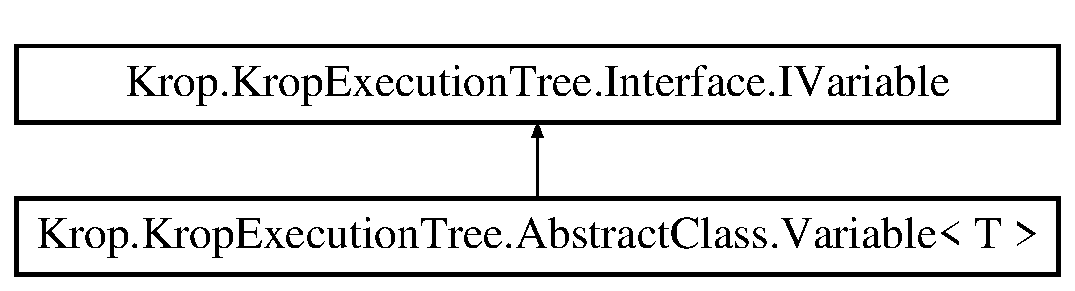
\includegraphics[height=2.000000cm]{class_krop_1_1_krop_execution_tree_1_1_abstract_class_1_1_variable}
\end{center}
\end{figure}
\subsection*{Public Member Functions}
\begin{DoxyCompactItemize}
\item 
abstract string \mbox{\hyperlink{class_krop_1_1_krop_execution_tree_1_1_abstract_class_1_1_variable_a987550c24ebd0ceb01aec0b6edf51dfb}{Get\+Name}} ()
\item 
abstract void \mbox{\hyperlink{class_krop_1_1_krop_execution_tree_1_1_abstract_class_1_1_variable_ac2022740855edfe2c1fdcea60d877fa4}{Set\+Value}} (T \+\_\+value)
\item 
abstract T \mbox{\hyperlink{class_krop_1_1_krop_execution_tree_1_1_abstract_class_1_1_variable_a9d77d99b187893c15c5847ffa6fe0daf}{Get\+Value}} ()
\item 
abstract override string \mbox{\hyperlink{class_krop_1_1_krop_execution_tree_1_1_abstract_class_1_1_variable_ae78ccbb029efb966e1edff0ae101f367}{To\+String}} ()
\end{DoxyCompactItemize}


\subsection{Detailed Description}
\mbox{\hyperlink{class_krop_1_1_krop_execution_tree_1_1_abstract_class_1_1_variable}{Variable}} objects The variable is of type T 


\begin{DoxyTemplParams}{Template Parameters}
{\em T} & \\
\hline
\end{DoxyTemplParams}


\subsection{Member Function Documentation}
\mbox{\Hypertarget{class_krop_1_1_krop_execution_tree_1_1_abstract_class_1_1_variable_a987550c24ebd0ceb01aec0b6edf51dfb}\label{class_krop_1_1_krop_execution_tree_1_1_abstract_class_1_1_variable_a987550c24ebd0ceb01aec0b6edf51dfb}} 
\index{Krop\+::\+Krop\+Execution\+Tree\+::\+Abstract\+Class\+::\+Variable@{Krop\+::\+Krop\+Execution\+Tree\+::\+Abstract\+Class\+::\+Variable}!Get\+Name@{Get\+Name}}
\index{Get\+Name@{Get\+Name}!Krop\+::\+Krop\+Execution\+Tree\+::\+Abstract\+Class\+::\+Variable@{Krop\+::\+Krop\+Execution\+Tree\+::\+Abstract\+Class\+::\+Variable}}
\subsubsection{\texorpdfstring{Get\+Name()}{GetName()}}
{\footnotesize\ttfamily abstract string \mbox{\hyperlink{class_krop_1_1_krop_execution_tree_1_1_abstract_class_1_1_variable}{Krop.\+Krop\+Execution\+Tree.\+Abstract\+Class.\+Variable}}$<$ T $>$.Get\+Name (\begin{DoxyParamCaption}{ }\end{DoxyParamCaption})\hspace{0.3cm}{\ttfamily [pure virtual]}}



Implements \mbox{\hyperlink{interface_krop_1_1_krop_execution_tree_1_1_interface_1_1_i_variable_a0a1ca374f3af72c44d0754c00e8c26d3}{Krop.\+Krop\+Execution\+Tree.\+Interface.\+I\+Variable}}.



Implemented in \mbox{\hyperlink{class_krop_1_1_krop_execution_tree_1_1_variable_1_1_int_var_ae48d754976bd6ed849a048ae209a689a}{Krop.\+Krop\+Execution\+Tree.\+Variable.\+Int\+Var}}.

\mbox{\Hypertarget{class_krop_1_1_krop_execution_tree_1_1_abstract_class_1_1_variable_a9d77d99b187893c15c5847ffa6fe0daf}\label{class_krop_1_1_krop_execution_tree_1_1_abstract_class_1_1_variable_a9d77d99b187893c15c5847ffa6fe0daf}} 
\index{Krop\+::\+Krop\+Execution\+Tree\+::\+Abstract\+Class\+::\+Variable@{Krop\+::\+Krop\+Execution\+Tree\+::\+Abstract\+Class\+::\+Variable}!Get\+Value@{Get\+Value}}
\index{Get\+Value@{Get\+Value}!Krop\+::\+Krop\+Execution\+Tree\+::\+Abstract\+Class\+::\+Variable@{Krop\+::\+Krop\+Execution\+Tree\+::\+Abstract\+Class\+::\+Variable}}
\subsubsection{\texorpdfstring{Get\+Value()}{GetValue()}}
{\footnotesize\ttfamily abstract T \mbox{\hyperlink{class_krop_1_1_krop_execution_tree_1_1_abstract_class_1_1_variable}{Krop.\+Krop\+Execution\+Tree.\+Abstract\+Class.\+Variable}}$<$ T $>$.Get\+Value (\begin{DoxyParamCaption}{ }\end{DoxyParamCaption})\hspace{0.3cm}{\ttfamily [pure virtual]}}



Implemented in \mbox{\hyperlink{class_krop_1_1_krop_execution_tree_1_1_variable_1_1_int_var_a286e20f12bf8a03b9586596253a97144}{Krop.\+Krop\+Execution\+Tree.\+Variable.\+Int\+Var}}.

\mbox{\Hypertarget{class_krop_1_1_krop_execution_tree_1_1_abstract_class_1_1_variable_ac2022740855edfe2c1fdcea60d877fa4}\label{class_krop_1_1_krop_execution_tree_1_1_abstract_class_1_1_variable_ac2022740855edfe2c1fdcea60d877fa4}} 
\index{Krop\+::\+Krop\+Execution\+Tree\+::\+Abstract\+Class\+::\+Variable@{Krop\+::\+Krop\+Execution\+Tree\+::\+Abstract\+Class\+::\+Variable}!Set\+Value@{Set\+Value}}
\index{Set\+Value@{Set\+Value}!Krop\+::\+Krop\+Execution\+Tree\+::\+Abstract\+Class\+::\+Variable@{Krop\+::\+Krop\+Execution\+Tree\+::\+Abstract\+Class\+::\+Variable}}
\subsubsection{\texorpdfstring{Set\+Value()}{SetValue()}}
{\footnotesize\ttfamily abstract void \mbox{\hyperlink{class_krop_1_1_krop_execution_tree_1_1_abstract_class_1_1_variable}{Krop.\+Krop\+Execution\+Tree.\+Abstract\+Class.\+Variable}}$<$ T $>$.Set\+Value (\begin{DoxyParamCaption}\item[{T}]{\+\_\+value }\end{DoxyParamCaption})\hspace{0.3cm}{\ttfamily [pure virtual]}}

\mbox{\Hypertarget{class_krop_1_1_krop_execution_tree_1_1_abstract_class_1_1_variable_ae78ccbb029efb966e1edff0ae101f367}\label{class_krop_1_1_krop_execution_tree_1_1_abstract_class_1_1_variable_ae78ccbb029efb966e1edff0ae101f367}} 
\index{Krop\+::\+Krop\+Execution\+Tree\+::\+Abstract\+Class\+::\+Variable@{Krop\+::\+Krop\+Execution\+Tree\+::\+Abstract\+Class\+::\+Variable}!To\+String@{To\+String}}
\index{To\+String@{To\+String}!Krop\+::\+Krop\+Execution\+Tree\+::\+Abstract\+Class\+::\+Variable@{Krop\+::\+Krop\+Execution\+Tree\+::\+Abstract\+Class\+::\+Variable}}
\subsubsection{\texorpdfstring{To\+String()}{ToString()}}
{\footnotesize\ttfamily abstract override string \mbox{\hyperlink{class_krop_1_1_krop_execution_tree_1_1_abstract_class_1_1_variable}{Krop.\+Krop\+Execution\+Tree.\+Abstract\+Class.\+Variable}}$<$ T $>$.To\+String (\begin{DoxyParamCaption}{ }\end{DoxyParamCaption})\hspace{0.3cm}{\ttfamily [pure virtual]}}



Implements \mbox{\hyperlink{interface_krop_1_1_krop_execution_tree_1_1_interface_1_1_i_variable_a4d3f36256ae24e2550ee0a16d3142822}{Krop.\+Krop\+Execution\+Tree.\+Interface.\+I\+Variable}}.



Implemented in \mbox{\hyperlink{class_krop_1_1_krop_execution_tree_1_1_variable_1_1_int_var_acfe213da1e8d6fb0590872d3e7f9195b}{Krop.\+Krop\+Execution\+Tree.\+Variable.\+Int\+Var}}.



The documentation for this class was generated from the following file\+:\begin{DoxyCompactItemize}
\item 
C\+:/\+Users/\+Stuart.\+G\+U\+E\+I\+S\+S\+A\+Z/\+Documents/\+Git\+Hub/\+Krop/\+Code/\+Krop/\+Krop\+Execution\+Tree/\+Abstract\+Class/\mbox{\hyperlink{_variable_8cs}{Variable.\+cs}}\end{DoxyCompactItemize}

\chapter{File Documentation}
\hypertarget{_form_control_window_8cs}{}\section{C\+:/\+Users/\+Stuart.G\+U\+E\+I\+S\+S\+A\+Z/\+Documents/\+Git\+Hub/\+Krop/\+Code/\+Krop/\+Control\+Window/\+Form\+Control\+Window.cs File Reference}
\label{_form_control_window_8cs}\index{C\+:/\+Users/\+Stuart.\+G\+U\+E\+I\+S\+S\+A\+Z/\+Documents/\+Git\+Hub/\+Krop/\+Code/\+Krop/\+Control\+Window/\+Form\+Control\+Window.\+cs@{C\+:/\+Users/\+Stuart.\+G\+U\+E\+I\+S\+S\+A\+Z/\+Documents/\+Git\+Hub/\+Krop/\+Code/\+Krop/\+Control\+Window/\+Form\+Control\+Window.\+cs}}
\subsection*{Classes}
\begin{DoxyCompactItemize}
\item 
class \mbox{\hyperlink{class_krop_1_1_control_window_1_1_form_control_window}{Krop.\+Control\+Window.\+Form\+Control\+Window}}
\end{DoxyCompactItemize}
\subsection*{Namespaces}
\begin{DoxyCompactItemize}
\item 
namespace \mbox{\hyperlink{namespace_krop_1_1_control_window}{Krop.\+Control\+Window}}
\end{DoxyCompactItemize}

\hypertarget{_form_control_window_8_designer_8cs}{}\section{C\+:/\+Users/\+Stuart.G\+U\+E\+I\+S\+S\+A\+Z/\+Documents/\+Git\+Hub/\+Krop/\+Code/\+Krop/\+Control\+Window/\+Form\+Control\+Window.Designer.\+cs File Reference}
\label{_form_control_window_8_designer_8cs}\index{C\+:/\+Users/\+Stuart.\+G\+U\+E\+I\+S\+S\+A\+Z/\+Documents/\+Git\+Hub/\+Krop/\+Code/\+Krop/\+Control\+Window/\+Form\+Control\+Window.\+Designer.\+cs@{C\+:/\+Users/\+Stuart.\+G\+U\+E\+I\+S\+S\+A\+Z/\+Documents/\+Git\+Hub/\+Krop/\+Code/\+Krop/\+Control\+Window/\+Form\+Control\+Window.\+Designer.\+cs}}
\subsection*{Classes}
\begin{DoxyCompactItemize}
\item 
class \mbox{\hyperlink{class_krop_1_1_control_window_1_1_form_control_window}{Krop.\+Control\+Window.\+Form\+Control\+Window}}
\end{DoxyCompactItemize}
\subsection*{Namespaces}
\begin{DoxyCompactItemize}
\item 
namespace \mbox{\hyperlink{namespace_krop_1_1_control_window}{Krop.\+Control\+Window}}
\end{DoxyCompactItemize}

\hypertarget{_ant_8cs}{}\section{C\+:/\+Users/\+Stuart.G\+U\+E\+I\+S\+S\+A\+Z/\+Documents/\+Git\+Hub/\+Krop/\+Code/\+Krop/\+Krohonde/\+Ant.cs File Reference}
\label{_ant_8cs}\index{C\+:/\+Users/\+Stuart.\+G\+U\+E\+I\+S\+S\+A\+Z/\+Documents/\+Git\+Hub/\+Krop/\+Code/\+Krop/\+Krohonde/\+Ant.\+cs@{C\+:/\+Users/\+Stuart.\+G\+U\+E\+I\+S\+S\+A\+Z/\+Documents/\+Git\+Hub/\+Krop/\+Code/\+Krop/\+Krohonde/\+Ant.\+cs}}
\subsection*{Classes}
\begin{DoxyCompactItemize}
\item 
class \mbox{\hyperlink{class_krop_1_1_krohonde_1_1_ant}{Krop.\+Krohonde.\+Ant}}
\begin{DoxyCompactList}\small\item\em Hold a \mbox{\hyperlink{class_krop_1_1_krohonde_1_1_ant}{Ant}} \end{DoxyCompactList}\end{DoxyCompactItemize}
\subsection*{Namespaces}
\begin{DoxyCompactItemize}
\item 
namespace \mbox{\hyperlink{namespace_krop_1_1_krohonde}{Krop.\+Krohonde}}
\end{DoxyCompactItemize}

\hypertarget{_content_pipe_8cs}{}\section{C\+:/\+Users/\+Stuart.G\+U\+E\+I\+S\+S\+A\+Z/\+Documents/\+Git\+Hub/\+Krop/\+Code/\+Krop/\+Krohonde/\+Content\+Pipe.cs File Reference}
\label{_content_pipe_8cs}\index{C\+:/\+Users/\+Stuart.\+G\+U\+E\+I\+S\+S\+A\+Z/\+Documents/\+Git\+Hub/\+Krop/\+Code/\+Krop/\+Krohonde/\+Content\+Pipe.\+cs@{C\+:/\+Users/\+Stuart.\+G\+U\+E\+I\+S\+S\+A\+Z/\+Documents/\+Git\+Hub/\+Krop/\+Code/\+Krop/\+Krohonde/\+Content\+Pipe.\+cs}}
\subsection*{Classes}
\begin{DoxyCompactItemize}
\item 
class \mbox{\hyperlink{class_krop_1_1_krohonde_1_1_content_pipe}{Krop.\+Krohonde.\+Content\+Pipe}}
\end{DoxyCompactItemize}
\subsection*{Namespaces}
\begin{DoxyCompactItemize}
\item 
namespace \mbox{\hyperlink{namespace_krop_1_1_krohonde}{Krop.\+Krohonde}}
\end{DoxyCompactItemize}

\hypertarget{_game_8cs}{}\section{C\+:/\+Users/\+Stuart.G\+U\+E\+I\+S\+S\+A\+Z/\+Documents/\+Git\+Hub/\+Krop/\+Code/\+Krop/\+Krohonde/\+Game.cs File Reference}
\label{_game_8cs}\index{C\+:/\+Users/\+Stuart.\+G\+U\+E\+I\+S\+S\+A\+Z/\+Documents/\+Git\+Hub/\+Krop/\+Code/\+Krop/\+Krohonde/\+Game.\+cs@{C\+:/\+Users/\+Stuart.\+G\+U\+E\+I\+S\+S\+A\+Z/\+Documents/\+Git\+Hub/\+Krop/\+Code/\+Krop/\+Krohonde/\+Game.\+cs}}
\subsection*{Classes}
\begin{DoxyCompactItemize}
\item 
class \mbox{\hyperlink{class_krop_1_1_krohonde_1_1_game}{Krop.\+Krohonde.\+Game}}
\begin{DoxyCompactList}\small\item\em Primary class of the project \end{DoxyCompactList}\end{DoxyCompactItemize}
\subsection*{Namespaces}
\begin{DoxyCompactItemize}
\item 
namespace \mbox{\hyperlink{namespace_krop_1_1_krohonde}{Krop.\+Krohonde}}
\end{DoxyCompactItemize}
\subsection*{Enumerations}
\begin{DoxyCompactItemize}
\item 
enum \mbox{\hyperlink{namespace_krop_1_1_krohonde_a846d88876d5263c1530b67322bacd896}{Krop.\+Krohonde.\+Direction}} \{ \newline
\mbox{\hyperlink{namespace_krop_1_1_krohonde_a846d88876d5263c1530b67322bacd896a601560b94fbb188919dd1d36c8ab70a4}{Krop.\+Krohonde.\+Direction.\+North}} = 0, 
\mbox{\hyperlink{namespace_krop_1_1_krohonde_a846d88876d5263c1530b67322bacd896a7254edb19370d28e3466c971d2f8a03e}{Krop.\+Krohonde.\+Direction.\+North\+East}} = 45, 
\mbox{\hyperlink{namespace_krop_1_1_krohonde_a846d88876d5263c1530b67322bacd896aa99dc62d017d04cf67266593f9c3761e}{Krop.\+Krohonde.\+Direction.\+East}} = 90, 
\mbox{\hyperlink{namespace_krop_1_1_krohonde_a846d88876d5263c1530b67322bacd896a865a51dff69223f0cf5ad630e5ada190}{Krop.\+Krohonde.\+Direction.\+South\+East}} = 135, 
\newline
\mbox{\hyperlink{namespace_krop_1_1_krohonde_a846d88876d5263c1530b67322bacd896a263d7b2cf53802c9ed127b718c0bf9fd}{Krop.\+Krohonde.\+Direction.\+South}} = 180, 
\mbox{\hyperlink{namespace_krop_1_1_krohonde_a846d88876d5263c1530b67322bacd896ae8eaf797b01fdb4246ed54904368b592}{Krop.\+Krohonde.\+Direction.\+South\+West}} = 225, 
\mbox{\hyperlink{namespace_krop_1_1_krohonde_a846d88876d5263c1530b67322bacd896abf495fc048d8d44b7f32536df5cf3930}{Krop.\+Krohonde.\+Direction.\+West}} = 270, 
\mbox{\hyperlink{namespace_krop_1_1_krohonde_a846d88876d5263c1530b67322bacd896a142cbe82227bdec147eff3a629dd366b}{Krop.\+Krohonde.\+Direction.\+North\+West}} = 315
 \}
\begin{DoxyCompactList}\small\item\em Enum of the 8 cardinal points \end{DoxyCompactList}\end{DoxyCompactItemize}

\hypertarget{_level_8cs}{}\section{C\+:/\+Users/\+Stuart.G\+U\+E\+I\+S\+S\+A\+Z/\+Documents/\+Git\+Hub/\+Krop/\+Code/\+Krop/\+Krohonde/\+Level.cs File Reference}
\label{_level_8cs}\index{C\+:/\+Users/\+Stuart.\+G\+U\+E\+I\+S\+S\+A\+Z/\+Documents/\+Git\+Hub/\+Krop/\+Code/\+Krop/\+Krohonde/\+Level.\+cs@{C\+:/\+Users/\+Stuart.\+G\+U\+E\+I\+S\+S\+A\+Z/\+Documents/\+Git\+Hub/\+Krop/\+Code/\+Krop/\+Krohonde/\+Level.\+cs}}
\subsection*{Classes}
\begin{DoxyCompactItemize}
\item 
struct \mbox{\hyperlink{struct_krop_1_1_krohonde_1_1_level}{Krop.\+Krohonde.\+Level}}
\item 
struct \mbox{\hyperlink{struct_krop_1_1_krohonde_1_1_block}{Krop.\+Krohonde.\+Block}}
\begin{DoxyCompactList}\small\item\em Square of the garden \end{DoxyCompactList}\end{DoxyCompactItemize}
\subsection*{Namespaces}
\begin{DoxyCompactItemize}
\item 
namespace \mbox{\hyperlink{namespace_krop_1_1_krohonde}{Krop.\+Krohonde}}
\end{DoxyCompactItemize}
\subsection*{Enumerations}
\begin{DoxyCompactItemize}
\item 
enum \mbox{\hyperlink{namespace_krop_1_1_krohonde_ae5fde399eea87be9e3c80744c3d73029}{Krop.\+Krohonde.\+Block\+Type}} \{ \newline
\mbox{\hyperlink{namespace_krop_1_1_krohonde_ae5fde399eea87be9e3c80744c3d73029ace2c8aed9c2fa0cfbed56cbda4d8bf07}{Krop.\+Krohonde.\+Block\+Type.\+Empty}}, 
\mbox{\hyperlink{namespace_krop_1_1_krohonde_ae5fde399eea87be9e3c80744c3d73029aaac9a63596f76a62bb9f61a5dd7c0d25}{Krop.\+Krohonde.\+Block\+Type.\+Grass}}, 
\mbox{\hyperlink{namespace_krop_1_1_krohonde_ae5fde399eea87be9e3c80744c3d73029a2ff4ab1d379832d3edee28194fb4e7b2}{Krop.\+Krohonde.\+Block\+Type.\+Stone}}, 
\mbox{\hyperlink{namespace_krop_1_1_krohonde_ae5fde399eea87be9e3c80744c3d73029a7cf334b79a84091f27dfc019b4b79229}{Krop.\+Krohonde.\+Block\+Type.\+Dirt}}, 
\newline
\mbox{\hyperlink{namespace_krop_1_1_krohonde_ae5fde399eea87be9e3c80744c3d73029a626c8b0384252268f0ed5ae27e743eb5}{Krop.\+Krohonde.\+Block\+Type.\+Pheromone}}
 \}
\begin{DoxyCompactList}\small\item\em Possible type of a garden square \end{DoxyCompactList}\end{DoxyCompactItemize}

\hypertarget{_spritebatch_8cs}{}\section{C\+:/\+Users/\+Stuart.G\+U\+E\+I\+S\+S\+A\+Z/\+Documents/\+Git\+Hub/\+Krop/\+Code/\+Krop/\+Krohonde/\+Spritebatch.cs File Reference}
\label{_spritebatch_8cs}\index{C\+:/\+Users/\+Stuart.\+G\+U\+E\+I\+S\+S\+A\+Z/\+Documents/\+Git\+Hub/\+Krop/\+Code/\+Krop/\+Krohonde/\+Spritebatch.\+cs@{C\+:/\+Users/\+Stuart.\+G\+U\+E\+I\+S\+S\+A\+Z/\+Documents/\+Git\+Hub/\+Krop/\+Code/\+Krop/\+Krohonde/\+Spritebatch.\+cs}}
\subsection*{Classes}
\begin{DoxyCompactItemize}
\item 
class \mbox{\hyperlink{class_krop_1_1_krohonde_1_1_spritebatch}{Krop.\+Krohonde.\+Spritebatch}}
\end{DoxyCompactItemize}
\subsection*{Namespaces}
\begin{DoxyCompactItemize}
\item 
namespace \mbox{\hyperlink{namespace_krop_1_1_krohonde}{Krop.\+Krohonde}}
\end{DoxyCompactItemize}

\hypertarget{_texture2_d_8cs}{}\section{C\+:/\+Users/\+Stuart.G\+U\+E\+I\+S\+S\+A\+Z/\+Documents/\+Git\+Hub/\+Krop/\+Code/\+Krop/\+Krohonde/\+Texture2D.cs File Reference}
\label{_texture2_d_8cs}\index{C\+:/\+Users/\+Stuart.\+G\+U\+E\+I\+S\+S\+A\+Z/\+Documents/\+Git\+Hub/\+Krop/\+Code/\+Krop/\+Krohonde/\+Texture2\+D.\+cs@{C\+:/\+Users/\+Stuart.\+G\+U\+E\+I\+S\+S\+A\+Z/\+Documents/\+Git\+Hub/\+Krop/\+Code/\+Krop/\+Krohonde/\+Texture2\+D.\+cs}}
\subsection*{Classes}
\begin{DoxyCompactItemize}
\item 
class \mbox{\hyperlink{class_krop_1_1_krohonde_1_1_texture2_d}{Krop.\+Krohonde.\+Texture2D}}
\end{DoxyCompactItemize}
\subsection*{Namespaces}
\begin{DoxyCompactItemize}
\item 
namespace \mbox{\hyperlink{namespace_krop_1_1_krohonde}{Krop.\+Krohonde}}
\end{DoxyCompactItemize}

\hypertarget{_executable_8cs}{}\section{C\+:/\+Users/\+Stuart.G\+U\+E\+I\+S\+S\+A\+Z/\+Documents/\+Git\+Hub/\+Krop/\+Code/\+Krop/\+Krop\+Execution\+Tree/\+Abstract\+Class/\+Executable.cs File Reference}
\label{_executable_8cs}\index{C\+:/\+Users/\+Stuart.\+G\+U\+E\+I\+S\+S\+A\+Z/\+Documents/\+Git\+Hub/\+Krop/\+Code/\+Krop/\+Krop\+Execution\+Tree/\+Abstract\+Class/\+Executable.\+cs@{C\+:/\+Users/\+Stuart.\+G\+U\+E\+I\+S\+S\+A\+Z/\+Documents/\+Git\+Hub/\+Krop/\+Code/\+Krop/\+Krop\+Execution\+Tree/\+Abstract\+Class/\+Executable.\+cs}}
\subsection*{Classes}
\begin{DoxyCompactItemize}
\item 
class \mbox{\hyperlink{class_krop_1_1_krop_execution_tree_1_1_abstract_class_1_1_executable}{Krop.\+Krop\+Execution\+Tree.\+Abstract\+Class.\+Executable}}
\begin{DoxyCompactList}\small\item\em \mbox{\hyperlink{class_krop_1_1_krop_execution_tree_1_1_abstract_class_1_1_executable}{Executable}} objects are either a single command or a list thereof that can be executed Return true if successful \end{DoxyCompactList}\end{DoxyCompactItemize}
\subsection*{Namespaces}
\begin{DoxyCompactItemize}
\item 
namespace \mbox{\hyperlink{namespace_krop_1_1_krop_execution_tree_1_1_abstract_class}{Krop.\+Krop\+Execution\+Tree.\+Abstract\+Class}}
\end{DoxyCompactItemize}

\hypertarget{_measurable_8cs}{}\section{C\+:/\+Users/\+Stuart.G\+U\+E\+I\+S\+S\+A\+Z/\+Documents/\+Git\+Hub/\+Krop/\+Code/\+Krop/\+Krop\+Execution\+Tree/\+Abstract\+Class/\+Measurable.cs File Reference}
\label{_measurable_8cs}\index{C\+:/\+Users/\+Stuart.\+G\+U\+E\+I\+S\+S\+A\+Z/\+Documents/\+Git\+Hub/\+Krop/\+Code/\+Krop/\+Krop\+Execution\+Tree/\+Abstract\+Class/\+Measurable.\+cs@{C\+:/\+Users/\+Stuart.\+G\+U\+E\+I\+S\+S\+A\+Z/\+Documents/\+Git\+Hub/\+Krop/\+Code/\+Krop/\+Krop\+Execution\+Tree/\+Abstract\+Class/\+Measurable.\+cs}}
\subsection*{Classes}
\begin{DoxyCompactItemize}
\item 
class \mbox{\hyperlink{class_krop_1_1_krop_execution_tree_1_1_abstract_class_1_1_measurable}{Krop.\+Krop\+Execution\+Tree.\+Abstract\+Class.\+Measurable$<$ T $>$}}
\begin{DoxyCompactList}\small\item\em \mbox{\hyperlink{class_krop_1_1_krop_execution_tree_1_1_abstract_class_1_1_measurable}{Measurable}} objects represent expressions that can be computed. The result of the computation is of type T \end{DoxyCompactList}\end{DoxyCompactItemize}
\subsection*{Namespaces}
\begin{DoxyCompactItemize}
\item 
namespace \mbox{\hyperlink{namespace_krop_1_1_krop_execution_tree_1_1_abstract_class}{Krop.\+Krop\+Execution\+Tree.\+Abstract\+Class}}
\end{DoxyCompactItemize}

\hypertarget{_variable_8cs}{}\section{C\+:/\+Users/\+Stuart.G\+U\+E\+I\+S\+S\+A\+Z/\+Documents/\+Git\+Hub/\+Krop/\+Code/\+Krop/\+Krop\+Execution\+Tree/\+Abstract\+Class/\+Variable.cs File Reference}
\label{_variable_8cs}\index{C\+:/\+Users/\+Stuart.\+G\+U\+E\+I\+S\+S\+A\+Z/\+Documents/\+Git\+Hub/\+Krop/\+Code/\+Krop/\+Krop\+Execution\+Tree/\+Abstract\+Class/\+Variable.\+cs@{C\+:/\+Users/\+Stuart.\+G\+U\+E\+I\+S\+S\+A\+Z/\+Documents/\+Git\+Hub/\+Krop/\+Code/\+Krop/\+Krop\+Execution\+Tree/\+Abstract\+Class/\+Variable.\+cs}}
\subsection*{Classes}
\begin{DoxyCompactItemize}
\item 
class \mbox{\hyperlink{class_krop_1_1_krop_execution_tree_1_1_abstract_class_1_1_variable}{Krop.\+Krop\+Execution\+Tree.\+Abstract\+Class.\+Variable$<$ T $>$}}
\begin{DoxyCompactList}\small\item\em \mbox{\hyperlink{class_krop_1_1_krop_execution_tree_1_1_abstract_class_1_1_variable}{Variable}} objects The variable is of type T \end{DoxyCompactList}\end{DoxyCompactItemize}
\subsection*{Namespaces}
\begin{DoxyCompactItemize}
\item 
namespace \mbox{\hyperlink{namespace_krop_1_1_krop_execution_tree_1_1_abstract_class}{Krop.\+Krop\+Execution\+Tree.\+Abstract\+Class}}
\end{DoxyCompactItemize}

\hypertarget{_algorithmic_expression_8cs}{}\section{C\+:/\+Users/\+Stuart.G\+U\+E\+I\+S\+S\+A\+Z/\+Documents/\+Git\+Hub/\+Krop/\+Code/\+Krop/\+Krop\+Execution\+Tree/\+Algorithmic\+Expression.cs File Reference}
\label{_algorithmic_expression_8cs}\index{C\+:/\+Users/\+Stuart.\+G\+U\+E\+I\+S\+S\+A\+Z/\+Documents/\+Git\+Hub/\+Krop/\+Code/\+Krop/\+Krop\+Execution\+Tree/\+Algorithmic\+Expression.\+cs@{C\+:/\+Users/\+Stuart.\+G\+U\+E\+I\+S\+S\+A\+Z/\+Documents/\+Git\+Hub/\+Krop/\+Code/\+Krop/\+Krop\+Execution\+Tree/\+Algorithmic\+Expression.\+cs}}
\subsection*{Classes}
\begin{DoxyCompactItemize}
\item 
class {\bfseries Krop.\+Krop\+Execution\+Tree.\+Algorithmic\+Expression}
\begin{DoxyCompactList}\small\item\em Contain all Algorithmic Calculation functions \end{DoxyCompactList}\end{DoxyCompactItemize}
\subsection*{Namespaces}
\begin{DoxyCompactItemize}
\item 
namespace \mbox{\hyperlink{namespace_krop_1_1_krop_execution_tree}{Krop.\+Krop\+Execution\+Tree}}
\end{DoxyCompactItemize}

\hypertarget{_boolean_expression_8cs}{}\section{C\+:/\+Users/\+Stuart.G\+U\+E\+I\+S\+S\+A\+Z/\+Documents/\+Git\+Hub/\+Krop/\+Code/\+Krop/\+Krop\+Execution\+Tree/\+Condition/\+Boolean\+Expression.cs File Reference}
\label{_boolean_expression_8cs}\index{C\+:/\+Users/\+Stuart.\+G\+U\+E\+I\+S\+S\+A\+Z/\+Documents/\+Git\+Hub/\+Krop/\+Code/\+Krop/\+Krop\+Execution\+Tree/\+Condition/\+Boolean\+Expression.\+cs@{C\+:/\+Users/\+Stuart.\+G\+U\+E\+I\+S\+S\+A\+Z/\+Documents/\+Git\+Hub/\+Krop/\+Code/\+Krop/\+Krop\+Execution\+Tree/\+Condition/\+Boolean\+Expression.\+cs}}
\subsection*{Classes}
\begin{DoxyCompactItemize}
\item 
class \mbox{\hyperlink{class_krop_1_1_krop_execution_tree_1_1_condition_1_1_boolean_expression}{Krop.\+Krop\+Execution\+Tree.\+Condition.\+Boolean\+Expression}}
\begin{DoxyCompactList}\small\item\em Holds a Boolean expression \end{DoxyCompactList}\end{DoxyCompactItemize}
\subsection*{Namespaces}
\begin{DoxyCompactItemize}
\item 
namespace \mbox{\hyperlink{namespace_krop_1_1_krop_execution_tree_1_1_condition}{Krop.\+Krop\+Execution\+Tree.\+Condition}}
\end{DoxyCompactItemize}

\hypertarget{_boolean_function_8cs}{}\section{C\+:/\+Users/\+Stuart.G\+U\+E\+I\+S\+S\+A\+Z/\+Documents/\+Git\+Hub/\+Krop/\+Code/\+Krop/\+Krop\+Execution\+Tree/\+Condition/\+Boolean\+Function.cs File Reference}
\label{_boolean_function_8cs}\index{C\+:/\+Users/\+Stuart.\+G\+U\+E\+I\+S\+S\+A\+Z/\+Documents/\+Git\+Hub/\+Krop/\+Code/\+Krop/\+Krop\+Execution\+Tree/\+Condition/\+Boolean\+Function.\+cs@{C\+:/\+Users/\+Stuart.\+G\+U\+E\+I\+S\+S\+A\+Z/\+Documents/\+Git\+Hub/\+Krop/\+Code/\+Krop/\+Krop\+Execution\+Tree/\+Condition/\+Boolean\+Function.\+cs}}
\subsection*{Classes}
\begin{DoxyCompactItemize}
\item 
class \mbox{\hyperlink{class_krop_1_1_krop_execution_tree_1_1_condition_1_1_boolean_function}{Krop.\+Krop\+Execution\+Tree.\+Condition.\+Boolean\+Function}}
\begin{DoxyCompactList}\small\item\em Holds a Boolean variable \end{DoxyCompactList}\end{DoxyCompactItemize}
\subsection*{Namespaces}
\begin{DoxyCompactItemize}
\item 
namespace \mbox{\hyperlink{namespace_krop_1_1_krop_execution_tree_1_1_condition}{Krop.\+Krop\+Execution\+Tree.\+Condition}}
\end{DoxyCompactItemize}

\hypertarget{_boolean_var_8cs}{}\section{C\+:/\+Users/\+Stuart.G\+U\+E\+I\+S\+S\+A\+Z/\+Documents/\+Git\+Hub/\+Krop/\+Code/\+Krop/\+Krop\+Execution\+Tree/\+Condition/\+Boolean\+Var.cs File Reference}
\label{_boolean_var_8cs}\index{C\+:/\+Users/\+Stuart.\+G\+U\+E\+I\+S\+S\+A\+Z/\+Documents/\+Git\+Hub/\+Krop/\+Code/\+Krop/\+Krop\+Execution\+Tree/\+Condition/\+Boolean\+Var.\+cs@{C\+:/\+Users/\+Stuart.\+G\+U\+E\+I\+S\+S\+A\+Z/\+Documents/\+Git\+Hub/\+Krop/\+Code/\+Krop/\+Krop\+Execution\+Tree/\+Condition/\+Boolean\+Var.\+cs}}
\subsection*{Classes}
\begin{DoxyCompactItemize}
\item 
class \mbox{\hyperlink{class_krop_1_1_krop_execution_tree_1_1_condition_1_1_boolean_var}{Krop.\+Krop\+Execution\+Tree.\+Condition.\+Boolean\+Var}}
\begin{DoxyCompactList}\small\item\em Holds a Boolean variable \end{DoxyCompactList}\end{DoxyCompactItemize}
\subsection*{Namespaces}
\begin{DoxyCompactItemize}
\item 
namespace \mbox{\hyperlink{namespace_krop_1_1_krop_execution_tree_1_1_condition}{Krop.\+Krop\+Execution\+Tree.\+Condition}}
\end{DoxyCompactItemize}

\hypertarget{_command_8cs}{}\section{C\+:/\+Users/\+Stuart.G\+U\+E\+I\+S\+S\+A\+Z/\+Documents/\+Git\+Hub/\+Krop/\+Code/\+Krop/\+Krop\+Execution\+Tree/\+Instruction/\+Command.cs File Reference}
\label{_command_8cs}\index{C\+:/\+Users/\+Stuart.\+G\+U\+E\+I\+S\+S\+A\+Z/\+Documents/\+Git\+Hub/\+Krop/\+Code/\+Krop/\+Krop\+Execution\+Tree/\+Instruction/\+Command.\+cs@{C\+:/\+Users/\+Stuart.\+G\+U\+E\+I\+S\+S\+A\+Z/\+Documents/\+Git\+Hub/\+Krop/\+Code/\+Krop/\+Krop\+Execution\+Tree/\+Instruction/\+Command.\+cs}}
\subsection*{Classes}
\begin{DoxyCompactItemize}
\item 
class \mbox{\hyperlink{class_krop_1_1_krop_execution_tree_1_1_instruction_1_1_command}{Krop.\+Krop\+Execution\+Tree.\+Instruction.\+Command}}
\begin{DoxyCompactList}\small\item\em Holds a single known command \end{DoxyCompactList}\end{DoxyCompactItemize}
\subsection*{Namespaces}
\begin{DoxyCompactItemize}
\item 
namespace \mbox{\hyperlink{namespace_krop_1_1_krop_execution_tree_1_1_instruction}{Krop.\+Krop\+Execution\+Tree.\+Instruction}}
\end{DoxyCompactItemize}

\hypertarget{_instruction_dire_8cs}{}\section{C\+:/\+Users/\+Stuart.G\+U\+E\+I\+S\+S\+A\+Z/\+Documents/\+Git\+Hub/\+Krop/\+Code/\+Krop/\+Krop\+Execution\+Tree/\+Instruction/\+Instruction\+Dire.cs File Reference}
\label{_instruction_dire_8cs}\index{C\+:/\+Users/\+Stuart.\+G\+U\+E\+I\+S\+S\+A\+Z/\+Documents/\+Git\+Hub/\+Krop/\+Code/\+Krop/\+Krop\+Execution\+Tree/\+Instruction/\+Instruction\+Dire.\+cs@{C\+:/\+Users/\+Stuart.\+G\+U\+E\+I\+S\+S\+A\+Z/\+Documents/\+Git\+Hub/\+Krop/\+Code/\+Krop/\+Krop\+Execution\+Tree/\+Instruction/\+Instruction\+Dire.\+cs}}
\subsection*{Classes}
\begin{DoxyCompactItemize}
\item 
class \mbox{\hyperlink{class_krop_1_1_krop_execution_tree_1_1_instruction_1_1_instruction_dire}{Krop.\+Krop\+Execution\+Tree.\+Instruction.\+Instruction\+Dire}}
\begin{DoxyCompactList}\small\item\em Dire instruction \end{DoxyCompactList}\end{DoxyCompactItemize}
\subsection*{Namespaces}
\begin{DoxyCompactItemize}
\item 
namespace \mbox{\hyperlink{namespace_krop_1_1_krop_execution_tree_1_1_instruction}{Krop.\+Krop\+Execution\+Tree.\+Instruction}}
\end{DoxyCompactItemize}

\hypertarget{_instruction_if_8cs}{}\section{C\+:/\+Users/\+Stuart.G\+U\+E\+I\+S\+S\+A\+Z/\+Documents/\+Git\+Hub/\+Krop/\+Code/\+Krop/\+Krop\+Execution\+Tree/\+Instruction/\+Instruction\+If.cs File Reference}
\label{_instruction_if_8cs}\index{C\+:/\+Users/\+Stuart.\+G\+U\+E\+I\+S\+S\+A\+Z/\+Documents/\+Git\+Hub/\+Krop/\+Code/\+Krop/\+Krop\+Execution\+Tree/\+Instruction/\+Instruction\+If.\+cs@{C\+:/\+Users/\+Stuart.\+G\+U\+E\+I\+S\+S\+A\+Z/\+Documents/\+Git\+Hub/\+Krop/\+Code/\+Krop/\+Krop\+Execution\+Tree/\+Instruction/\+Instruction\+If.\+cs}}
\subsection*{Classes}
\begin{DoxyCompactItemize}
\item 
class \mbox{\hyperlink{class_krop_1_1_krop_execution_tree_1_1_instruction_1_1_instruction_if}{Krop.\+Krop\+Execution\+Tree.\+Instruction.\+Instruction\+If}}
\begin{DoxyCompactList}\small\item\em If branching instruction \end{DoxyCompactList}\end{DoxyCompactItemize}
\subsection*{Namespaces}
\begin{DoxyCompactItemize}
\item 
namespace \mbox{\hyperlink{namespace_krop_1_1_krop_execution_tree_1_1_instruction}{Krop.\+Krop\+Execution\+Tree.\+Instruction}}
\end{DoxyCompactItemize}

\hypertarget{_instruction_int_8cs}{}\section{C\+:/\+Users/\+Stuart.G\+U\+E\+I\+S\+S\+A\+Z/\+Documents/\+Git\+Hub/\+Krop/\+Code/\+Krop/\+Krop\+Execution\+Tree/\+Instruction/\+Instruction\+Int.cs File Reference}
\label{_instruction_int_8cs}\index{C\+:/\+Users/\+Stuart.\+G\+U\+E\+I\+S\+S\+A\+Z/\+Documents/\+Git\+Hub/\+Krop/\+Code/\+Krop/\+Krop\+Execution\+Tree/\+Instruction/\+Instruction\+Int.\+cs@{C\+:/\+Users/\+Stuart.\+G\+U\+E\+I\+S\+S\+A\+Z/\+Documents/\+Git\+Hub/\+Krop/\+Code/\+Krop/\+Krop\+Execution\+Tree/\+Instruction/\+Instruction\+Int.\+cs}}
\subsection*{Classes}
\begin{DoxyCompactItemize}
\item 
class \mbox{\hyperlink{class_krop_1_1_krop_execution_tree_1_1_instruction_1_1_instruction_int}{Krop.\+Krop\+Execution\+Tree.\+Instruction.\+Instruction\+Int}}
\begin{DoxyCompactList}\small\item\em Declaration of an Int variable instruction \end{DoxyCompactList}\end{DoxyCompactItemize}
\subsection*{Namespaces}
\begin{DoxyCompactItemize}
\item 
namespace \mbox{\hyperlink{namespace_krop_1_1_krop_execution_tree_1_1_instruction}{Krop.\+Krop\+Execution\+Tree.\+Instruction}}
\end{DoxyCompactItemize}

\hypertarget{_instruction_set_var_8cs}{}\section{C\+:/\+Users/\+Stuart.G\+U\+E\+I\+S\+S\+A\+Z/\+Documents/\+Git\+Hub/\+Krop/\+Code/\+Krop/\+Krop\+Execution\+Tree/\+Instruction/\+Instruction\+Set\+Var.cs File Reference}
\label{_instruction_set_var_8cs}\index{C\+:/\+Users/\+Stuart.\+G\+U\+E\+I\+S\+S\+A\+Z/\+Documents/\+Git\+Hub/\+Krop/\+Code/\+Krop/\+Krop\+Execution\+Tree/\+Instruction/\+Instruction\+Set\+Var.\+cs@{C\+:/\+Users/\+Stuart.\+G\+U\+E\+I\+S\+S\+A\+Z/\+Documents/\+Git\+Hub/\+Krop/\+Code/\+Krop/\+Krop\+Execution\+Tree/\+Instruction/\+Instruction\+Set\+Var.\+cs}}
\subsection*{Classes}
\begin{DoxyCompactItemize}
\item 
class \mbox{\hyperlink{class_krop_1_1_krop_execution_tree_1_1_instruction_1_1_instruction_set_var}{Krop.\+Krop\+Execution\+Tree.\+Instruction.\+Instruction\+Set\+Var}}
\begin{DoxyCompactList}\small\item\em Set variable instruction \end{DoxyCompactList}\end{DoxyCompactItemize}
\subsection*{Namespaces}
\begin{DoxyCompactItemize}
\item 
namespace \mbox{\hyperlink{namespace_krop_1_1_krop_execution_tree_1_1_instruction}{Krop.\+Krop\+Execution\+Tree.\+Instruction}}
\end{DoxyCompactItemize}

\hypertarget{_instruction_while_8cs}{}\section{C\+:/\+Users/\+Stuart.G\+U\+E\+I\+S\+S\+A\+Z/\+Documents/\+Git\+Hub/\+Krop/\+Code/\+Krop/\+Krop\+Execution\+Tree/\+Instruction/\+Instruction\+While.cs File Reference}
\label{_instruction_while_8cs}\index{C\+:/\+Users/\+Stuart.\+G\+U\+E\+I\+S\+S\+A\+Z/\+Documents/\+Git\+Hub/\+Krop/\+Code/\+Krop/\+Krop\+Execution\+Tree/\+Instruction/\+Instruction\+While.\+cs@{C\+:/\+Users/\+Stuart.\+G\+U\+E\+I\+S\+S\+A\+Z/\+Documents/\+Git\+Hub/\+Krop/\+Code/\+Krop/\+Krop\+Execution\+Tree/\+Instruction/\+Instruction\+While.\+cs}}
\subsection*{Classes}
\begin{DoxyCompactItemize}
\item 
class \mbox{\hyperlink{class_krop_1_1_krop_execution_tree_1_1_instruction_1_1_instruction_while}{Krop.\+Krop\+Execution\+Tree.\+Instruction.\+Instruction\+While}}
\begin{DoxyCompactList}\small\item\em While branching instruction \end{DoxyCompactList}\end{DoxyCompactItemize}
\subsection*{Namespaces}
\begin{DoxyCompactItemize}
\item 
namespace \mbox{\hyperlink{namespace_krop_1_1_krop_execution_tree_1_1_instruction}{Krop.\+Krop\+Execution\+Tree.\+Instruction}}
\end{DoxyCompactItemize}

\hypertarget{_i_variable_8cs}{}\section{C\+:/\+Users/\+Stuart.G\+U\+E\+I\+S\+S\+A\+Z/\+Documents/\+Git\+Hub/\+Krop/\+Code/\+Krop/\+Krop\+Execution\+Tree/\+Interface/\+I\+Variable.cs File Reference}
\label{_i_variable_8cs}\index{C\+:/\+Users/\+Stuart.\+G\+U\+E\+I\+S\+S\+A\+Z/\+Documents/\+Git\+Hub/\+Krop/\+Code/\+Krop/\+Krop\+Execution\+Tree/\+Interface/\+I\+Variable.\+cs@{C\+:/\+Users/\+Stuart.\+G\+U\+E\+I\+S\+S\+A\+Z/\+Documents/\+Git\+Hub/\+Krop/\+Code/\+Krop/\+Krop\+Execution\+Tree/\+Interface/\+I\+Variable.\+cs}}
\subsection*{Classes}
\begin{DoxyCompactItemize}
\item 
interface \mbox{\hyperlink{interface_krop_1_1_krop_execution_tree_1_1_interface_1_1_i_variable}{Krop.\+Krop\+Execution\+Tree.\+Interface.\+I\+Variable}}
\begin{DoxyCompactList}\small\item\em \mbox{\hyperlink{namespace_krop_1_1_krop_execution_tree_1_1_variable}{Variable}} interface \end{DoxyCompactList}\end{DoxyCompactItemize}
\subsection*{Namespaces}
\begin{DoxyCompactItemize}
\item 
namespace \mbox{\hyperlink{namespace_krop_1_1_krop_execution_tree_1_1_interface}{Krop.\+Krop\+Execution\+Tree.\+Interface}}
\end{DoxyCompactItemize}

\hypertarget{_subprogram_8cs}{}\section{C\+:/\+Users/\+Stuart.G\+U\+E\+I\+S\+S\+A\+Z/\+Documents/\+Git\+Hub/\+Krop/\+Code/\+Krop/\+Krop\+Execution\+Tree/\+Subprogram.cs File Reference}
\label{_subprogram_8cs}\index{C\+:/\+Users/\+Stuart.\+G\+U\+E\+I\+S\+S\+A\+Z/\+Documents/\+Git\+Hub/\+Krop/\+Code/\+Krop/\+Krop\+Execution\+Tree/\+Subprogram.\+cs@{C\+:/\+Users/\+Stuart.\+G\+U\+E\+I\+S\+S\+A\+Z/\+Documents/\+Git\+Hub/\+Krop/\+Code/\+Krop/\+Krop\+Execution\+Tree/\+Subprogram.\+cs}}
\subsection*{Classes}
\begin{DoxyCompactItemize}
\item 
class \mbox{\hyperlink{class_krop_1_1_krop_execution_tree_1_1_subprogram}{Krop.\+Krop\+Execution\+Tree.\+Subprogram}}
\begin{DoxyCompactList}\small\item\em A \mbox{\hyperlink{class_krop_1_1_krop_execution_tree_1_1_subprogram}{Subprogram}} is a sequence of executable object (which can be subprograms!) \end{DoxyCompactList}\end{DoxyCompactItemize}
\subsection*{Namespaces}
\begin{DoxyCompactItemize}
\item 
namespace \mbox{\hyperlink{namespace_krop_1_1_krop_execution_tree}{Krop.\+Krop\+Execution\+Tree}}
\end{DoxyCompactItemize}

\hypertarget{_int_var_8cs}{}\section{C\+:/\+Users/\+Stuart.G\+U\+E\+I\+S\+S\+A\+Z/\+Documents/\+Git\+Hub/\+Krop/\+Code/\+Krop/\+Krop\+Execution\+Tree/\+Variable/\+Int\+Var.cs File Reference}
\label{_int_var_8cs}\index{C\+:/\+Users/\+Stuart.\+G\+U\+E\+I\+S\+S\+A\+Z/\+Documents/\+Git\+Hub/\+Krop/\+Code/\+Krop/\+Krop\+Execution\+Tree/\+Variable/\+Int\+Var.\+cs@{C\+:/\+Users/\+Stuart.\+G\+U\+E\+I\+S\+S\+A\+Z/\+Documents/\+Git\+Hub/\+Krop/\+Code/\+Krop/\+Krop\+Execution\+Tree/\+Variable/\+Int\+Var.\+cs}}
\subsection*{Classes}
\begin{DoxyCompactItemize}
\item 
class \mbox{\hyperlink{class_krop_1_1_krop_execution_tree_1_1_variable_1_1_int_var}{Krop.\+Krop\+Execution\+Tree.\+Variable.\+Int\+Var}}
\begin{DoxyCompactList}\small\item\em Hold an Int variable \end{DoxyCompactList}\end{DoxyCompactItemize}
\subsection*{Namespaces}
\begin{DoxyCompactItemize}
\item 
namespace \mbox{\hyperlink{namespace_krop_1_1_krop_execution_tree_1_1_variable}{Krop.\+Krop\+Execution\+Tree.\+Variable}}
\end{DoxyCompactItemize}

\hypertarget{_krop_analyzer_8cs}{}\section{C\+:/\+Users/\+Stuart.G\+U\+E\+I\+S\+S\+A\+Z/\+Documents/\+Git\+Hub/\+Krop/\+Code/\+Krop/\+Krop\+Grammatica\+Parser/\+Krop\+Analyzer.cs File Reference}
\label{_krop_analyzer_8cs}\index{C\+:/\+Users/\+Stuart.\+G\+U\+E\+I\+S\+S\+A\+Z/\+Documents/\+Git\+Hub/\+Krop/\+Code/\+Krop/\+Krop\+Grammatica\+Parser/\+Krop\+Analyzer.\+cs@{C\+:/\+Users/\+Stuart.\+G\+U\+E\+I\+S\+S\+A\+Z/\+Documents/\+Git\+Hub/\+Krop/\+Code/\+Krop/\+Krop\+Grammatica\+Parser/\+Krop\+Analyzer.\+cs}}
\subsection*{Classes}
\begin{DoxyCompactItemize}
\item 
class {\bfseries Krop.\+Krop\+Grammatica\+Parser.\+Krop\+Analyzer}
\end{DoxyCompactItemize}
\subsection*{Namespaces}
\begin{DoxyCompactItemize}
\item 
namespace \mbox{\hyperlink{namespace_krop_1_1_krop_grammatica_parser}{Krop.\+Krop\+Grammatica\+Parser}}
\end{DoxyCompactItemize}

\hypertarget{_krop_constants_8cs}{}\section{C\+:/\+Users/\+Stuart.G\+U\+E\+I\+S\+S\+A\+Z/\+Documents/\+Git\+Hub/\+Krop/\+Code/\+Krop/\+Krop\+Grammatica\+Parser/\+Krop\+Constants.cs File Reference}
\label{_krop_constants_8cs}\index{C\+:/\+Users/\+Stuart.\+G\+U\+E\+I\+S\+S\+A\+Z/\+Documents/\+Git\+Hub/\+Krop/\+Code/\+Krop/\+Krop\+Grammatica\+Parser/\+Krop\+Constants.\+cs@{C\+:/\+Users/\+Stuart.\+G\+U\+E\+I\+S\+S\+A\+Z/\+Documents/\+Git\+Hub/\+Krop/\+Code/\+Krop/\+Krop\+Grammatica\+Parser/\+Krop\+Constants.\+cs}}
\subsection*{Namespaces}
\begin{DoxyCompactItemize}
\item 
namespace \mbox{\hyperlink{namespace_krop_1_1_krop_grammatica_parser}{Krop.\+Krop\+Grammatica\+Parser}}
\end{DoxyCompactItemize}

\hypertarget{_krop_parser_8cs}{}\section{C\+:/\+Users/\+Stuart.G\+U\+E\+I\+S\+S\+A\+Z/\+Documents/\+Git\+Hub/\+Krop/\+Code/\+Krop/\+Krop\+Grammatica\+Parser/\+Krop\+Parser.cs File Reference}
\label{_krop_parser_8cs}\index{C\+:/\+Users/\+Stuart.\+G\+U\+E\+I\+S\+S\+A\+Z/\+Documents/\+Git\+Hub/\+Krop/\+Code/\+Krop/\+Krop\+Grammatica\+Parser/\+Krop\+Parser.\+cs@{C\+:/\+Users/\+Stuart.\+G\+U\+E\+I\+S\+S\+A\+Z/\+Documents/\+Git\+Hub/\+Krop/\+Code/\+Krop/\+Krop\+Grammatica\+Parser/\+Krop\+Parser.\+cs}}
\subsection*{Classes}
\begin{DoxyCompactItemize}
\item 
class {\bfseries Krop.\+Krop\+Grammatica\+Parser.\+Krop\+Parser}
\end{DoxyCompactItemize}
\subsection*{Namespaces}
\begin{DoxyCompactItemize}
\item 
namespace \mbox{\hyperlink{namespace_krop_1_1_krop_grammatica_parser}{Krop.\+Krop\+Grammatica\+Parser}}
\end{DoxyCompactItemize}

\hypertarget{_krop_tokenizer_8cs}{}\section{C\+:/\+Users/\+Stuart.G\+U\+E\+I\+S\+S\+A\+Z/\+Documents/\+Git\+Hub/\+Krop/\+Code/\+Krop/\+Krop\+Grammatica\+Parser/\+Krop\+Tokenizer.cs File Reference}
\label{_krop_tokenizer_8cs}\index{C\+:/\+Users/\+Stuart.\+G\+U\+E\+I\+S\+S\+A\+Z/\+Documents/\+Git\+Hub/\+Krop/\+Code/\+Krop/\+Krop\+Grammatica\+Parser/\+Krop\+Tokenizer.\+cs@{C\+:/\+Users/\+Stuart.\+G\+U\+E\+I\+S\+S\+A\+Z/\+Documents/\+Git\+Hub/\+Krop/\+Code/\+Krop/\+Krop\+Grammatica\+Parser/\+Krop\+Tokenizer.\+cs}}
\subsection*{Classes}
\begin{DoxyCompactItemize}
\item 
class {\bfseries Krop.\+Krop\+Grammatica\+Parser.\+Krop\+Tokenizer}
\end{DoxyCompactItemize}
\subsection*{Namespaces}
\begin{DoxyCompactItemize}
\item 
namespace \mbox{\hyperlink{namespace_krop_1_1_krop_grammatica_parser}{Krop.\+Krop\+Grammatica\+Parser}}
\end{DoxyCompactItemize}

\hypertarget{_temporary_generated_file__036_c0_b5_b-1481-4323-8_d20-8_f5_a_d_c_b23_d92_8cs}{}\section{C\+:/\+Users/\+Stuart.G\+U\+E\+I\+S\+S\+A\+Z/\+Documents/\+Git\+Hub/\+Krop/\+Code/\+Krop/obj/\+Debug/\+Temporary\+Generated\+File\+\_\+036\+C0\+B5\+B-\/1481-\/4323-\/8\+D20-\/8\+F5\+A\+D\+C\+B23\+D92.cs File Reference}
\label{_temporary_generated_file__036_c0_b5_b-1481-4323-8_d20-8_f5_a_d_c_b23_d92_8cs}\index{C\+:/\+Users/\+Stuart.\+G\+U\+E\+I\+S\+S\+A\+Z/\+Documents/\+Git\+Hub/\+Krop/\+Code/\+Krop/obj/\+Debug/\+Temporary\+Generated\+File\+\_\+036\+C0\+B5\+B-\/1481-\/4323-\/8\+D20-\/8\+F5\+A\+D\+C\+B23\+D92.\+cs@{C\+:/\+Users/\+Stuart.\+G\+U\+E\+I\+S\+S\+A\+Z/\+Documents/\+Git\+Hub/\+Krop/\+Code/\+Krop/obj/\+Debug/\+Temporary\+Generated\+File\+\_\+036\+C0\+B5\+B-\/1481-\/4323-\/8\+D20-\/8\+F5\+A\+D\+C\+B23\+D92.\+cs}}

\hypertarget{_temporary_generated_file__5937a670-0e60-4077-877b-f7221da3dda1_8cs}{}\section{C\+:/\+Users/\+Stuart.G\+U\+E\+I\+S\+S\+A\+Z/\+Documents/\+Git\+Hub/\+Krop/\+Code/\+Krop/obj/\+Debug/\+Temporary\+Generated\+File\+\_\+5937a670-\/0e60-\/4077-\/877b-\/f7221da3dda1.cs File Reference}
\label{_temporary_generated_file__5937a670-0e60-4077-877b-f7221da3dda1_8cs}\index{C\+:/\+Users/\+Stuart.\+G\+U\+E\+I\+S\+S\+A\+Z/\+Documents/\+Git\+Hub/\+Krop/\+Code/\+Krop/obj/\+Debug/\+Temporary\+Generated\+File\+\_\+5937a670-\/0e60-\/4077-\/877b-\/f7221da3dda1.\+cs@{C\+:/\+Users/\+Stuart.\+G\+U\+E\+I\+S\+S\+A\+Z/\+Documents/\+Git\+Hub/\+Krop/\+Code/\+Krop/obj/\+Debug/\+Temporary\+Generated\+File\+\_\+5937a670-\/0e60-\/4077-\/877b-\/f7221da3dda1.\+cs}}

\hypertarget{_temporary_generated_file___e7_a71_f73-0_f8_d-4_b9_b-_b56_e-8_e70_b10_b_c5_d3_8cs}{}\section{C\+:/\+Users/\+Stuart.G\+U\+E\+I\+S\+S\+A\+Z/\+Documents/\+Git\+Hub/\+Krop/\+Code/\+Krop/obj/\+Debug/\+Temporary\+Generated\+File\+\_\+\+E7\+A71\+F73-\/0\+F8\+D-\/4\+B9\+B-\/\+B56\+E-\/8\+E70\+B10\+B\+C5\+D3.cs File Reference}
\label{_temporary_generated_file___e7_a71_f73-0_f8_d-4_b9_b-_b56_e-8_e70_b10_b_c5_d3_8cs}\index{C\+:/\+Users/\+Stuart.\+G\+U\+E\+I\+S\+S\+A\+Z/\+Documents/\+Git\+Hub/\+Krop/\+Code/\+Krop/obj/\+Debug/\+Temporary\+Generated\+File\+\_\+\+E7\+A71\+F73-\/0\+F8\+D-\/4\+B9\+B-\/\+B56\+E-\/8\+E70\+B10\+B\+C5\+D3.\+cs@{C\+:/\+Users/\+Stuart.\+G\+U\+E\+I\+S\+S\+A\+Z/\+Documents/\+Git\+Hub/\+Krop/\+Code/\+Krop/obj/\+Debug/\+Temporary\+Generated\+File\+\_\+\+E7\+A71\+F73-\/0\+F8\+D-\/4\+B9\+B-\/\+B56\+E-\/8\+E70\+B10\+B\+C5\+D3.\+cs}}

\hypertarget{_program_8cs}{}\section{C\+:/\+Users/\+Stuart.G\+U\+E\+I\+S\+S\+A\+Z/\+Documents/\+Git\+Hub/\+Krop/\+Code/\+Krop/\+Program.cs File Reference}
\label{_program_8cs}\index{C\+:/\+Users/\+Stuart.\+G\+U\+E\+I\+S\+S\+A\+Z/\+Documents/\+Git\+Hub/\+Krop/\+Code/\+Krop/\+Program.\+cs@{C\+:/\+Users/\+Stuart.\+G\+U\+E\+I\+S\+S\+A\+Z/\+Documents/\+Git\+Hub/\+Krop/\+Code/\+Krop/\+Program.\+cs}}
\subsection*{Classes}
\begin{DoxyCompactItemize}
\item 
class {\bfseries Krop.\+Program}
\end{DoxyCompactItemize}
\subsection*{Namespaces}
\begin{DoxyCompactItemize}
\item 
namespace \mbox{\hyperlink{namespace_krop}{Krop}}
\end{DoxyCompactItemize}

\hypertarget{_assembly_info_8cs}{}\section{C\+:/\+Users/\+Stuart.G\+U\+E\+I\+S\+S\+A\+Z/\+Documents/\+Git\+Hub/\+Krop/\+Code/\+Krop/\+Properties/\+Assembly\+Info.cs File Reference}
\label{_assembly_info_8cs}\index{C\+:/\+Users/\+Stuart.\+G\+U\+E\+I\+S\+S\+A\+Z/\+Documents/\+Git\+Hub/\+Krop/\+Code/\+Krop/\+Properties/\+Assembly\+Info.\+cs@{C\+:/\+Users/\+Stuart.\+G\+U\+E\+I\+S\+S\+A\+Z/\+Documents/\+Git\+Hub/\+Krop/\+Code/\+Krop/\+Properties/\+Assembly\+Info.\+cs}}

\hypertarget{_resources_8_designer_8cs}{}\section{C\+:/\+Users/\+Stuart.G\+U\+E\+I\+S\+S\+A\+Z/\+Documents/\+Git\+Hub/\+Krop/\+Code/\+Krop/\+Properties/\+Resources.Designer.\+cs File Reference}
\label{_resources_8_designer_8cs}\index{C\+:/\+Users/\+Stuart.\+G\+U\+E\+I\+S\+S\+A\+Z/\+Documents/\+Git\+Hub/\+Krop/\+Code/\+Krop/\+Properties/\+Resources.\+Designer.\+cs@{C\+:/\+Users/\+Stuart.\+G\+U\+E\+I\+S\+S\+A\+Z/\+Documents/\+Git\+Hub/\+Krop/\+Code/\+Krop/\+Properties/\+Resources.\+Designer.\+cs}}
\subsection*{Classes}
\begin{DoxyCompactItemize}
\item 
class {\bfseries Krop.\+Properties.\+Resources}
\begin{DoxyCompactList}\small\item\em A strongly-\/typed resource class, for looking up localized strings, etc. \end{DoxyCompactList}\end{DoxyCompactItemize}
\subsection*{Namespaces}
\begin{DoxyCompactItemize}
\item 
namespace \mbox{\hyperlink{namespace_krop_1_1_properties}{Krop.\+Properties}}
\end{DoxyCompactItemize}

\hypertarget{_settings_8_designer_8cs}{}\section{C\+:/\+Users/\+Stuart.G\+U\+E\+I\+S\+S\+A\+Z/\+Documents/\+Git\+Hub/\+Krop/\+Code/\+Krop/\+Properties/\+Settings.Designer.\+cs File Reference}
\label{_settings_8_designer_8cs}\index{C\+:/\+Users/\+Stuart.\+G\+U\+E\+I\+S\+S\+A\+Z/\+Documents/\+Git\+Hub/\+Krop/\+Code/\+Krop/\+Properties/\+Settings.\+Designer.\+cs@{C\+:/\+Users/\+Stuart.\+G\+U\+E\+I\+S\+S\+A\+Z/\+Documents/\+Git\+Hub/\+Krop/\+Code/\+Krop/\+Properties/\+Settings.\+Designer.\+cs}}
\subsection*{Classes}
\begin{DoxyCompactItemize}
\item 
class {\bfseries Krop.\+Properties.\+Settings}
\end{DoxyCompactItemize}
\subsection*{Namespaces}
\begin{DoxyCompactItemize}
\item 
namespace \mbox{\hyperlink{namespace_krop_1_1_properties}{Krop.\+Properties}}
\end{DoxyCompactItemize}

%--- End generated contents ---

% Index
\backmatter
\newpage
\phantomsection
\clearemptydoublepage
\addcontentsline{toc}{chapter}{Index}
\printindex

\end{document}
